\section{Standard Model Background Estimation} 
	\subsection{Background Breakdown in the Signal Regions}
	\subsection{MC Mis-modeling}
		\subsubsection{Top background}
		\subsubsection{$V+\mathrm{jets}$}
	\subsection{The Fitted-MC Method}		
		\subsubsection{Control Region Definition}
		

		\subsubsection{Evaluation on the Non-closure}



	\subsection{The Object Replacement Method}
%		\subsubsection{General Procedures}
%		\subsubsection{Missing Lepton Replacement}
%		\subsubsection{Tau Replacement}
%		\subsubsection{Closure test with simulated samples}


The object replacement method is an integrated method consisting of:
\begin{itemize}
\item "missing lepton replacement" to estimate part of $\ell\ell_{\mathrm{mis.}}$ events ("Mis. Reco." and "Mis. ID"),
\item "tau replacement" to estimate $\ell\tau_{\mathrm{h}}$
\end{itemize}
using the extrapolation from a control region with exactly 2 baseline leptons (2LCR). It replaces one of the lepton of data events in 2LCR into a virtual missing lepton or a simulated hadronic tau decay so that they emulate the kinematics of the signal regions. \\

The underlying assumptions are that \textbf{1) kinematics of hard processes does not depend on object selection} and that \textbf{2) MC is well-modeling about object response and tau decays}. As the usage of MC is only limited in area related to objects, kinematics of the hard process can be fully taken from data. This is the most notable advantage for this method that the risk of introducing unknown uncertainty will be drastically reduced compared with the nominal method in which extrapolation is done with kinematics. \\
While philosophically this method can provide more accurate prediction than the nominal method, it suffers from several practical drawbacks: 
\begin{itemize}
\item The range of application is rather limited. Components such as semileptonic processes (W+jets etc.) or some of the missing lepton events ("Out Acc." and "Mis. OR") are not supported by this method.
\item Uncertainty is typically comparable or larger than that of the nominal method under typical signal region selections due to limited CR statistics,  although it can be improved just by adding data statistics.
\end{itemize}
%Therefore, in this analysis we intend to use the object replacement method as a cross-check validating and complementing the nominal method.

%%%%%%% Method %%%%%%%%%%%%%%%%%%%%%%%%%%%%%%%%%%%%
\subsection{Technical Procedure}
Fig \ref{fig::ObjReplace::schematic1} and \ref{fig::ObjReplace::schematic2} outline the basic procedure for missing lepton replacement and tau replacement, which is as follow:
\begin{enumerate}
\item Pick up a 2LCR event ("seed event").
\item Replace a lepton of the seed event into a virtual missing lepton or a simulated hadronic decay of tau lepton, if the other lepton ("tag lepton") satisfies the signal lepton requirement (and trigger matching). This replaced event is called "sub-event".
\item Recalculate the event-level kinematical variables (e.g. $E_{\mathrm{T}}^{\mathrm{miss}}$, $m_{\mathrm{eff.}}$ etc.).
\item Assign a weight $\kappa$ for each sub-event as the transfer factor from 2LCR to 1L regions.
\item Change the roles (tagged/replaced) between the two leptons and repeat 2-4. Generated sub-events are filled in a single ``event-level histogram''.
\item (for tau replacement) Repeat 2-5 by 50 times in order to fully account for the kinematical pattern by tau decays which differs decay-be-decay.
\item Assign 100$\%$ error for each bin of the event-level histogram, accounting for all the sub-events are generated from the common seed event.
\item Loop over all seed event and sum up all the event-level histograms.
\end{enumerate}


% -------------- Method::schematic
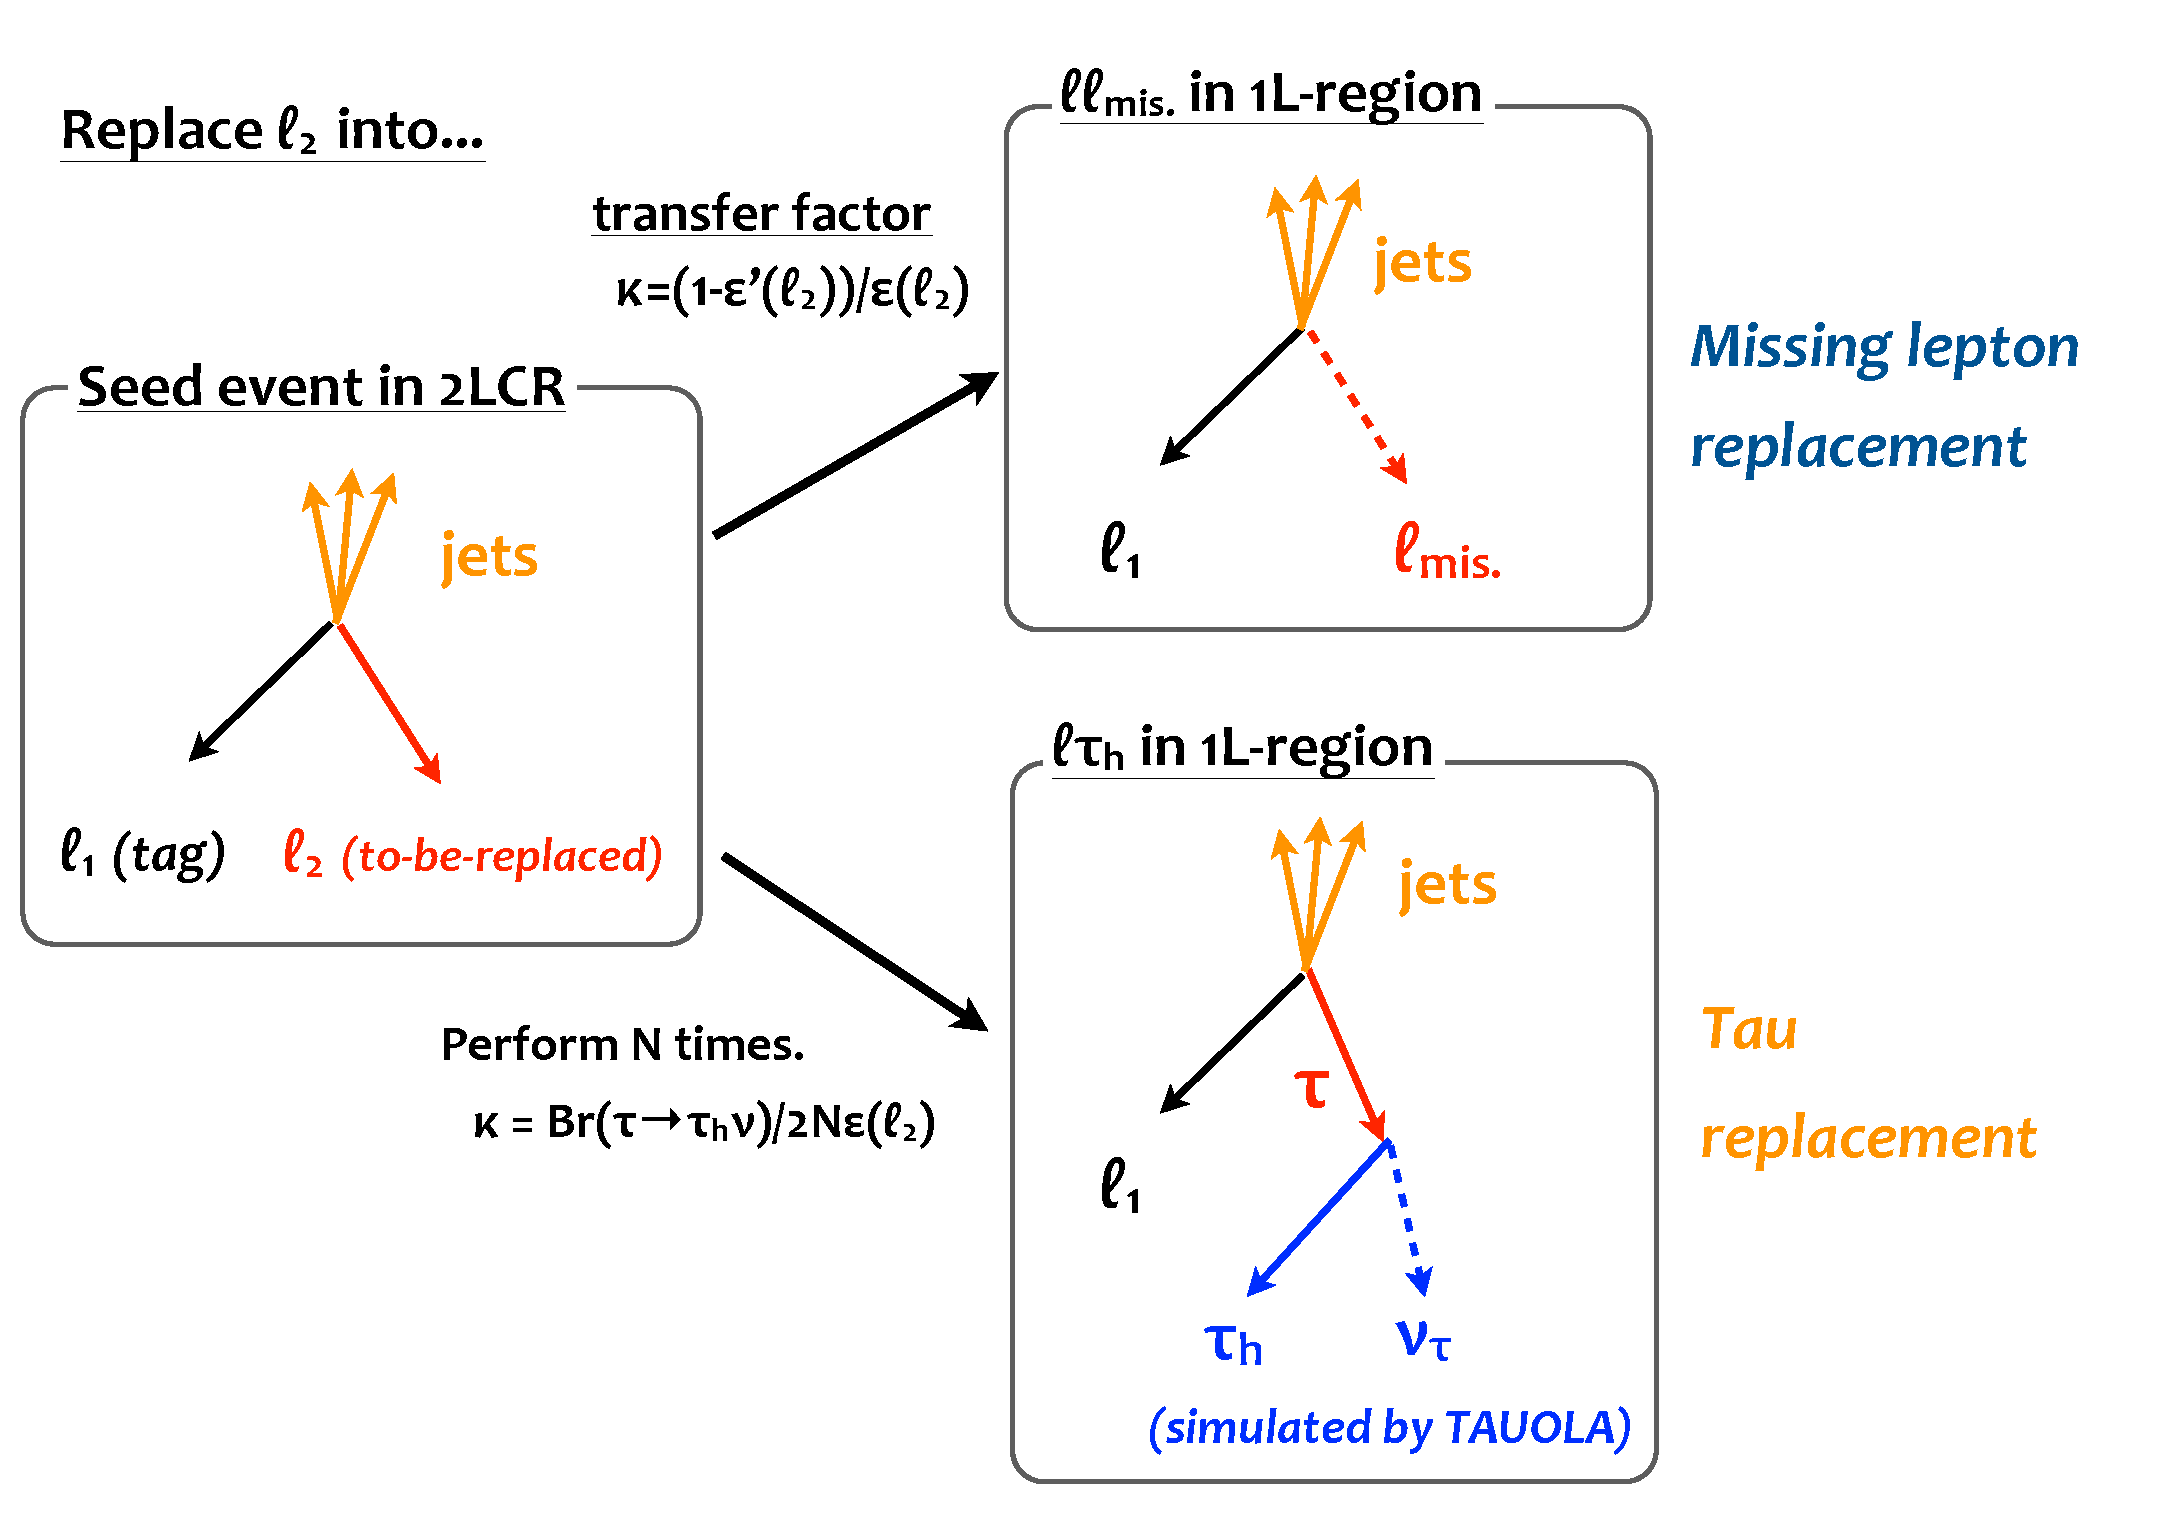
\includegraphics[width=160mm]{figures/BGestimation/ObjReplacement/method/schematic_replacement.eps}
\captionof{figure}{Schematic of the object replacement method.}
\label{fig::ObjReplace::schematic1}
\begin{center}
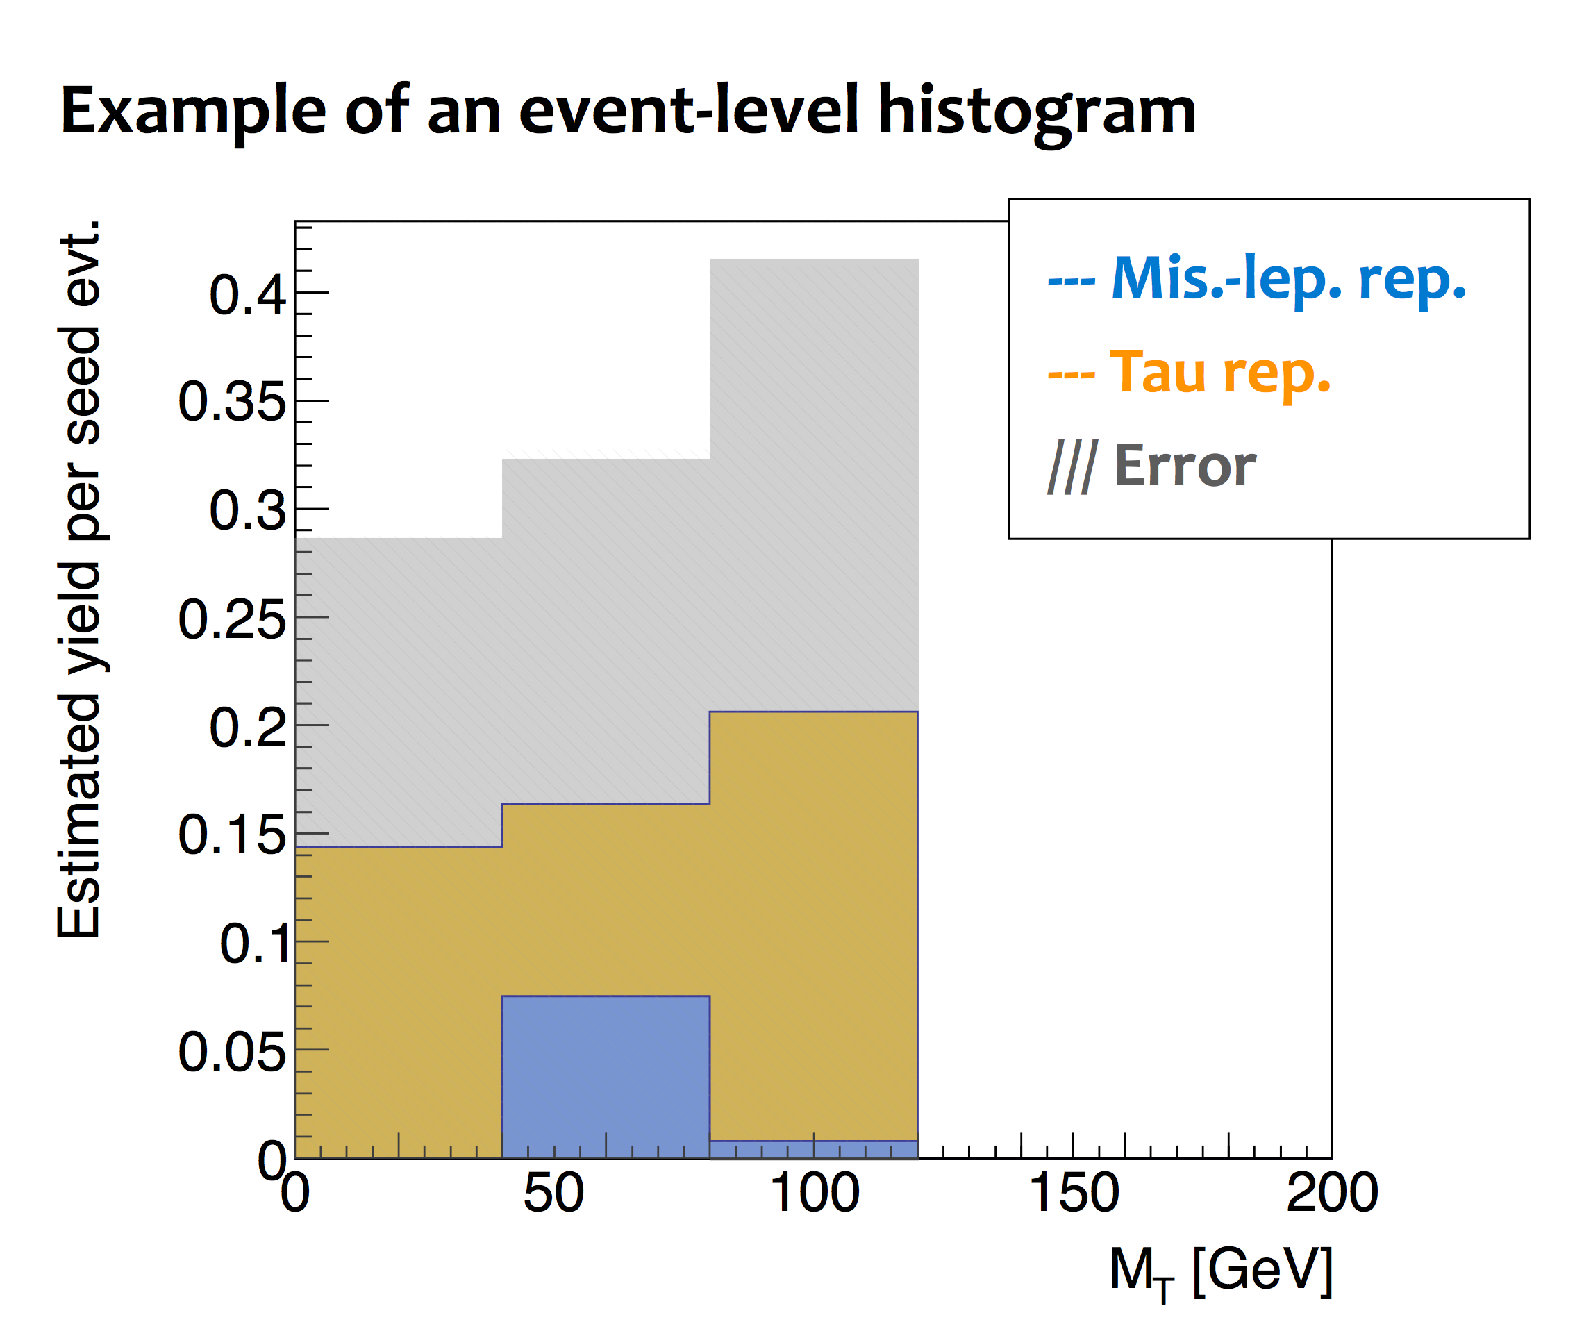
\includegraphics[width=80mm]{figures/BGestimation/ObjReplacement/method/evtLevel_histogram.eps}
\captionof{figure}{An example of event-level histogram. 100$\%$ uncertainty is assigned for each bin to account for the fact that all the entries are from the same seed. Final estimation is given by the sum of the event-level histograms over all seed events.}
\label{fig::ObjReplace::evtLevelHist}
\end{center}
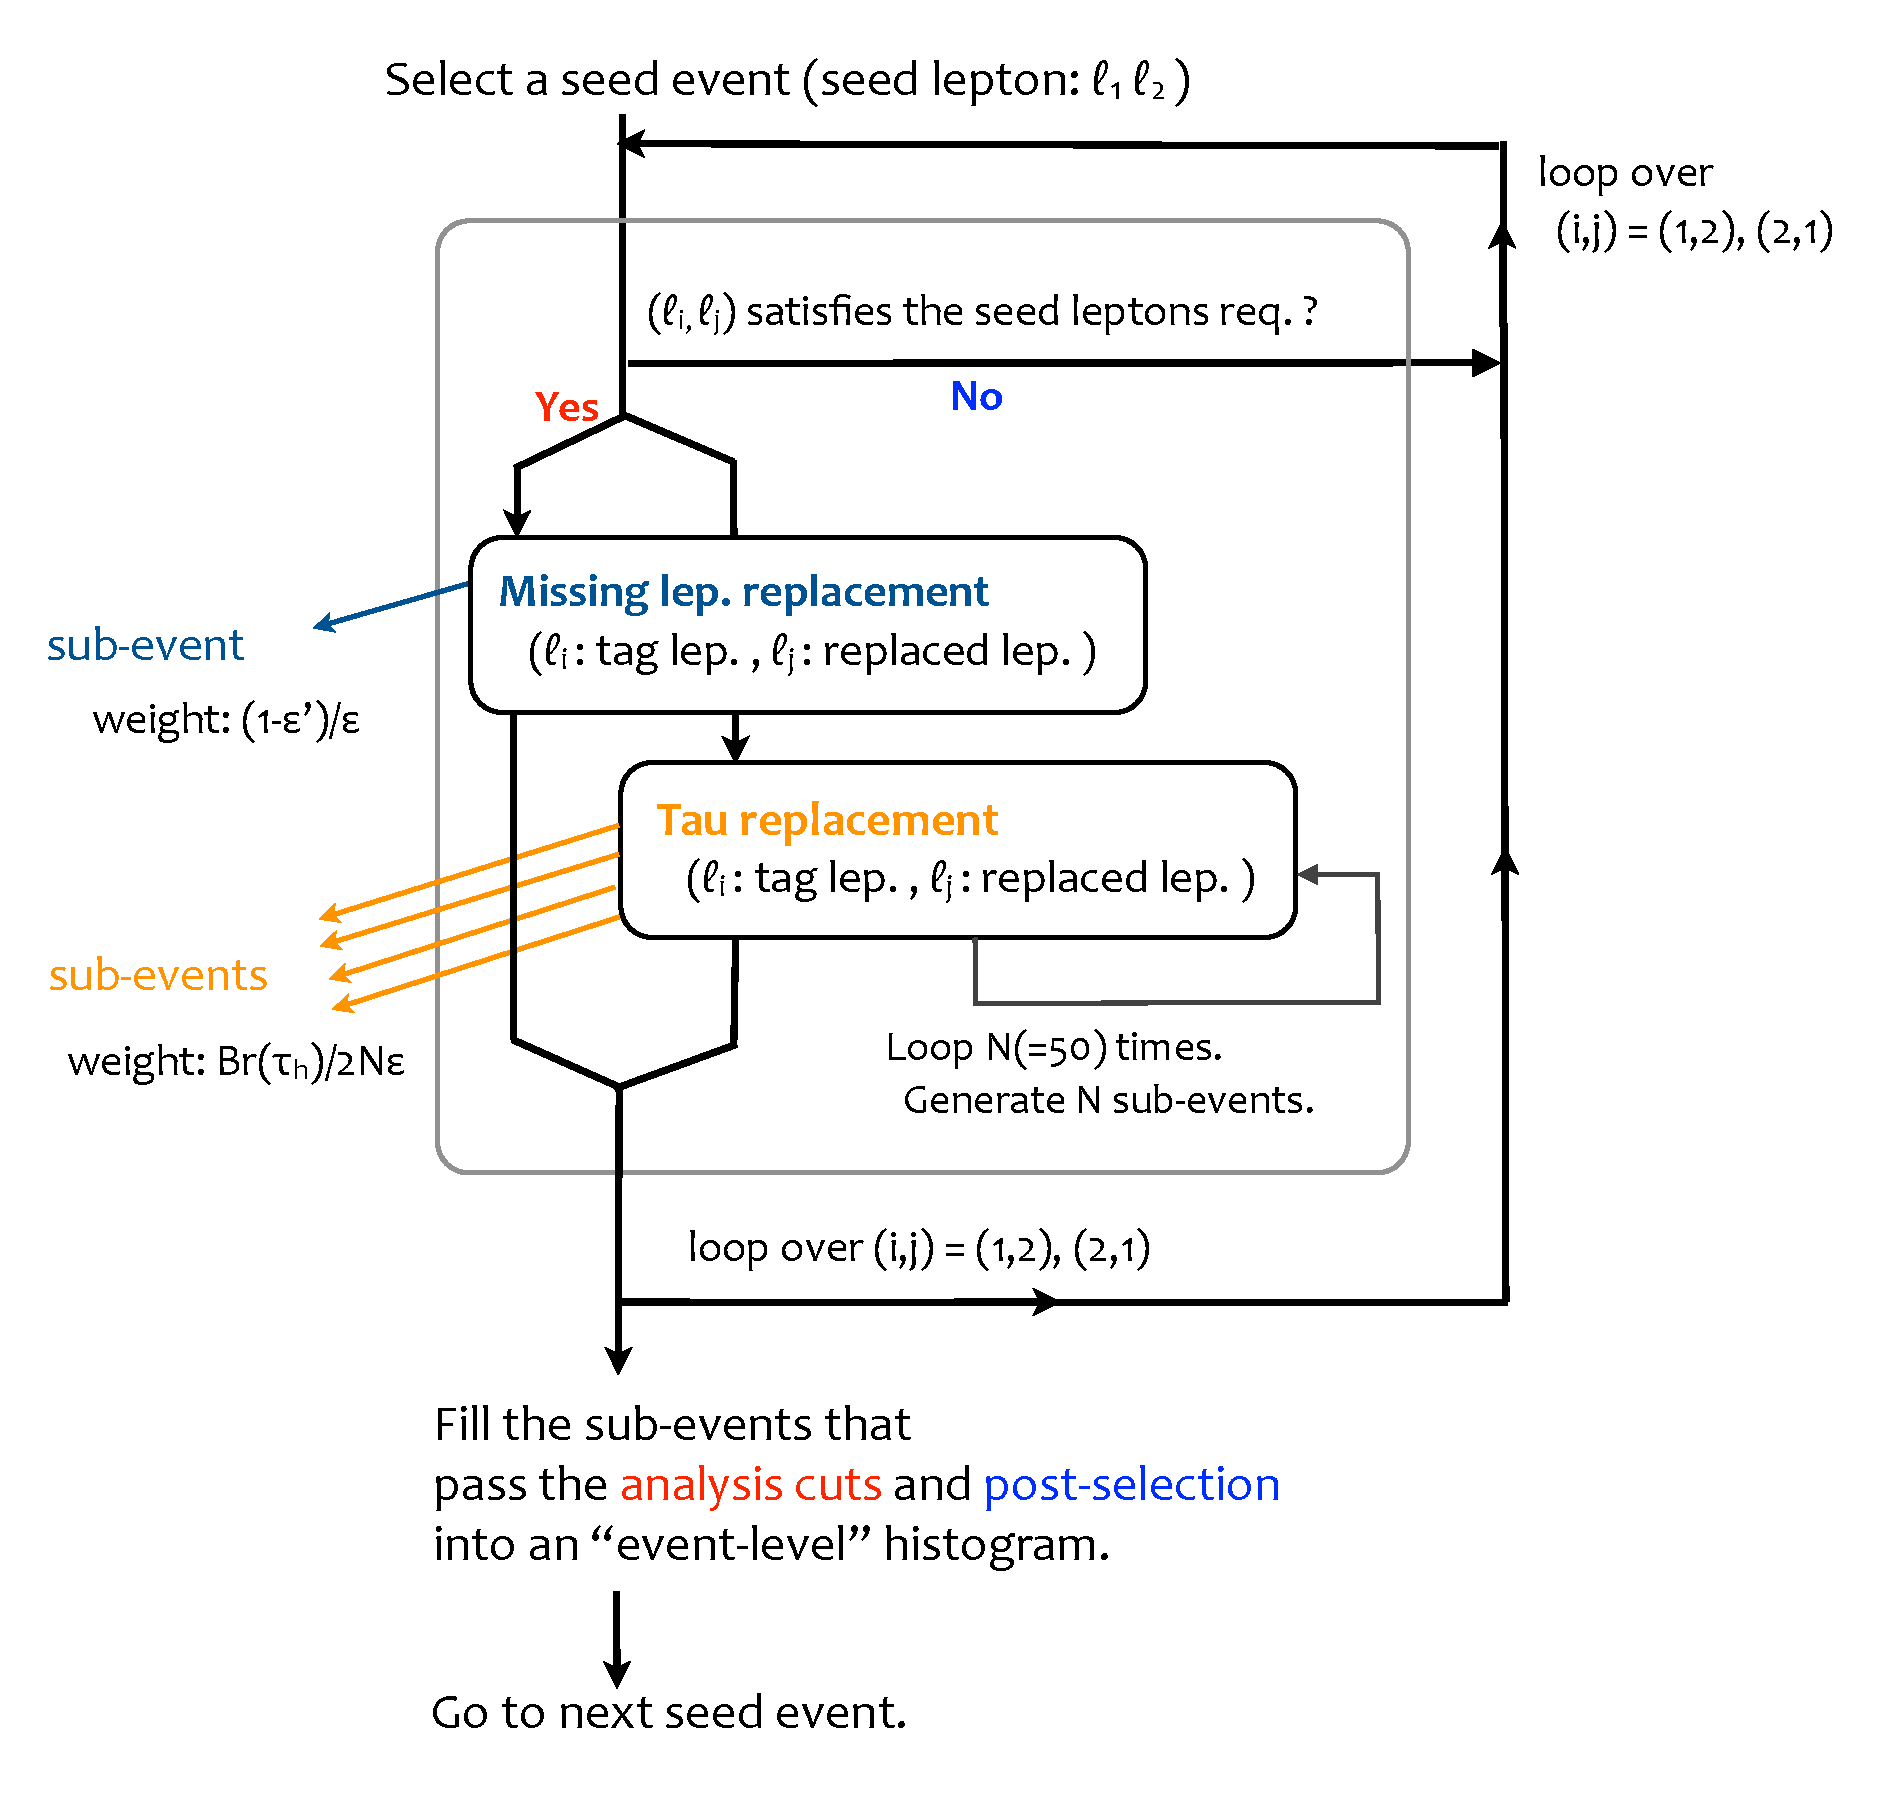
\includegraphics[width=160mm]{figures/BGestimation/ObjReplacement/method/flow_replacement.eps}
\captionof{figure}{Flow chart of actions per seed event.}
\label{fig::ObjReplace::schematic2}
%-------------------------------

More detail and caveats about each step are as following:  \\

\noindent \textbf{Seed event selection and trigger} \\
For seed event selection, looser kinematical selection is in general preferred to cover the full phase space to be estimated, within an acceptable level of contamination from irrelevant BGs (Z+jets, W+fakes etc.). 
In particular MET selection has to be loosened to at least around $E_{T}^{miss}>100\gev$ to fully account for the hard lepton signal regions where typically MET is required above $200\sim250\gev$. The single-lepton trigger is used to trigger such seed events, and the inversed efficiency (fig. \ref{fig::ObjReplace::method::SLTeff}) is applied event-by-event to accommodate the different triggers in use with respect to the analysis. In contrast, seed events are triggered by the MET trigger in estimating soft lepton signal regions (``2J'') as the tag lepton is not sufficiently hard to fire the single-lepton trigger. Thanks to the fact that the MET requirement in 2J is much higher ($E_{T}^{miss}>430\gev$), $E_{T}^{miss}>200\gev$ for seed selection is still affordable. To summarize, 2LCR is defined by the OR of two orthogonal regions (2LCRa and 2LCRb) as tab.\ref{tab::ObjReplace::method::2LCR}. \\

% ------------- 
\begin{table}[h]
  \begin{center}
    \caption{Definition of 2LCR. 2LCRa is aimed for estimating hard lepton regions (4Jlow-$x$, 4Jhigh-$x$, 6J) while 2LCRb is for soft lepton regions (2J).}
    \begin{tabular}{ | c | c | }
      \hline
      \multirow{4}{*}{2LCRa} 
      & $n_{\ell}(\mathrm{baseline})=2$, $n_{\ell}(\mathrm{signal})\ge1$ \\
      & $p_{T}(\ell_{1})>35\gev$, $|\eta(\ell)|<2.5$,  \\
      & At least one lepton fires the single-lepton trigger \\       
      & $\slashed{E}_{\mathrm{T}}$>100$\gev$, $n_J>=3$ \\
      \hline
      \multirow{4}{*}{2LCRb} 
      & $n_{\ell}(\mathrm{baseline})=2$, $n_{\ell}(\mathrm{signal})\ge1$ \\
      & $p_{T}(\ell_{1})<35\gev$, $|\eta(\ell)|<2.5$,  \\
      & MET trigger \\       
      & $\slashed{E}_{\mathrm{T}}$>200$\gev$, $n_J>=1$ \\
      \hline
    \end{tabular}  \label{tab::ObjReplace::method::2LCR}
  \end{center}
\end{table}


% -------------- method::2LCR
\begin{figure}[h]
  \centering
    \subfigure[]{\includegraphics[width=0.48\textwidth]{figures/BGestimation/ObjReplacement/method/met__2LCRa.eps}}
    \subfigure[]{\includegraphics[width=0.48\textwidth]{figures/BGestimation/ObjReplacement/method/lep2Pt__2LCRa.eps}}
    \caption{(a) MET and (b) second leading lepton Pt in 2LCRa. No QCD component (multi-jets, W+jets) is found beyond expectation. \label{fig::ObjReplace::method::2LCRa}}    
\end{figure}
%%%
\begin{figure}[h]
  \centering
    \subfigure[]{\includegraphics[width=0.31\textwidth]{figures/BGestimation/ObjReplacement/method/met__2LCRb.eps}}
    \subfigure[]{\includegraphics[width=0.31\textwidth]{figures/BGestimation/ObjReplacement/method/lep1Pt__2LCRb.eps}}
    \subfigure[]{\includegraphics[width=0.31\textwidth]{figures/BGestimation/ObjReplacement/method/lep2Pt__2LCRb.eps}}
    \caption{(a) MET, (b) leading lepton Pt and (c) second leading lepton Pt in 2LCRb.  \label{fig::ObjReplace::method::2LCRb}}    
\end{figure}
%-------------------------------

% -------------- method::SLTeff
\begin{figure}[h]
  \centering
    \subfigure[]{\includegraphics[width=0.48\textwidth]{figures/BGestimation/ObjReplacement/method/SingleElectronTriggerEff.eps}}
    \subfigure[]{\includegraphics[width=0.441\textwidth]{figures/BGestimation/ObjReplacement/method/SingleMuonTriggerEff.eps}}
    \caption{Trigger efficiency of (a) single electron and (b) single muon trigger, defined by the fraction of offline leptons matched with online objects. Efficiencies are parameterized as function of pt and eta of the lepton. All computed using ttbar MC.  \label{fig::ObjReplace::method::SLTeff}}    
\end{figure}
%----------------------------------

\noindent \textbf{Tag lepton requirement} \\
As the tag lepton is equivalent to the lepton used in the analysis in 1L regions, it has to satisfy the signal lepton requirement (as well as $p_{T}>30\gev$ and the trigger matching in case of estimating hard lepton regions). \\
%-

\noindent \textbf{Treatment of virtual missing lepton} \\
As electrons are reconstructed as jets as well in most cases, electrons failing reconstruction or ID will be recognized as jets in this analysis. Therefore in the missing lepton replacement, if there is at least one reconstructed jet overlapped with the electron to be replaced by $\Delta R<0.4$, the electron will be replaced into the closest jet, otherwise into a missing particle inheriting the momentum of original electron.
Missing muons will be usually not identified as any objects. However they are still counted in the MET track soft term in some occasion. Since the criteria are complicated and also keeps evolving all the time, we ignore it for the moment and simply treat all missing lepton as missing particles. The impact might not be negligible for missing muon estimation, but given the very high efficiency of muon reconstruction and ID, the impact on final estimation should be limited.  \\

\noindent \textbf{Simulation of tau decays} \\
Tau decays are simulated by TAUOLA \cite{rep::TAUOLA} assuming the taus are unpolarized. This assumption is incorrect given the parent W-bosons are left-handed, but the impact on the final result is studied (see below chapter) and found to be marginal. Branching for leptonic decay is set to zero to reduce the number of loops. \\

Given that the analysis is tau-agonistic, hadronic taus within $p_{\mathrm{T}}$-$\eta$ acceptance are reconstructed and recognized as full-calibrated anti-Kt4 jets once they pass the JVT cut. On the other hand, the output of TAUOLA is merely a 4-vector of truth level hadronic tau. Therefore following treatments are applied for the truth-level hadronic taus to emulate observables.\\

\begin{enumerate}
\item Apply the scale of anti-Kt4 jets for truth hadronic taus. \\
Due to the fact that the anti-Kt4 jet have larger cone and contain more underlying tracks inside, the measured energy will be systematically higher than the truth when a hadronic tau is measured as an anti-Kt4 jet. To emulate the effect, a scale is applied for truth hadronic taus output from TAUOLA. \\

\item Smear the $p_{\mathrm{T}}$ of hadronic tau. \\
To account for the resolution of measurement, a simple Gaussian smearing is applied for $p_{\mathrm{T}}$ of hadronic taus after correcting the scale. \\

These scale and resolution are derived from $t\bar{t}$ MC by comparing the $p_{\mathrm{T}}$ of truth hadronic taus and that of $\Delta R$-matched reconstructed jet by $\Delta R<0.2$, as a function of $p_{\mathrm{T}}$ and $\eta$ of truth hadronic taus (fig.\ref{fig::ObjReplace::tau_scale}, \ref{fig::ObjReplace::tau_resol}).

\item Emulate signal jet identification / b-tagging  \\
Hadronic taus with $p_{\mathrm{T}}>30\gev$, $|\eta|<2.8$ are selected as the signal jet candidates.
%, based on the scaled and smeared $p_{\mathrm{T}}$. 
Signal jets are then randomly identified from them, based on the efficiency of JVT cut. A random b-tagging is further performed on the signal jets, by assigning a random b-tagging score (MV2c10) following according to the profile. The JVT cut efficiency and profile of b-tagging score are obtained by $t\bar{t}$ MC using jets matched with truth hadronic taus by $\Delta R<0.2$. JVT cut efficiency is parameterized as a function of $p_{\mathrm{T}}$ and $\eta$ of signal jet candidates (fig.\ref{fig::ObjReplace::effJVT}), while the b-tagging score profile is separately derived by tau decay modes (fig.\ref{fig::ObjReplace::tau_bTagScore}).
\end{enumerate}


\noindent \textbf{Transfer factor} \\
A weight $\kappa$ is assigned on each sub-event to account for the different probability of occurance between the seed event and the replaced sub-event. For instance in the missing lepton replacement, this corresponds to the efficiency ($\epsilon_{\mathrm{baseline}}(\ell_{\mathrm{rep.}})$) and inefficiency ($1-\epsilon_{\mathrm{Reco.+ID}}(\ell_{\mathrm{rep.}})$) of offline lepton selection for the replaced lepton. The ratio 
$$\kappa=\frac{1-\epsilon_{\mathrm{Reco.+ID}}(\ell_{\mathrm{rep.}})}{\epsilon_{\mathrm{baseline}}(\ell_{\mathrm{rep.}})}$$
has to be applied to get the correct normalization of estimation. \\

As for the tau replacement, the transfer factor is 
$$\kappa=\frac{\mathrm{Br}(\tau\rightarrow\tau_{\mathrm{h}}\nu)}{2N\epsilon_{\mathrm{baseline}}(\ell_{\mathrm{rep.}})}$$,
where N is number of iteration per replacement which is currently set to 50 ($N$ merely defines the level of ``smoothing'' thus has no essential impact on the final result). The factor 2 reflects the fact that two channels ($e\ell$ and $\mu\ell$) are available as seeds. \\
$1/\kappa$ roughly indicates the ratio of statistics between CR and SR. Giving that the sub-events of missing lepton replacement and tau replacement originate from the common seed events, and that generally $\ell\tau_{\mathrm{h}}$ populates much more than $\ell\ell_{\mathrm{mis.}}$, the effective CR statistics is no more than 3 times as SR statistics. This factor of 3 gain in statistics is in fact not very sufficient as it immediately leads to $30\% \sim 50\%$ statistical error by itself in typical signal regions where only a few events are expected. Therefore CR statistic is always the biggest source of uncertainty in this method. \\


\noindent \textbf{Lepton efficiency} \\
Lepton efficiency used in trasfer factor calculation is obtained by $t\bar{t}$ MC as a function of $p_{\mathrm{T}}$ and $\eta$ of truth leptons (fig.\ref{fig::ObjReplace::lep_efficiency}). The efficiency is defined as the fraction of truth leptons that are $\Delta R$-matched with reconstructed lepton passing ID or signal lepton requirement by $\Delta R<0.2$. \\


\noindent \textbf{Event-level histogram and statistical treatment} \\
Multiple sub-events are generated by both missing lepton replacement and tau replacement from a single seed event, and filled into the same event-level histogram. To account for this full correlation, $100\%$ error is assigned to each bin of the event-level histogram. 
The sum of event-level histograms over all seed events will be the desired distribution. Although the summation is not trivial since the bins of event-level histograms are not statistically independent each other, the effect of bin-to-bin correlation is supposed to be negligible considering that signal regions are single-binned or coarsely binned (much coarser than typical width of event-level histogram) in this analysis.

%
% ---------- method::plot
%%%%%%%% Method::tauRF
\clearpage
\begin{figure}[htbp]
  \begin{center}
      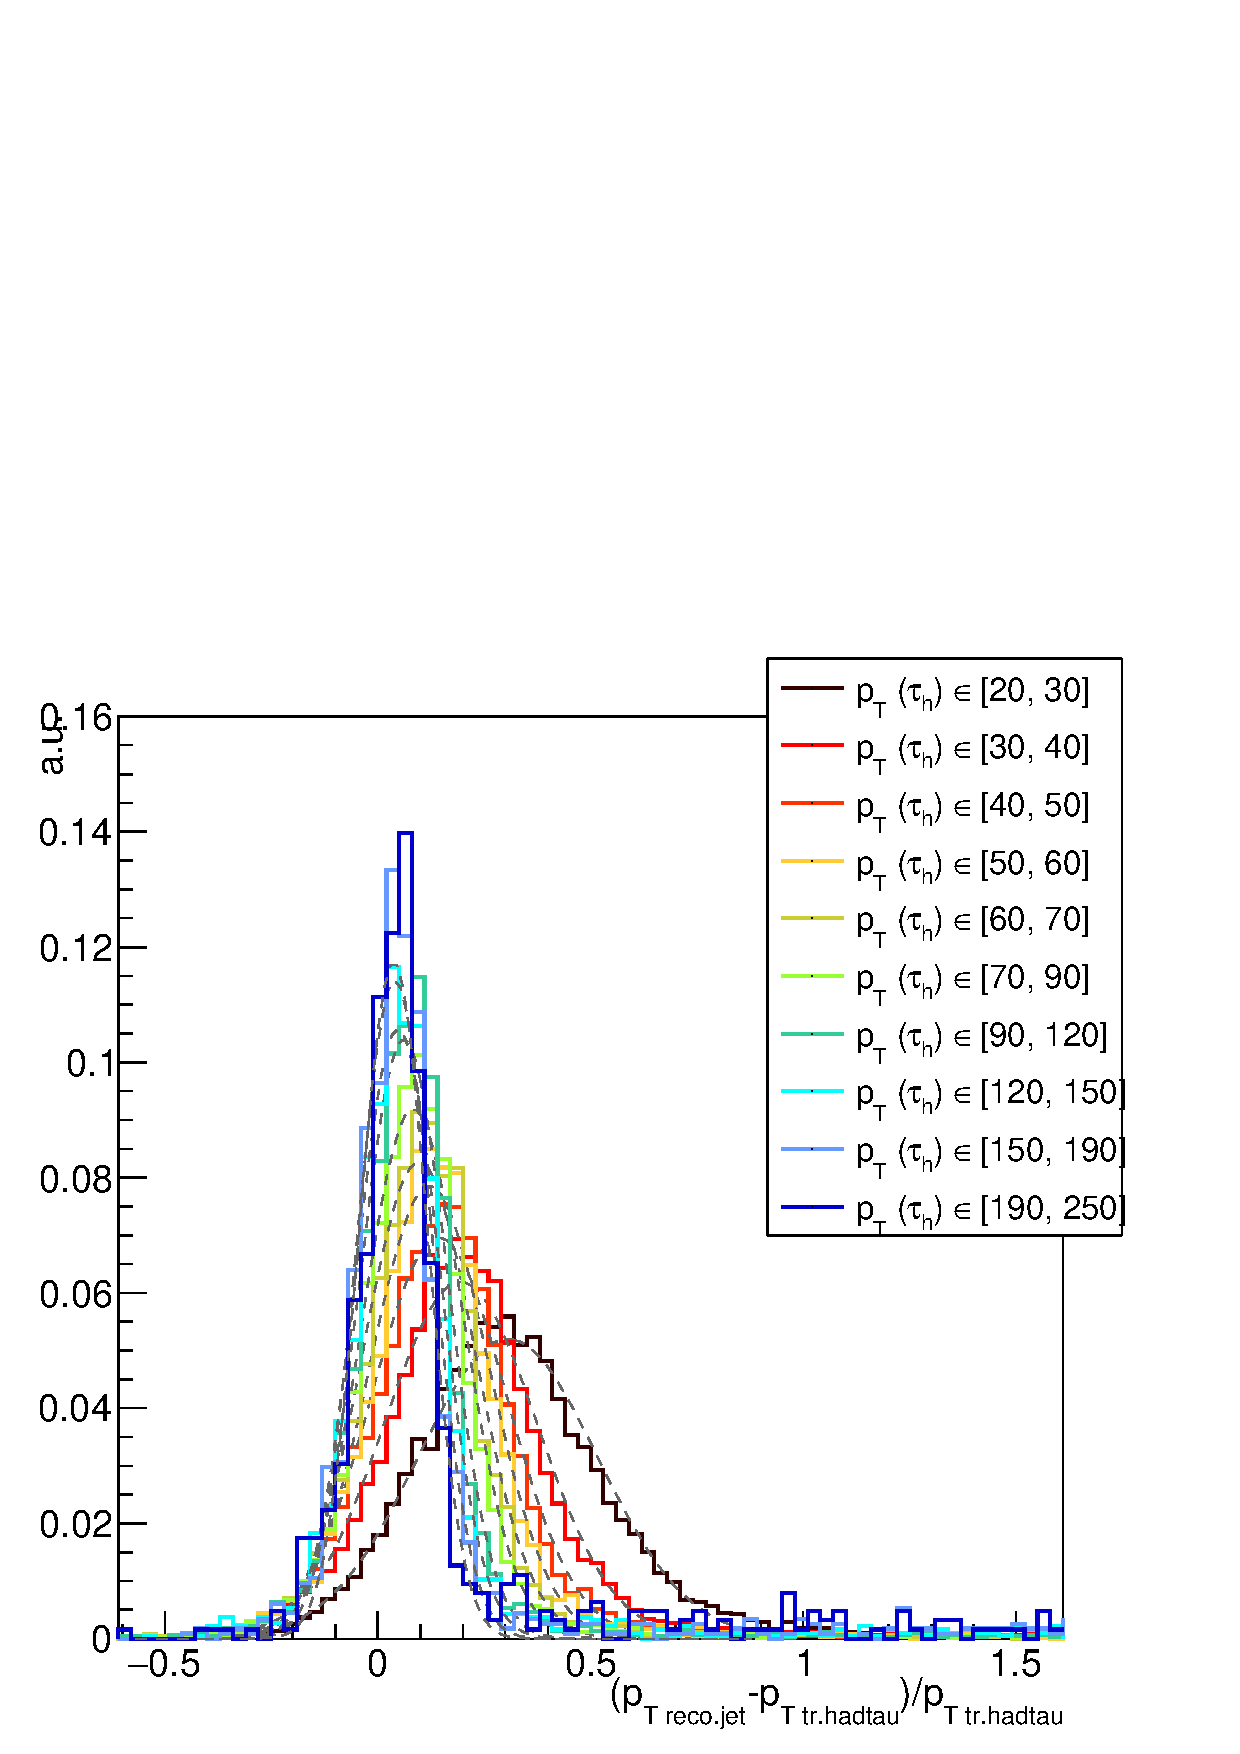
\includegraphics[width=100mm]{figures/BGestimation/ObjReplacement/method/tauRF/ptResidual.pdf} 
      \caption{}
      \label{fig::ObjReaplce::tau_ptResidual}
    %
    \begin{minipage}[t]{.45\textwidth}
      \centering        
      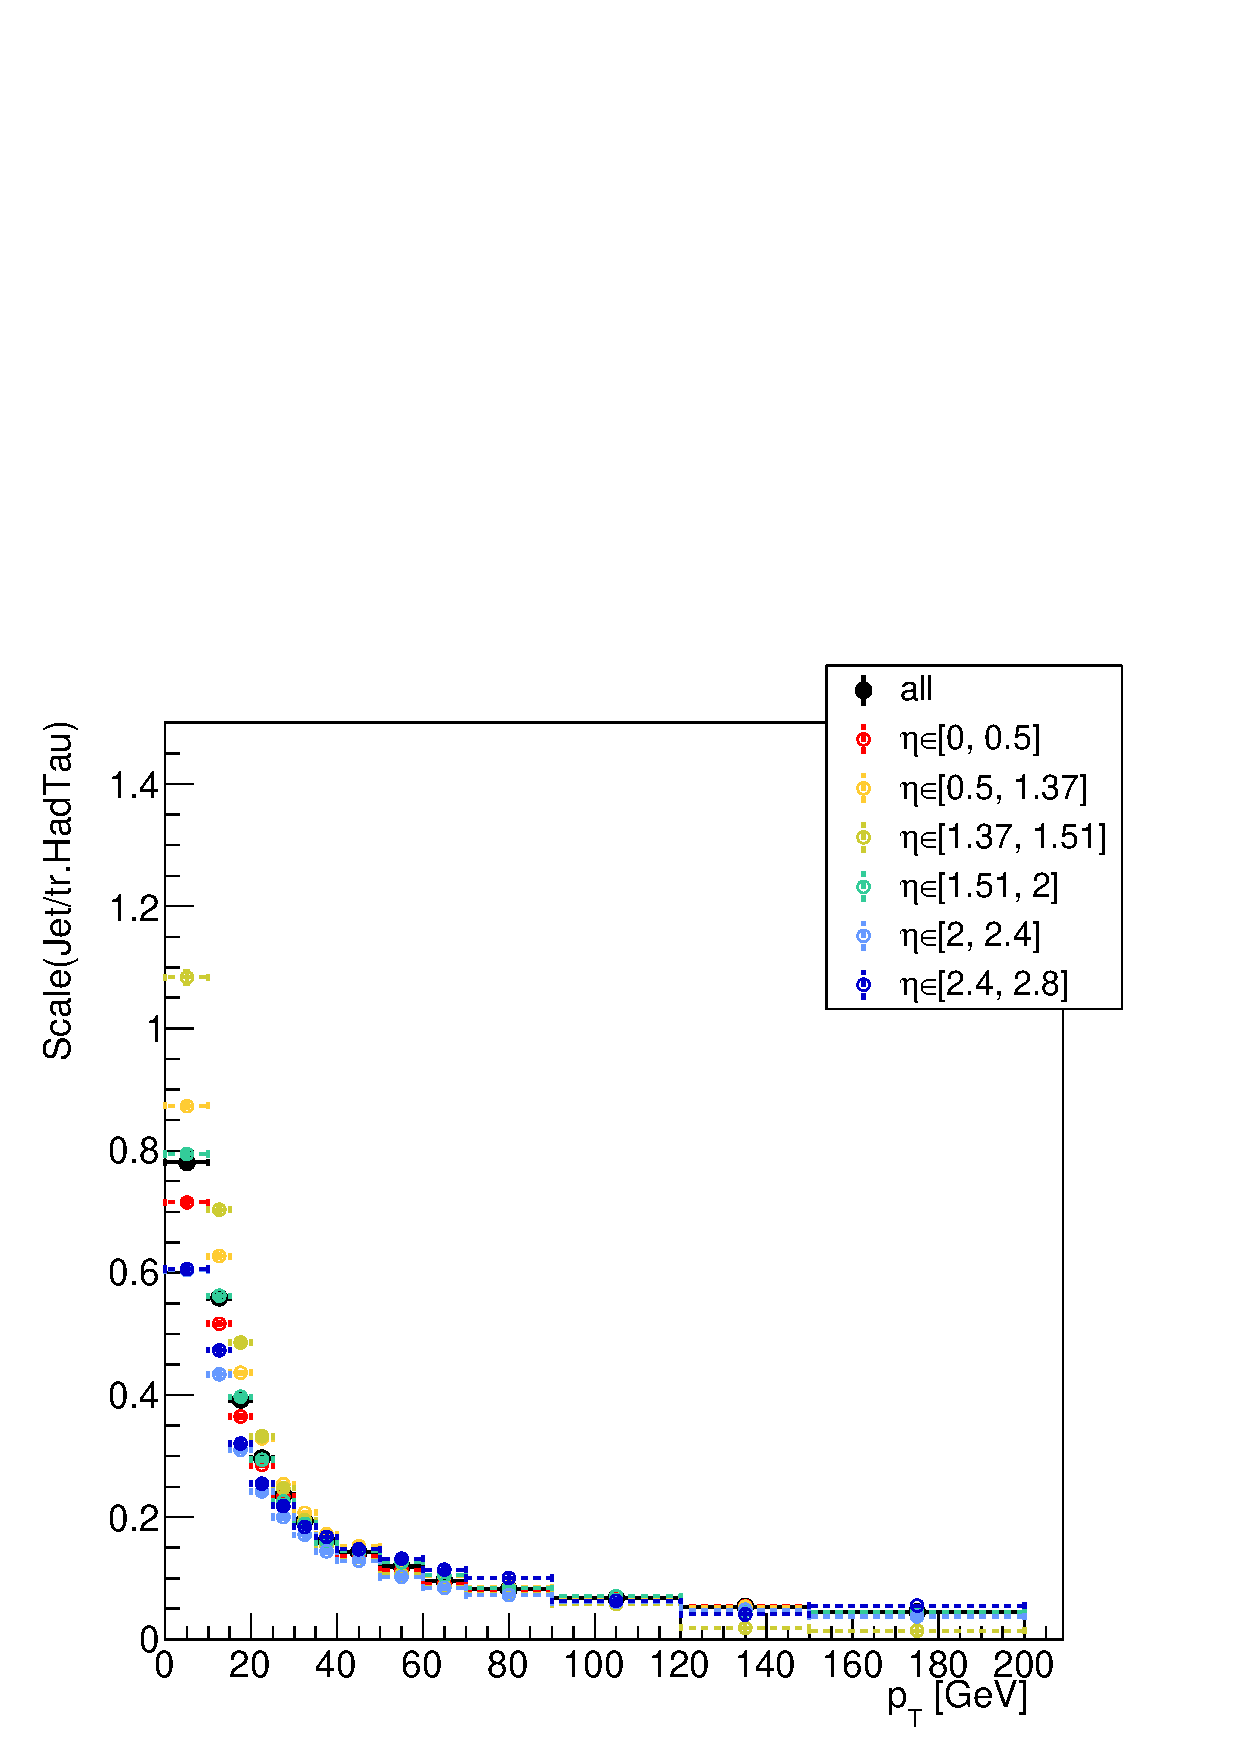
\includegraphics[width=85mm]{figures/BGestimation/ObjReplacement/method/tauRF/tauJet_scale.pdf} 
      \caption{Scale of anti-Kt4 jets for truth hadronic taus, defined as the mean of reco. $p_T(\tau_{h})$/truth $p_T(\tau_{h})-1$ distribution. Truth $p_T(\tau_{h})$ is defined as the transverse component of $|\bm{p}(\tau)-\bm{p}(\nu_{tau})|$ while the reconstructed one is defined as the $p_T$ of an anti-Kt4 jet $\Delta R$-matched to it.}
      \label{fig::ObjReaplce::tau_scale}
    \end{minipage}
    \hfill
    \begin{minipage}[t]{.45\textwidth}
      \centering
      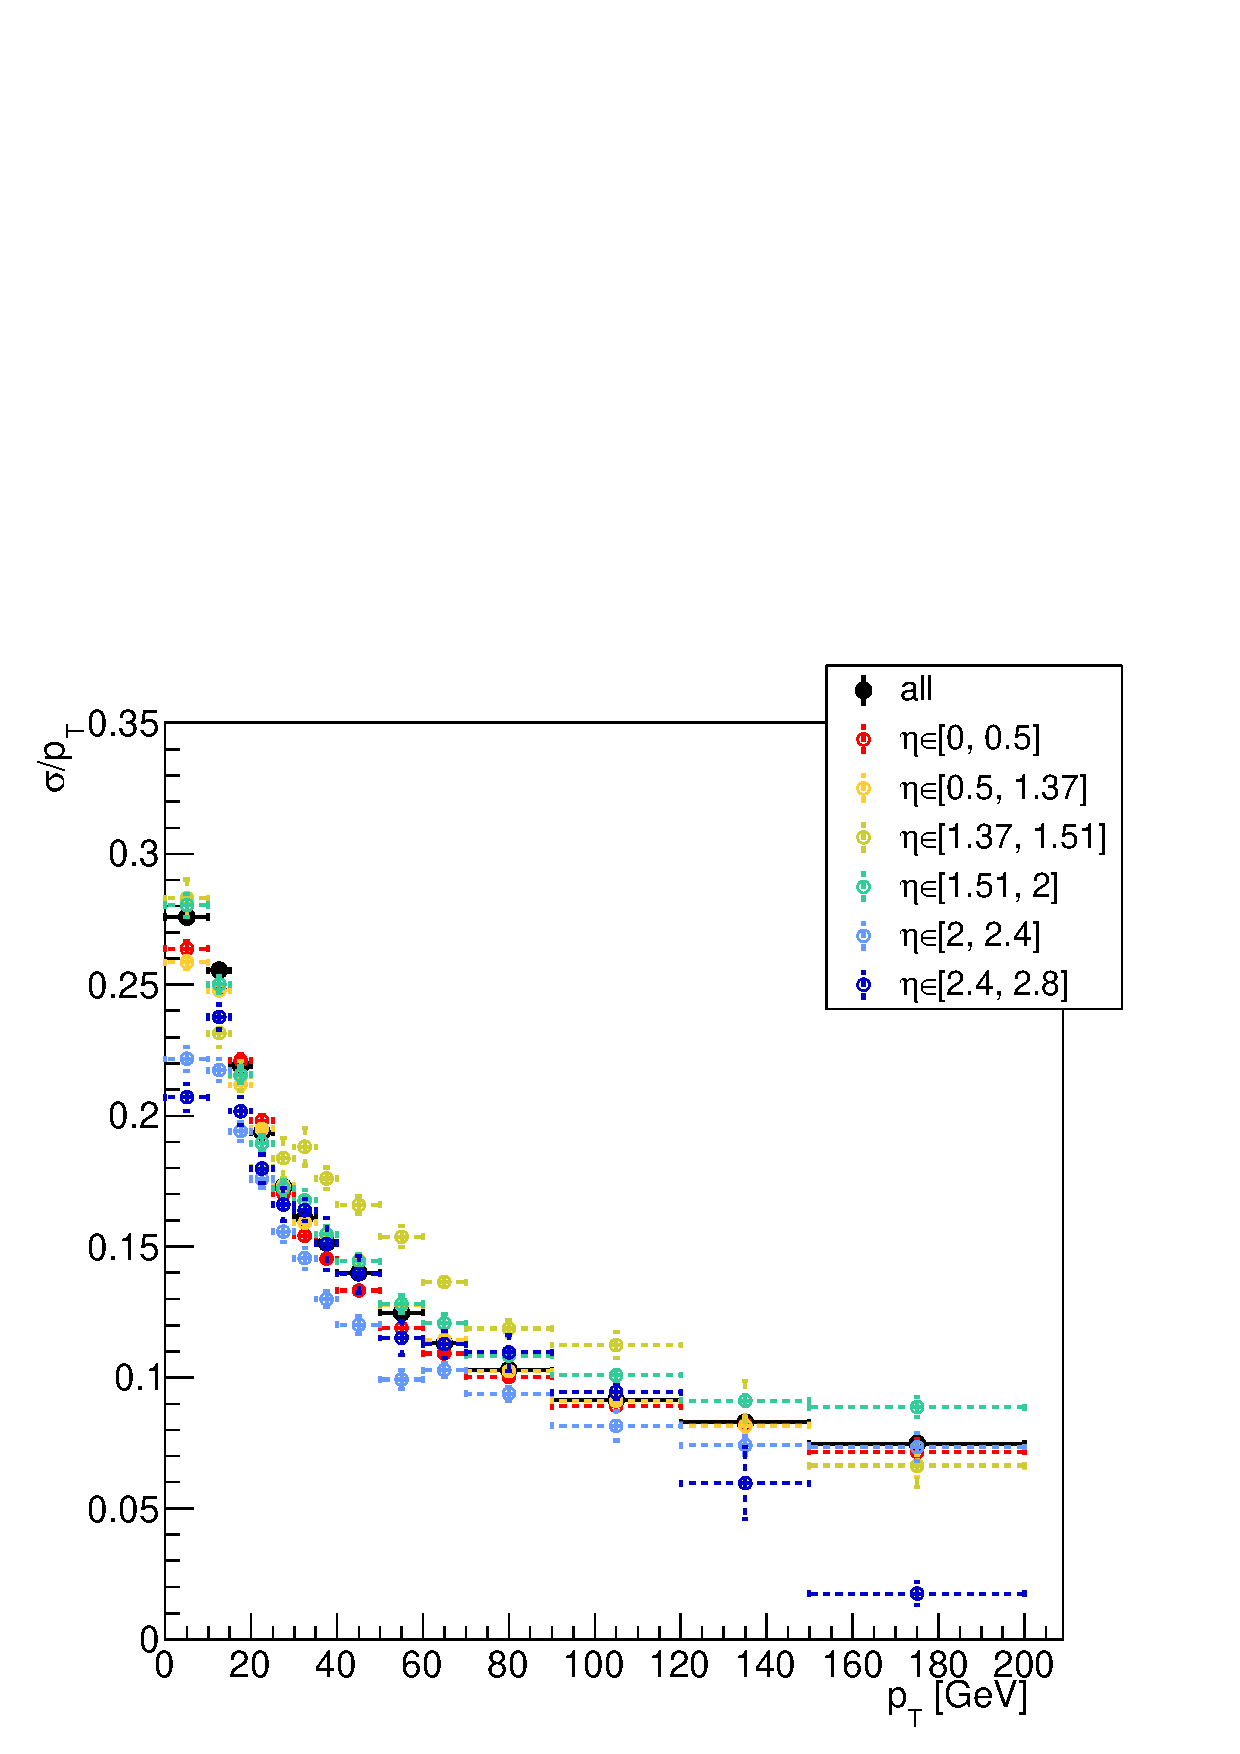
\includegraphics[width=85mm]{figures/BGestimation/ObjReplacement/method/tauRF/tauJet_resol.pdf}
      \caption{Resolution of hadronic tau, defined as the gaussian-fitted RMS of reco. $p_T(\tau_{h})$/truth $p_T(\tau_{h})-1$ distribution. Reco. $p_T(\tau_{h})$ is defined as the $p_T$ of $\Delta R$-matched anti-Kt4 jet.}
      \label{fig::ObjReaplce::tau_resol}
    \end{minipage}
    %              
  \end{center}  
\end{figure}
\clearpage
\begin{figure}[htbp]
  \begin{center}
    \begin{minipage}[t]{.45\textwidth}
      \centering
      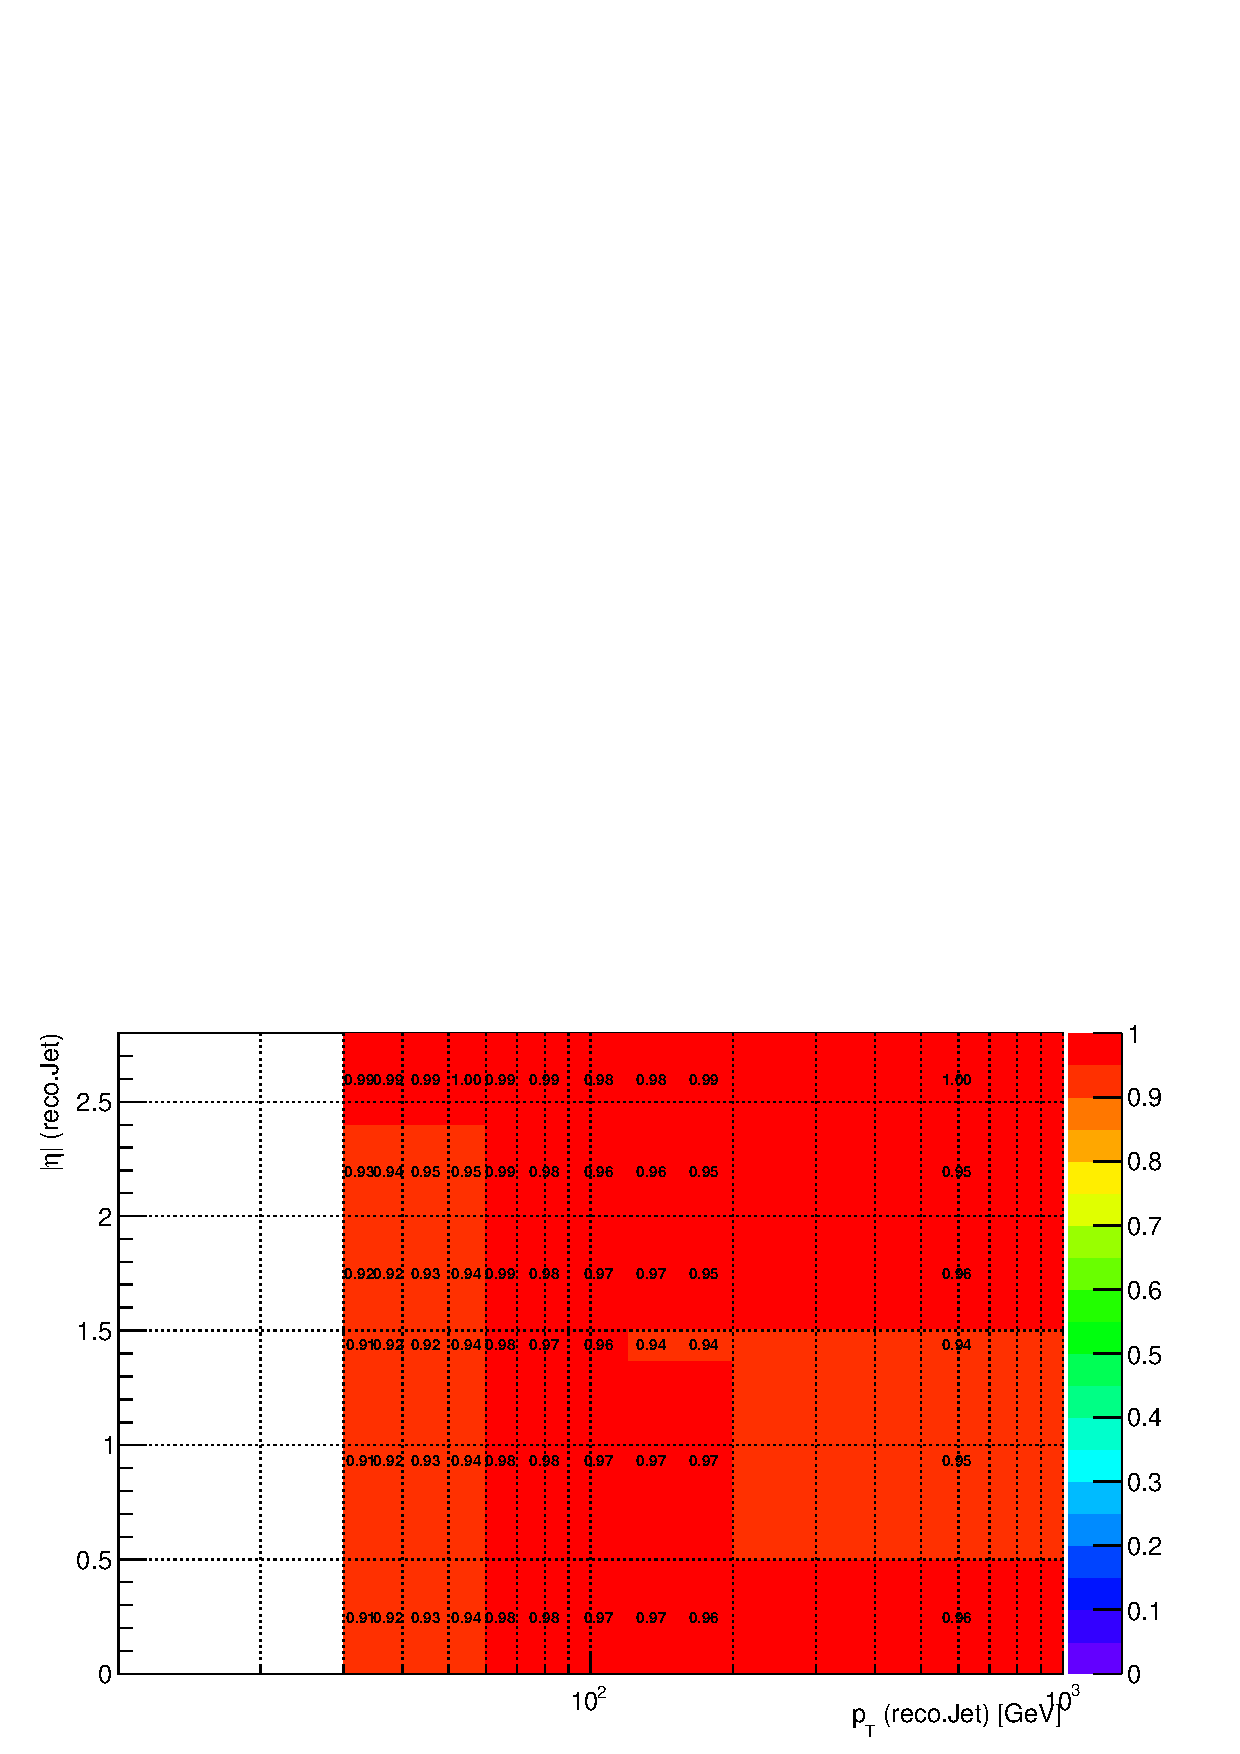
\includegraphics[width=85mm]{figures/BGestimation/ObjReplacement/method/tauRF/heff_vs_recoJetPt_recoJetEta.pdf}
      \caption{Fraction of signal jet candidates that pass the signal jet requirement, parametrized as function of $p_{\mathrm{T}}$ and $\eta$ of reconstructed jets.}
      \label{fig::ObjReaplce::effJVT}
    \end{minipage}
    \hfill
    \begin{minipage}[t]{.45\textwidth}
      \centering
      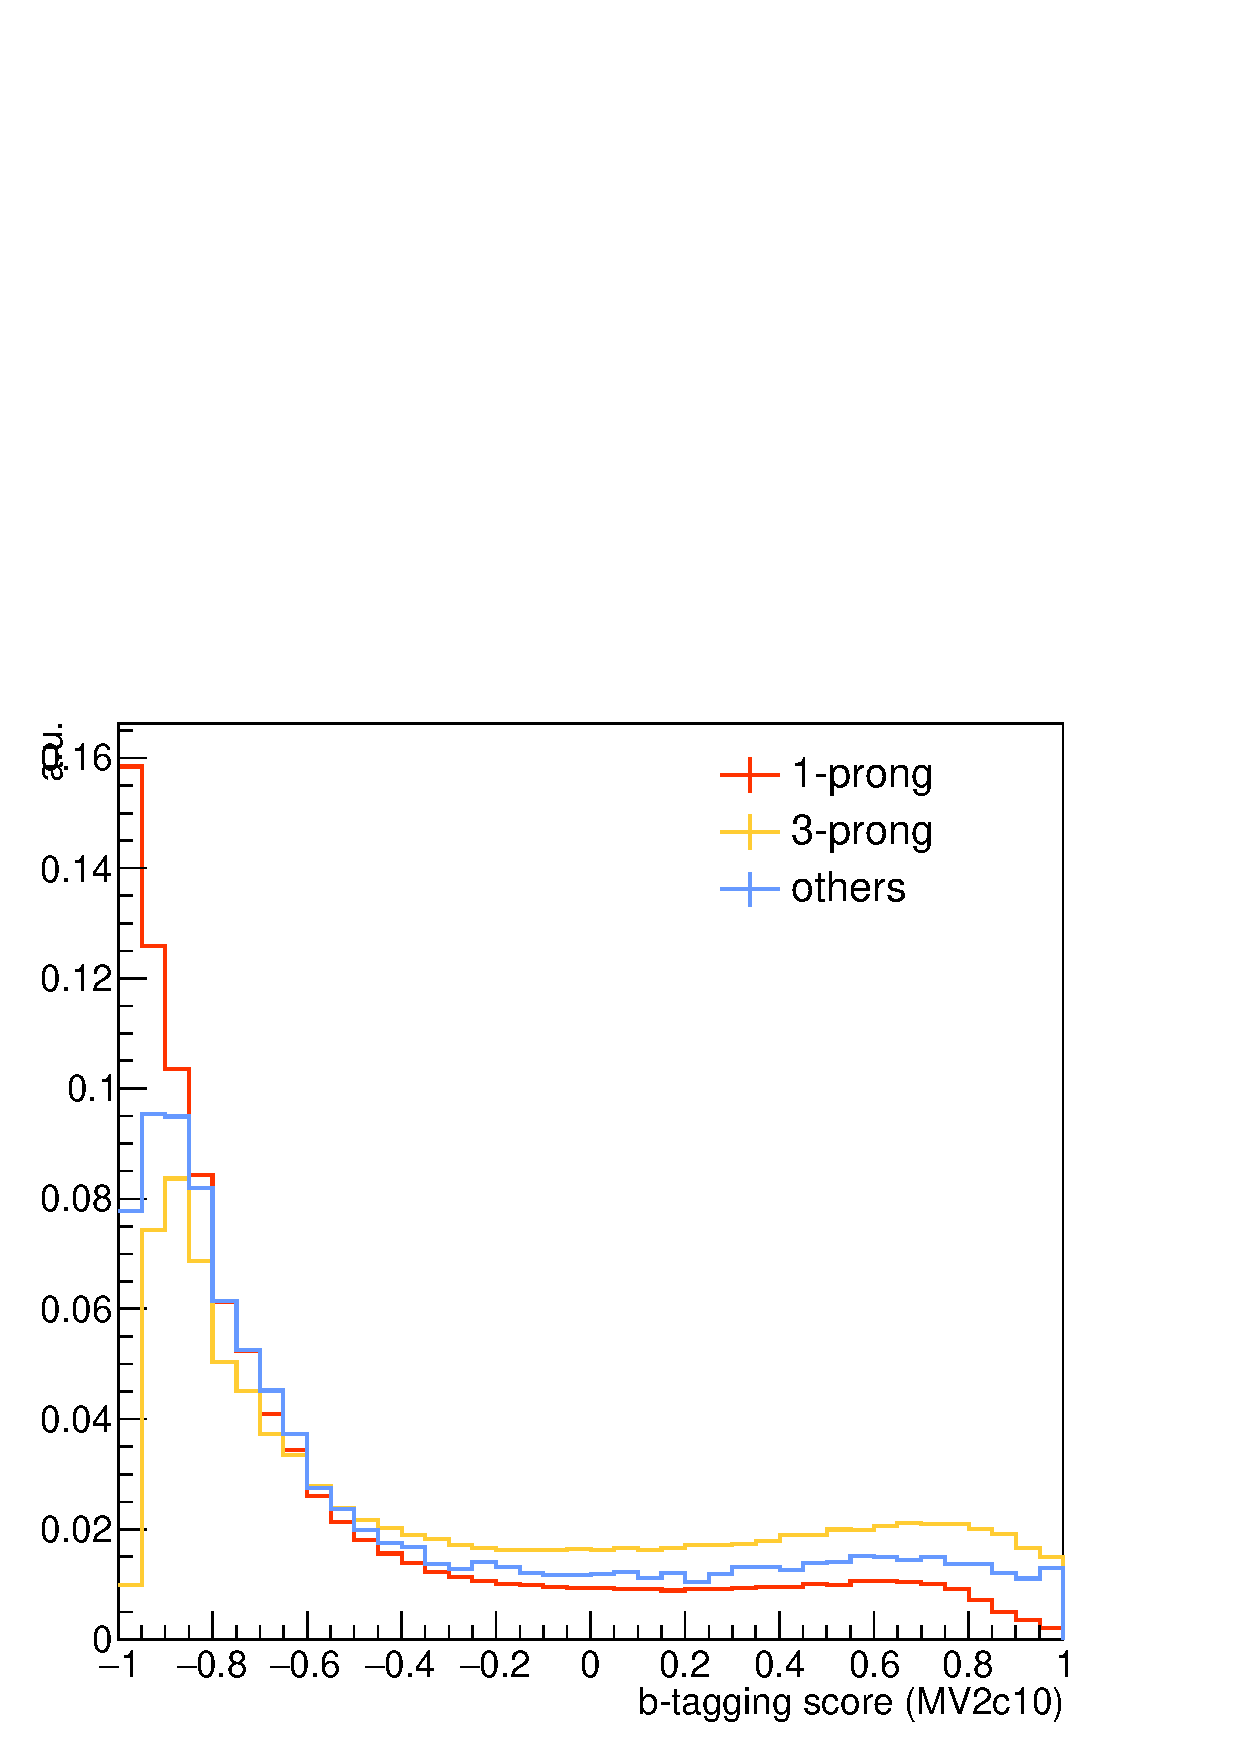
\includegraphics[width=75mm]{figures/BGestimation/ObjReplacement/method/tauRF/hadTau_bTagScore.pdf}
      \caption{Profile of b-tagging score (MV2c10) for tau jets, calculated from ttbar MC.}
      \label{fig::ObjReaplce::tau_bTagScore}
    \end{minipage}
    %
  \end{center}
\end{figure}
%%%%% Method::effMap 
%\clearpage
\begin{figure}[htbp]
  \begin{center}
    %
    \begin{minipage}[t]{.45\textwidth}
      \centering
      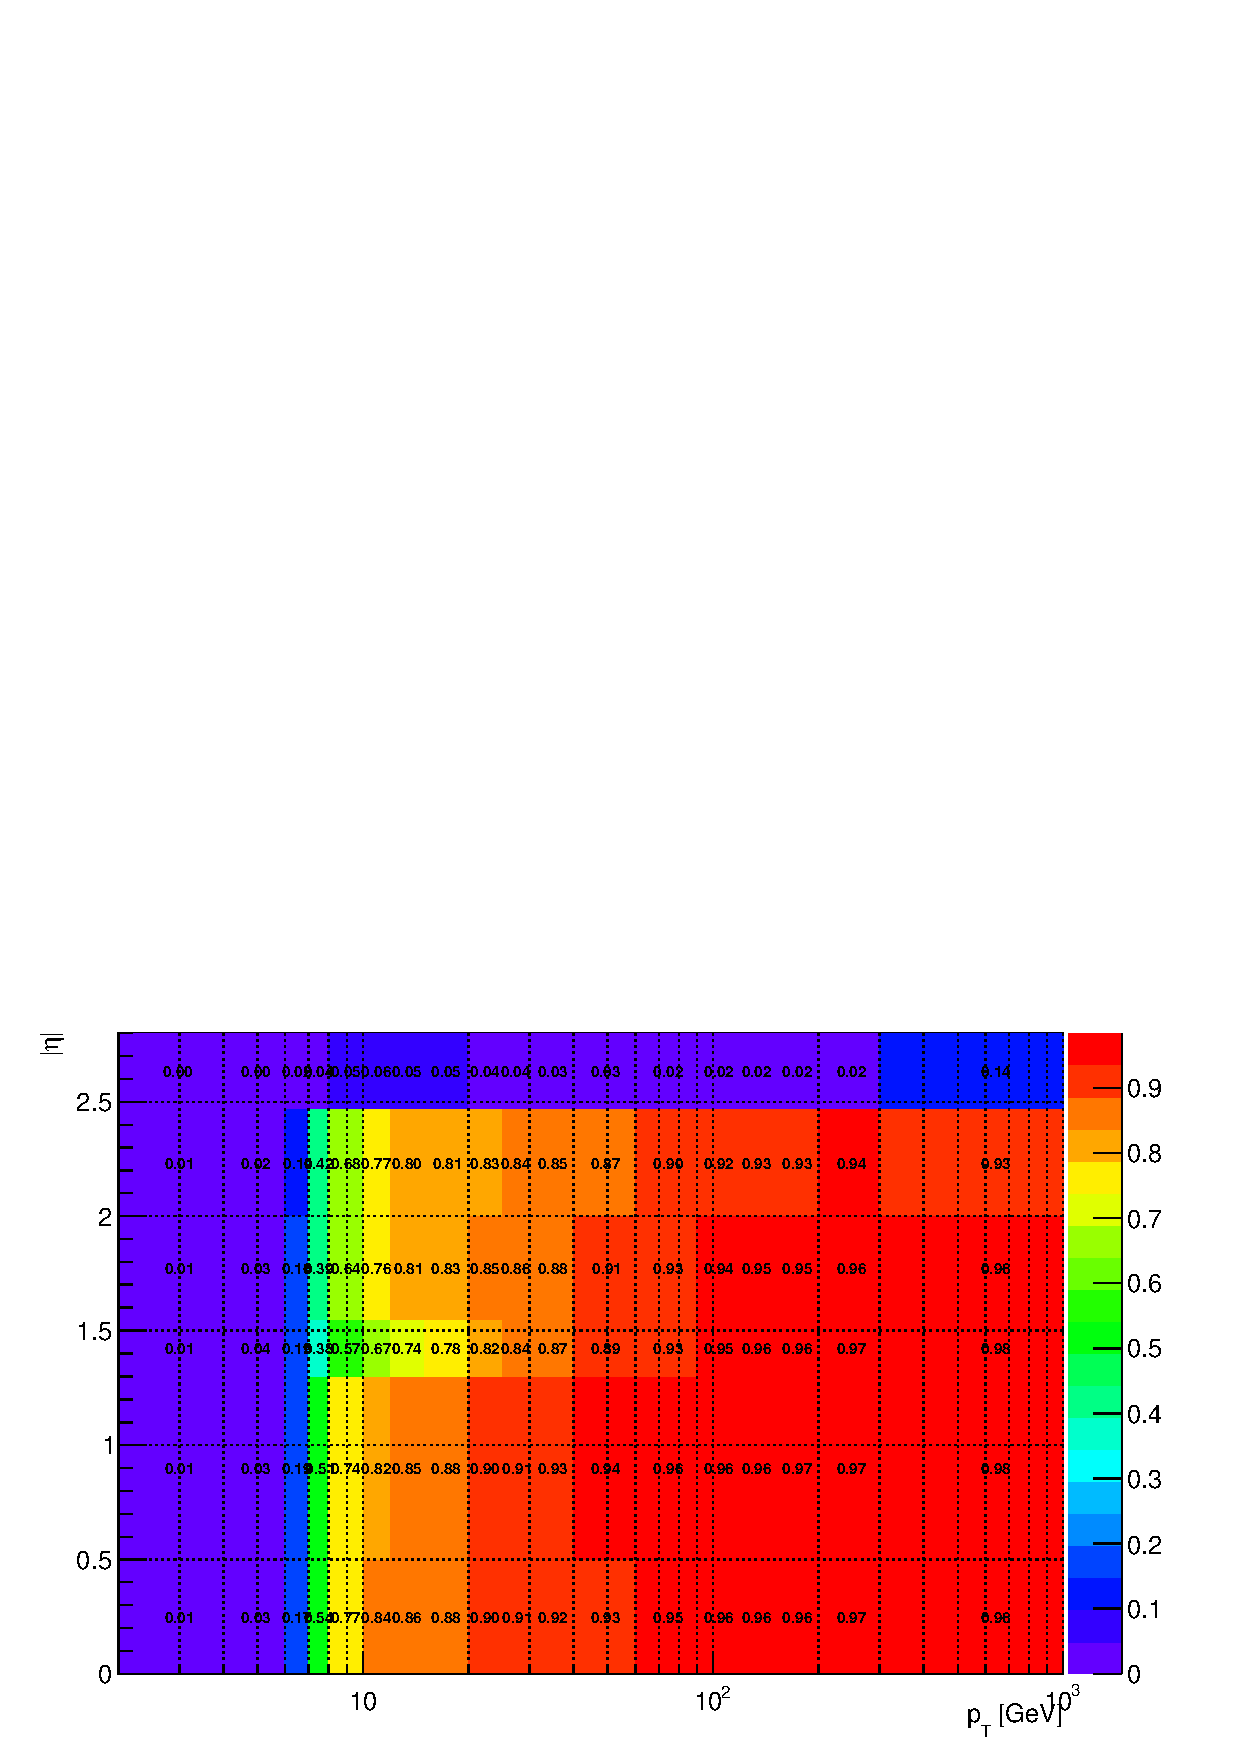
\includegraphics[width=75mm]{figures/BGestimation/ObjReplacement/method/lepeff/el_trPtEta_truthToID.pdf}
      \hspace{10mm} (a)
      \label{fig::ObjReaplce::heff_mc_el_truthToID}
    \end{minipage}
    \begin{minipage}[t]{.45\textwidth}
      \centering
      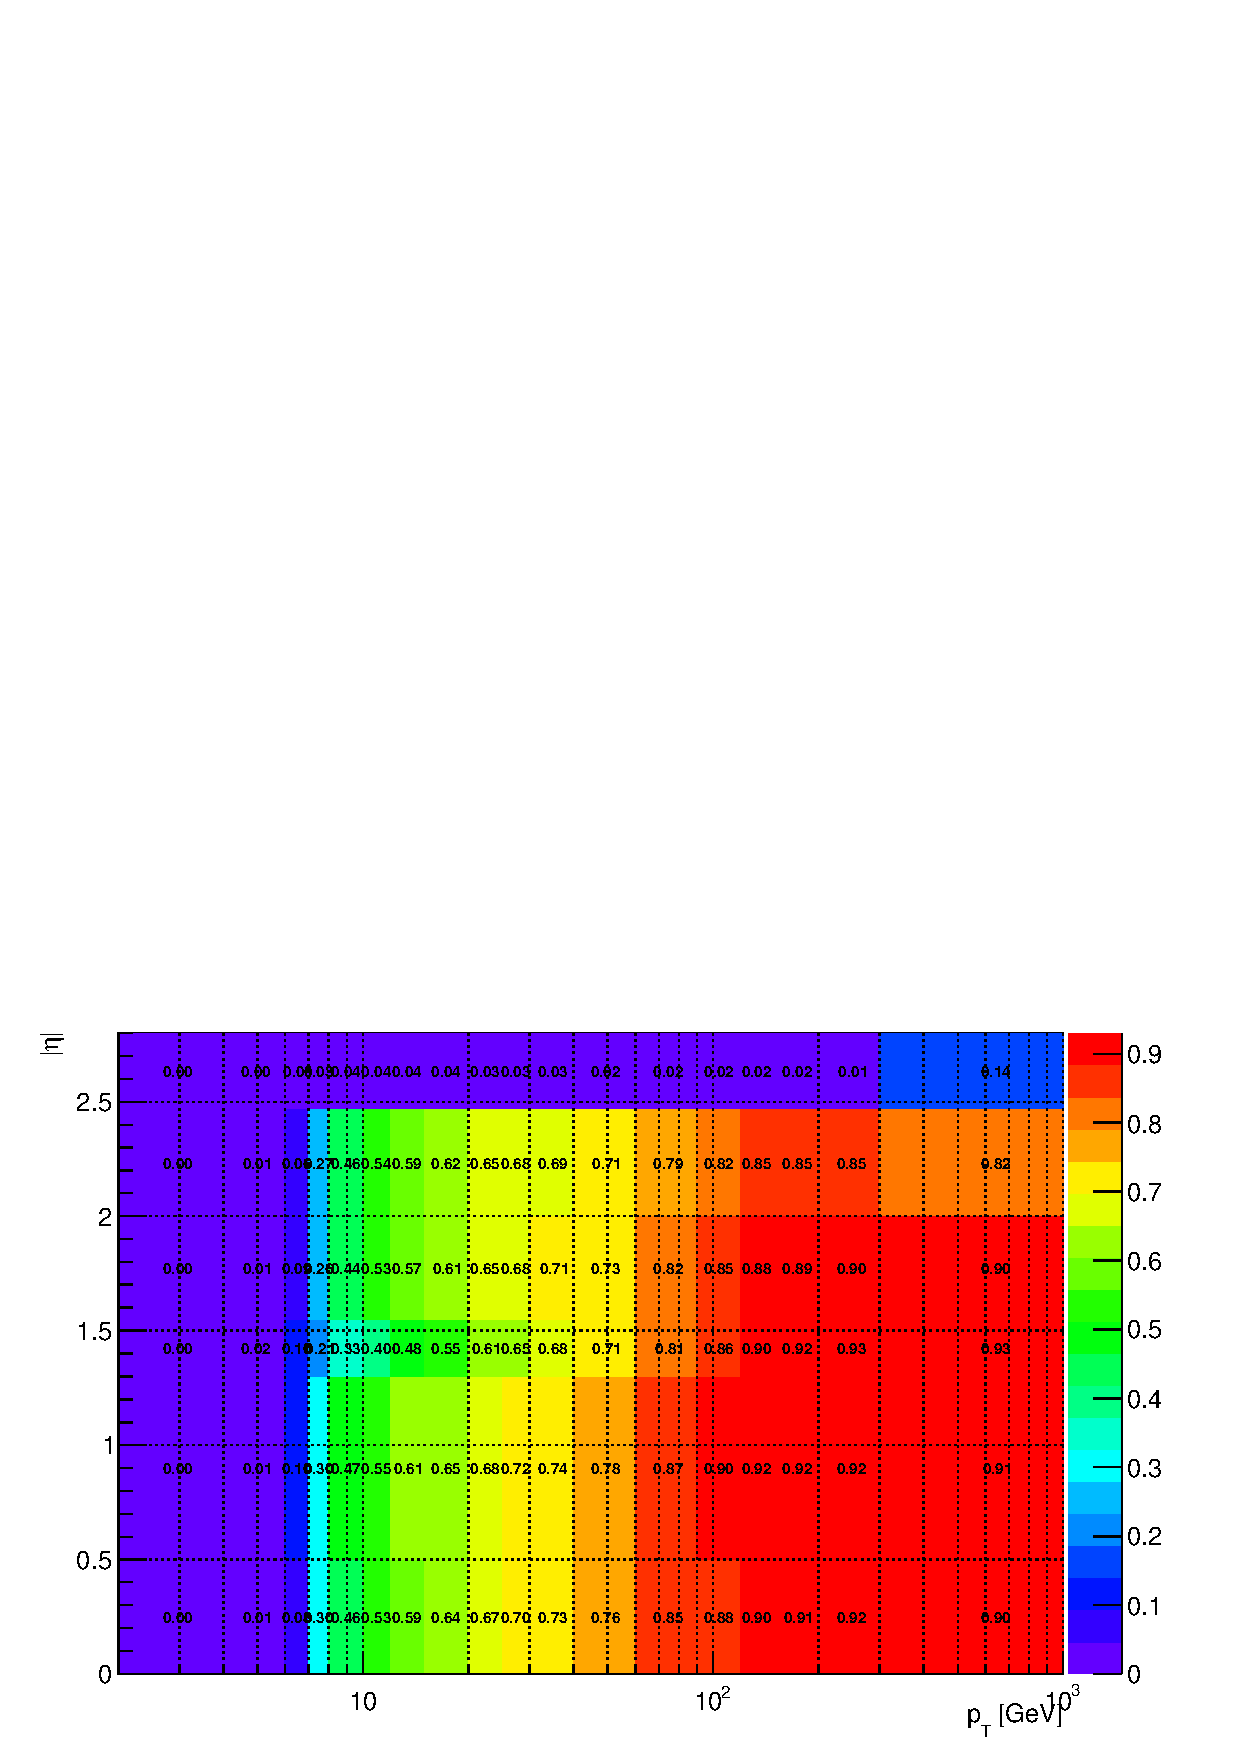
\includegraphics[width=75mm]{figures/BGestimation/ObjReplacement/method/lepeff/el_trPtEta_truthToSig.pdf}
      \hspace{10mm} (b)
      \label{fig::ObjReaplce::heff_mc_el_truthToSig}
    \end{minipage}
    %
    \begin{minipage}[t]{.45\textwidth}
      \centering
      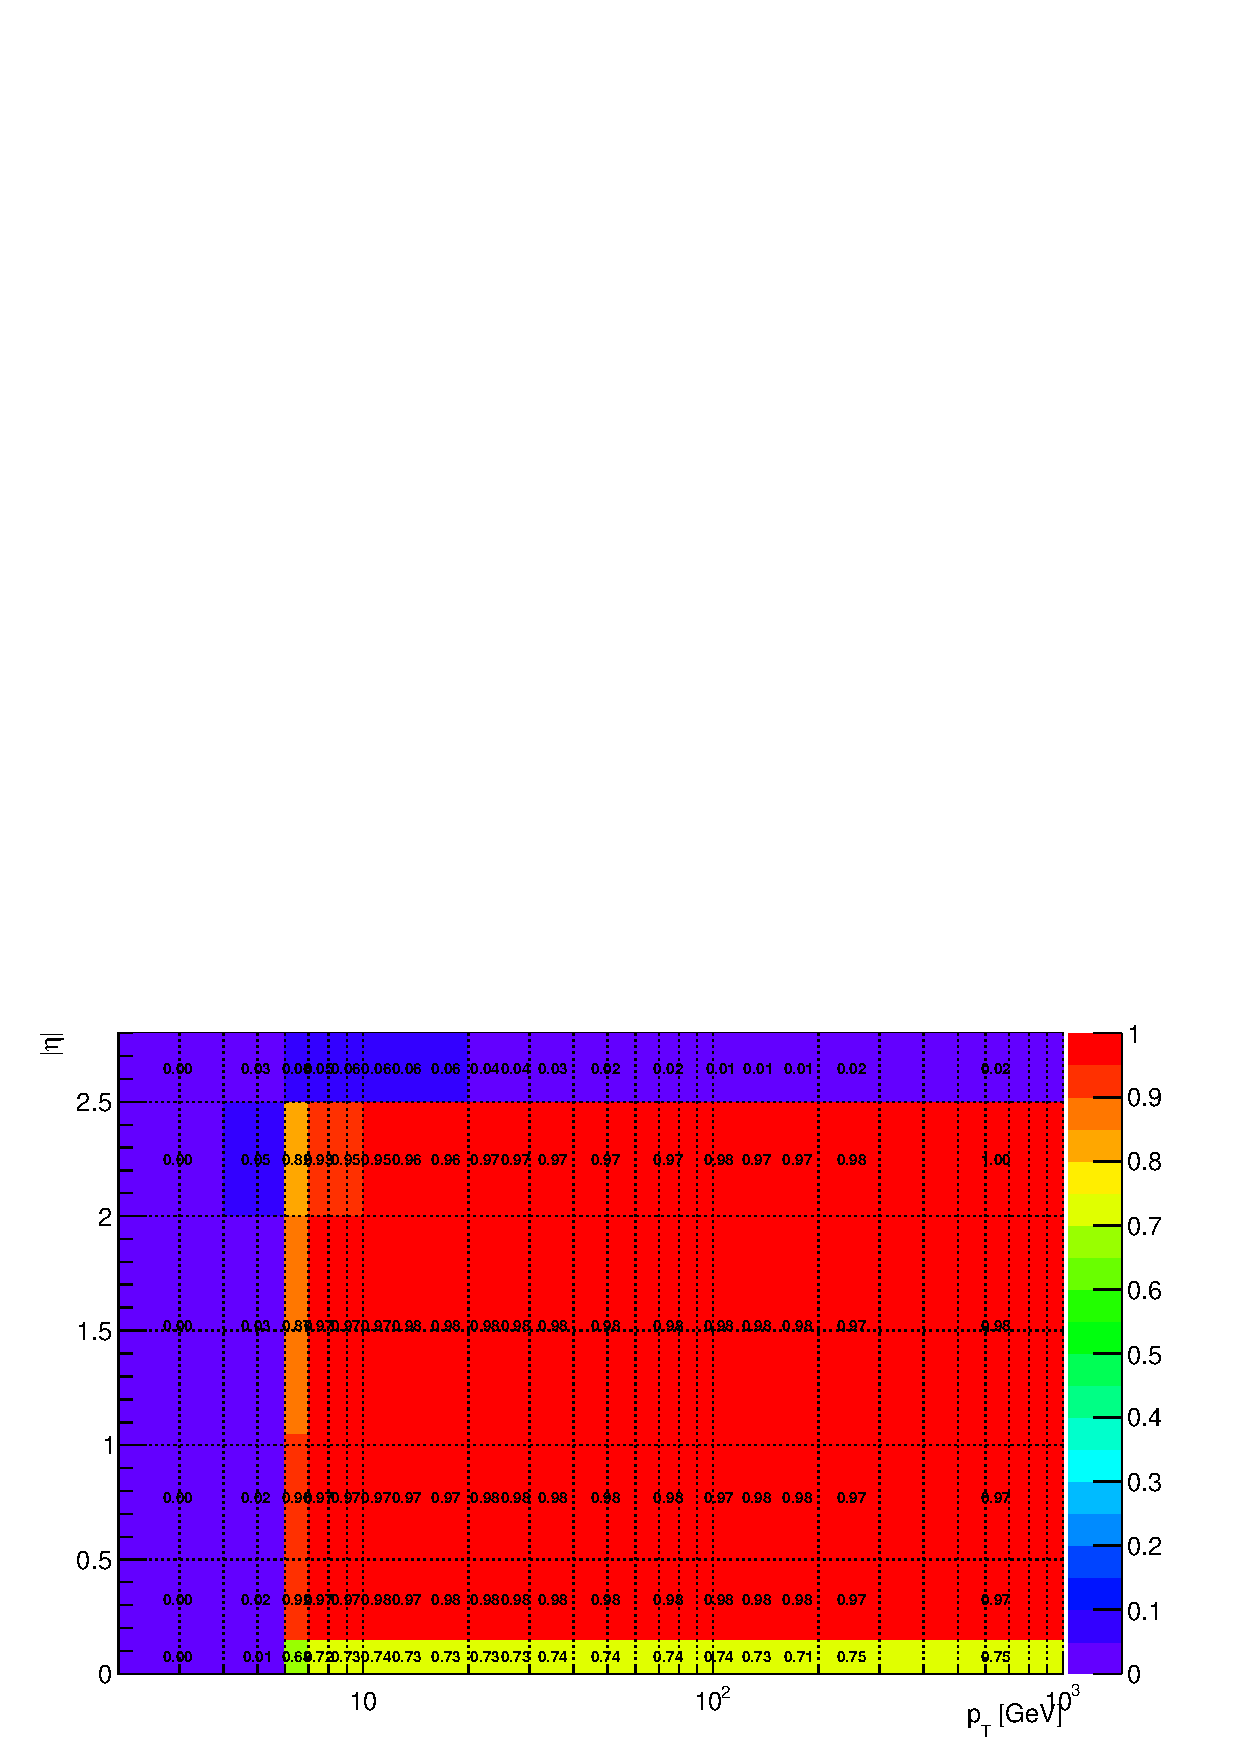
\includegraphics[width=75mm]{figures/BGestimation/ObjReplacement/method/lepeff/mu_trPtEta_truthToID.pdf}
      \hspace{10mm} (c)
      \label{fig::ObjReaplce::heff_mc_mu_truthToID}
    \end{minipage}
    \begin{minipage}[t]{.45\textwidth}
      \centering
      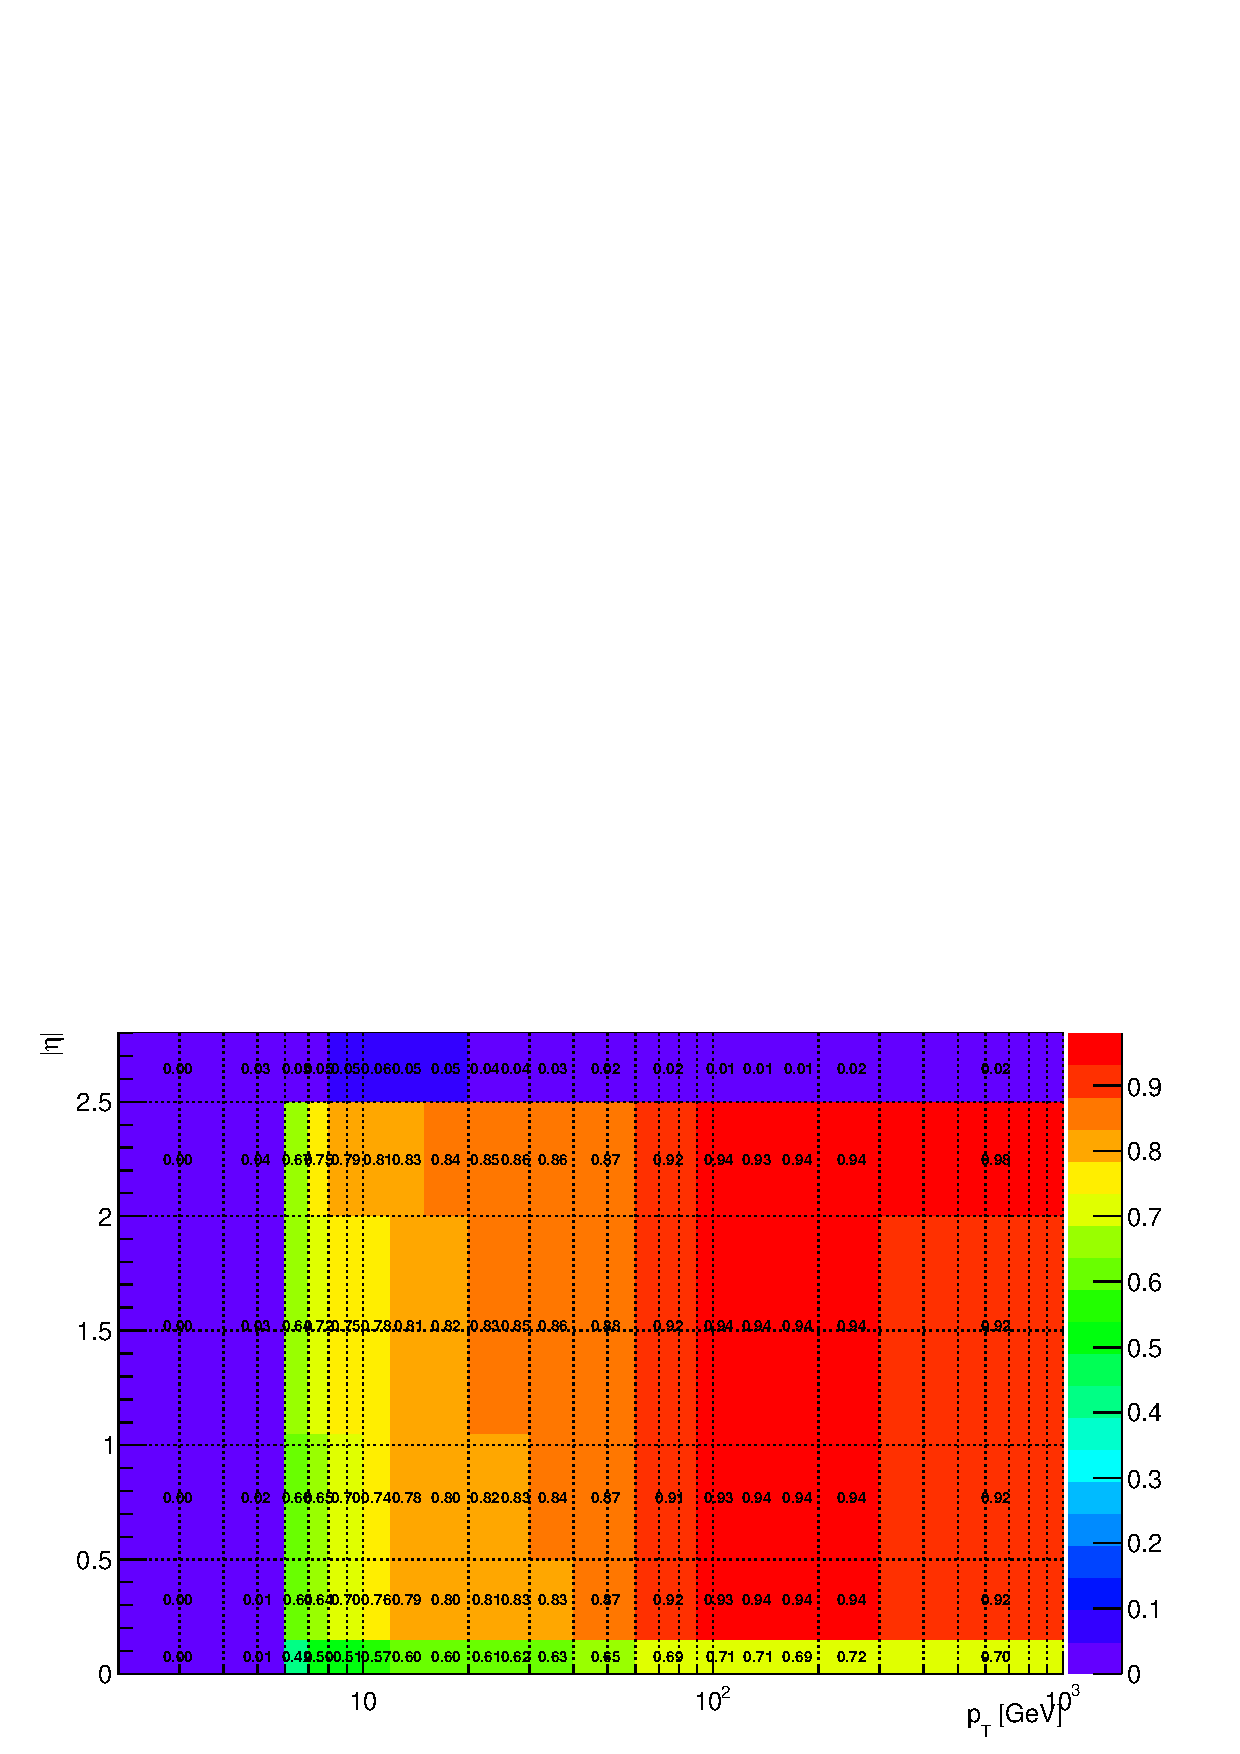
\includegraphics[width=75mm]{figures/BGestimation/ObjReplacement/method/lepeff/mu_trPtEta_truthToSig.pdf}
      \hspace{10mm} (d)
      \label{fig::ObjReaplce::heff_mc_mu_truthToSig}
    \end{minipage}
    %
    \caption{Off-line selection efficiency used in transfer factor calulation. (a) Efficiency of electrons passing reconstruction and ID. (b) Efficiency of electrons passing signal lepton requirement.  (c) Efficiency of muons passing reconstruction and ID. (d) Efficiency of muons passing signal lepton requirement.}
    \label{fig::ObjReaplce::lep_efficiency}
  \end{center}
\end{figure}



%%%%%%%%%%%%%%%%%%%%%%%%%% MC Closure test %%%%%%%%%%%%%%%%%%%%%%%%%%%%%%%%
\clearpage
\subsection{Closure Test using $t\bar{t}$ MC Samples} \label{sec::ObjReplace::mcClosure}
%
\subsubsection{Closuer test with loose selection.} \label{sec::ObjReplace::mcClosure_loose} 
The methodologies are tested by comparing yields and distributions between the estimation by object replacement and the actual $\ell\ell_{\mathrm{mis.}}$/$\ell\tau_{\mathrm{h}}$ events, in a region with exactly one baseline lepton (``Closure test''), using the Powheg+Pythia6 $t\bar{t}$ MC. The level of disagreement (non-closure) indicates the generic accuracy about this method, which will be quoted as systematics. Fig.\ref{fig::ObjReplace::mcClosure_MisLep_el} $\sim$ \ref{fig::ObjReplace::mcClosure_TauRep_emu} show the result for the hard lepton regions and fig.\ref{fig::ObjReplace::mcClosure_softLep_MisLep_el} $\sim$ \ref{fig::ObjReplace::mcClosure_softLep_TauRep_emu} are for the soft lepton regions. MET cut for the seed selection is removed for the hard lepton case in order to boost the statistics enought to test the shape. The other selections follow tab.\ref{tab::ObjReplace::method::2LCR}.

% ---------- mcClosure::plot::hardLep
%%%%% METHNAME %%%%%%%%%%%%%%%%%%%%%%%%%%
\begin{figure}[h]
  \centering
    \subfigure[]{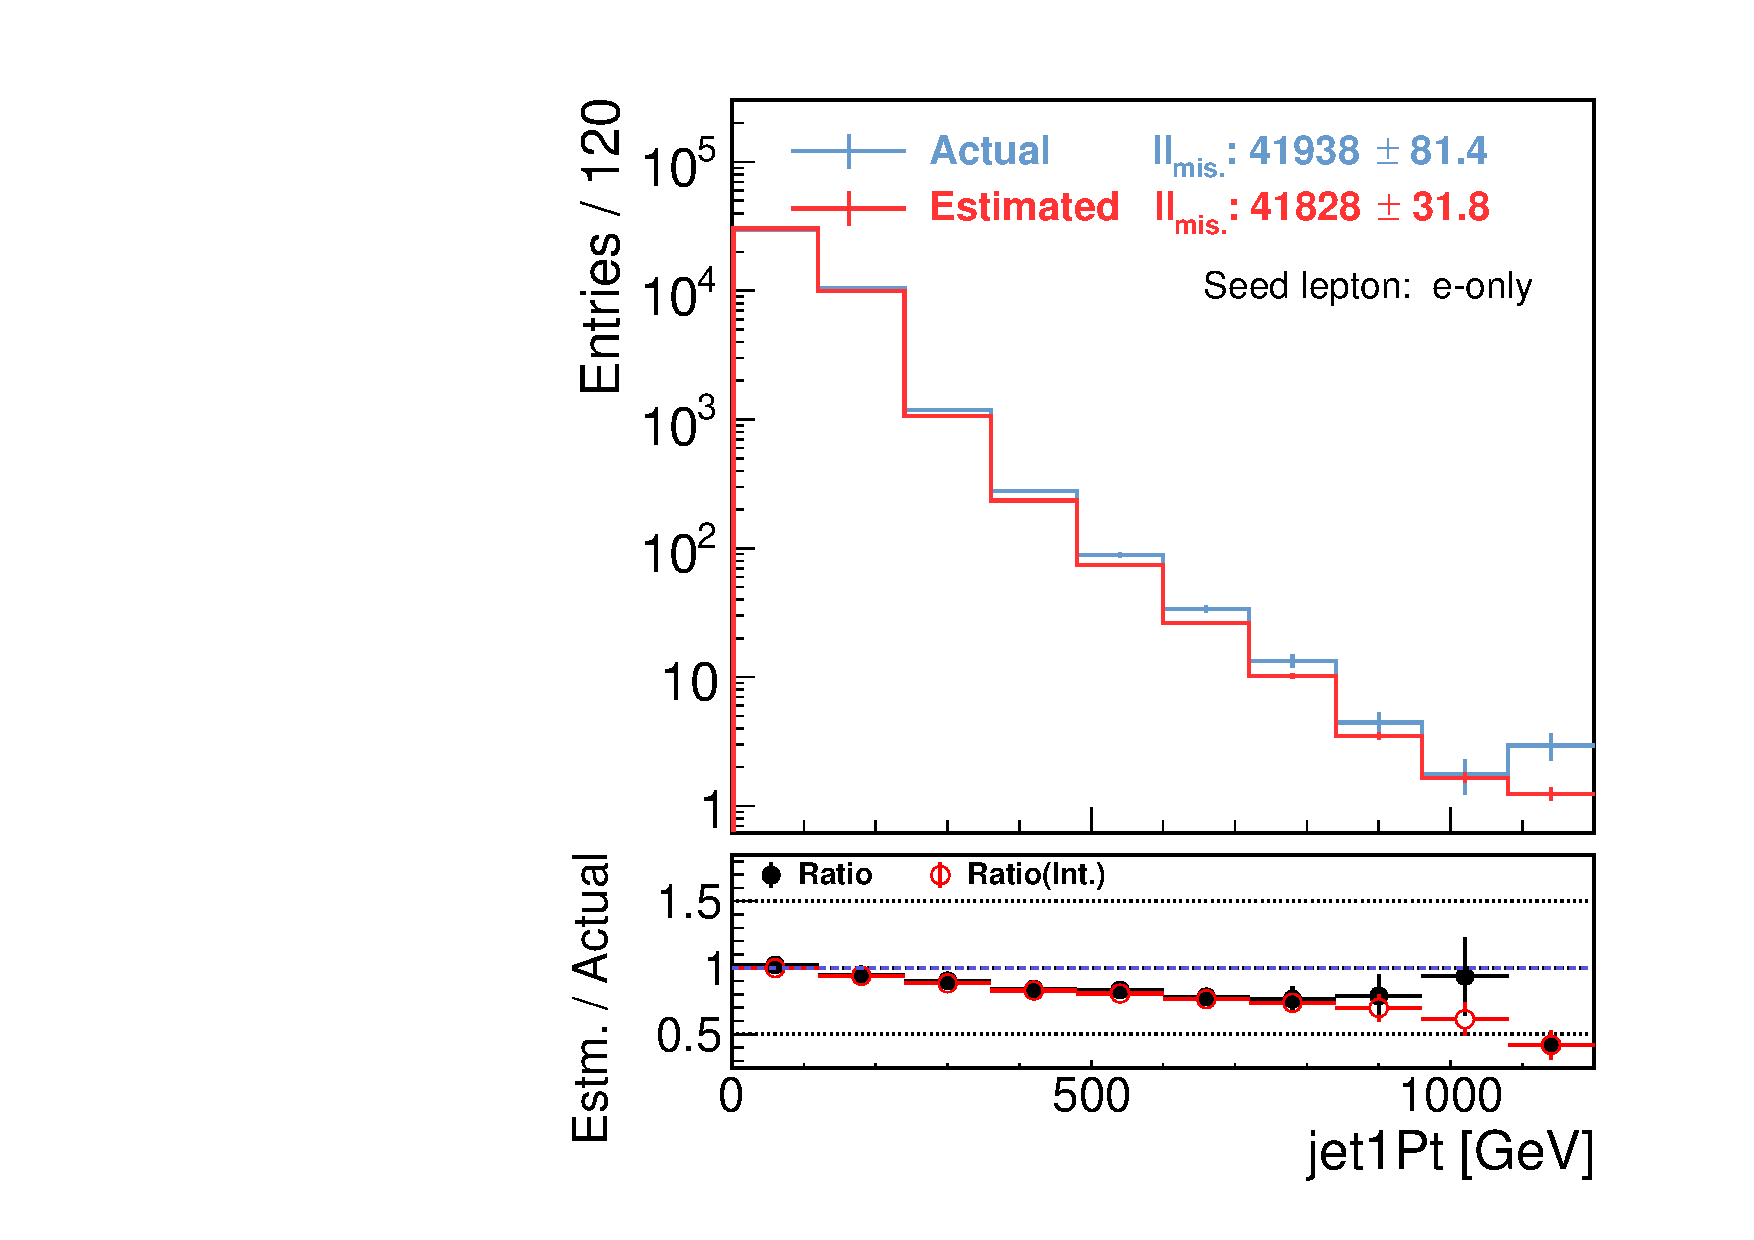
\includegraphics[width=0.32\textwidth]{figures/BGestimation/ObjReplacement/mcClosure/MisLep_el/MisLep_el_jet1Pt__trMode4_NoSys.pdf}}
    \subfigure[]{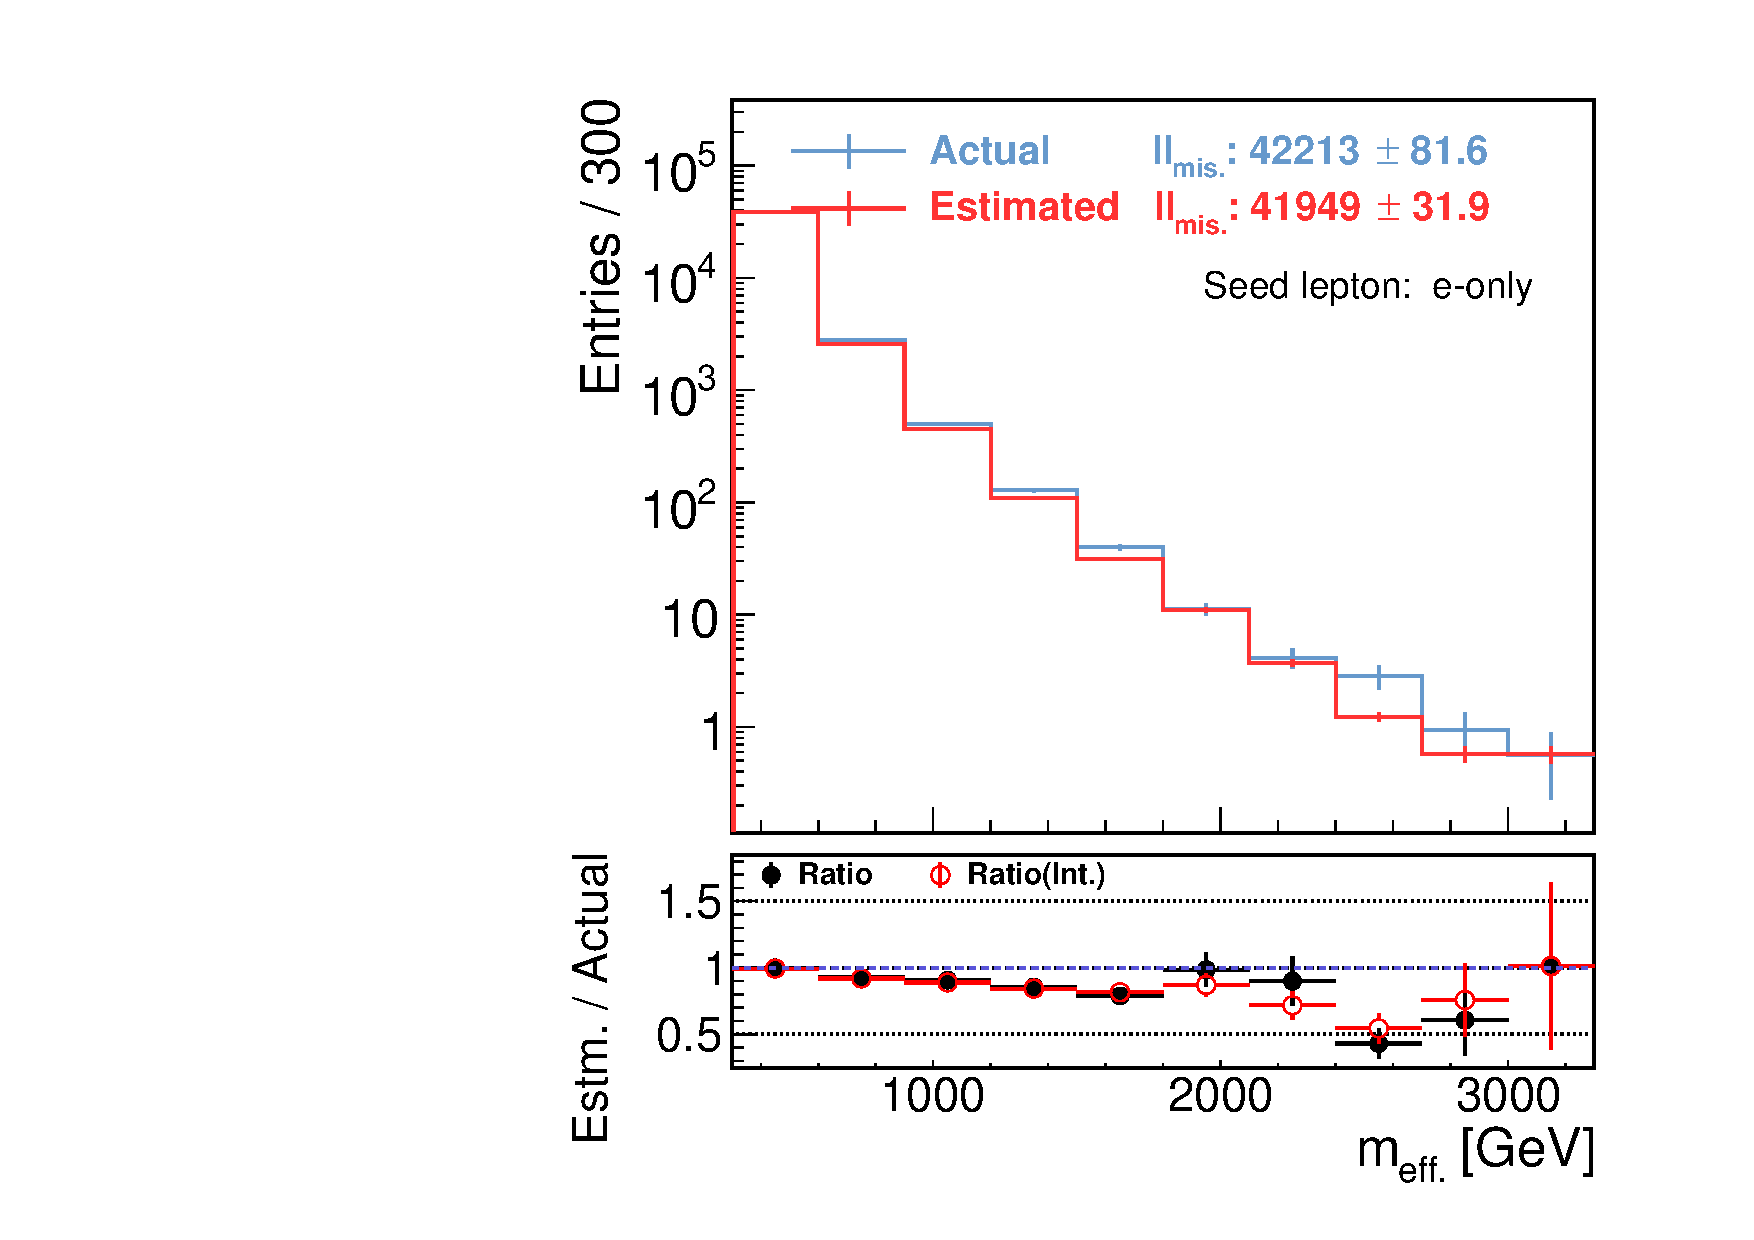
\includegraphics[width=0.32\textwidth]{figures/BGestimation/ObjReplacement/mcClosure/MisLep_el/MisLep_el_meffInc30__trMode4_NoSys.pdf}}
    \subfigure[]{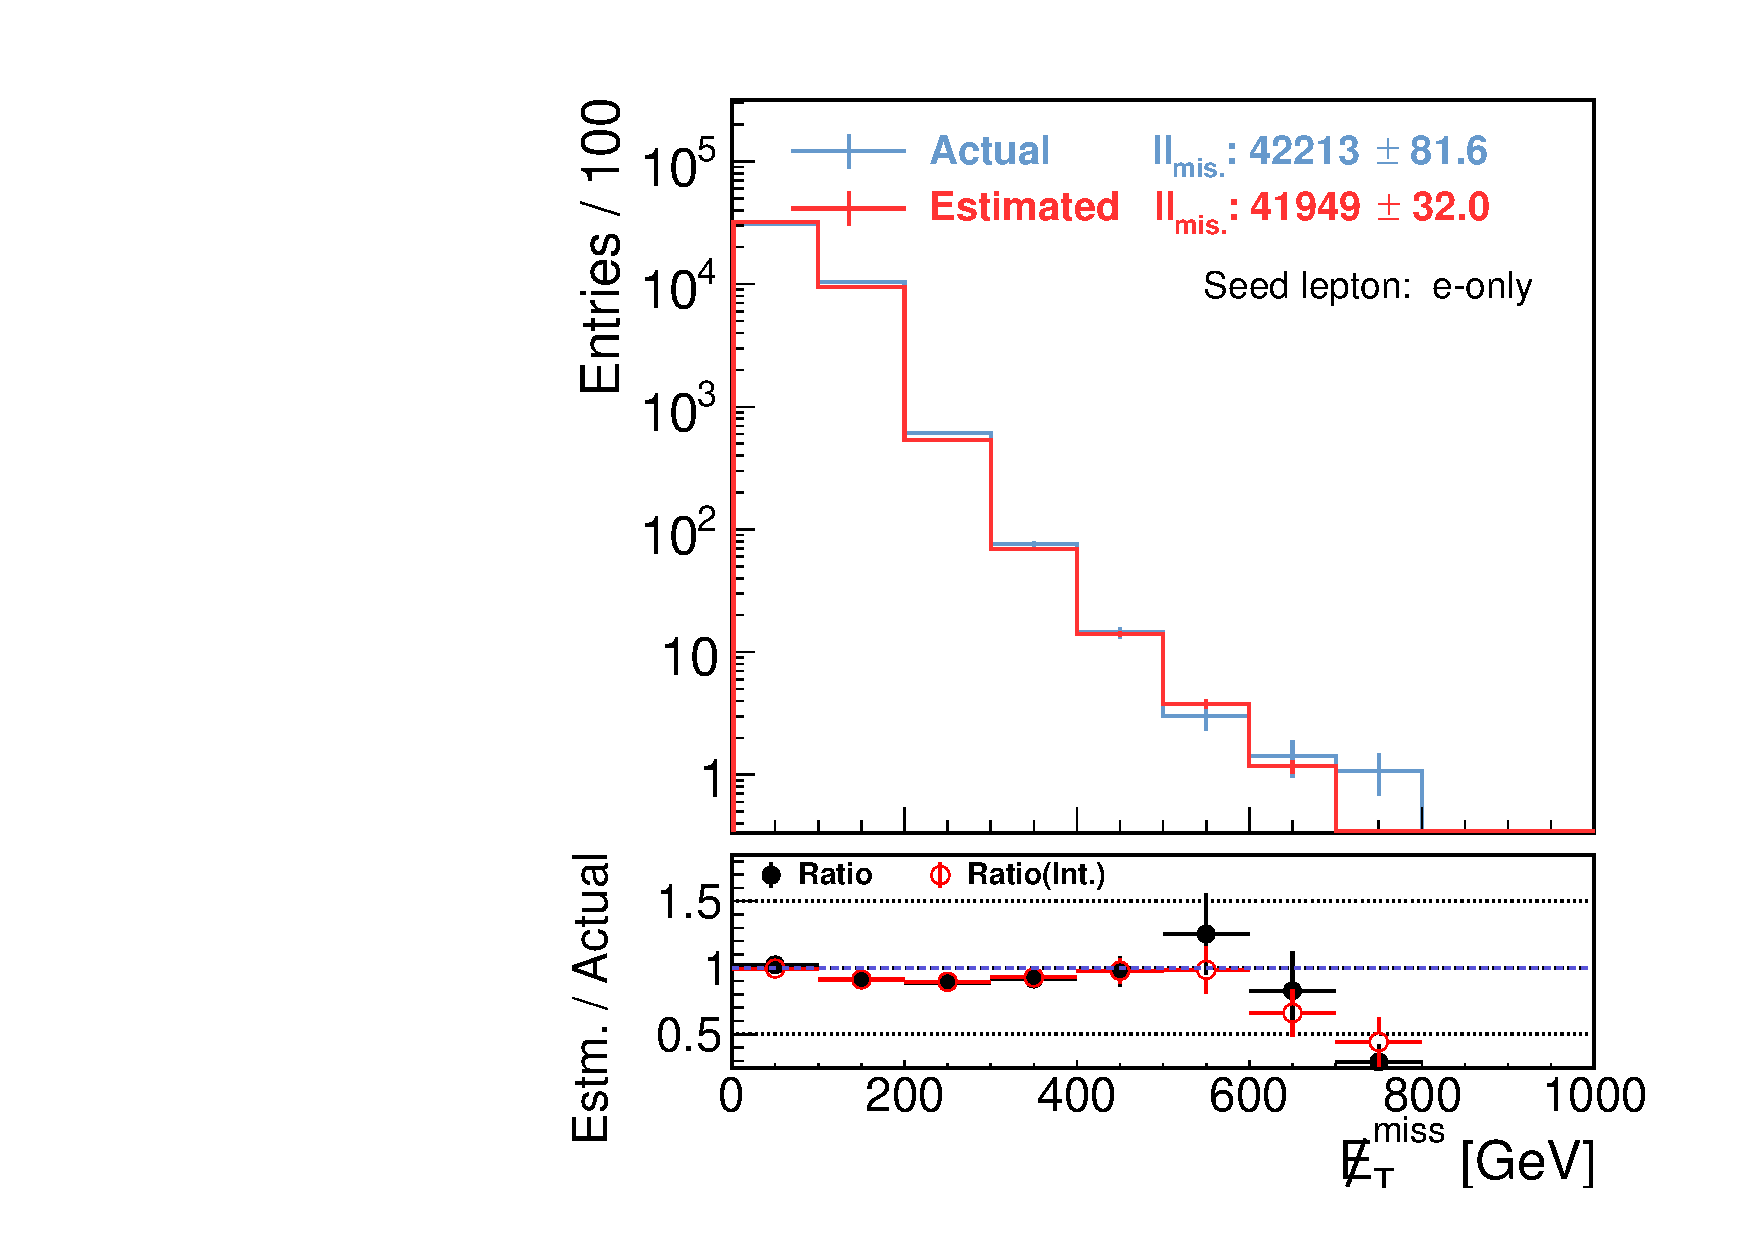
\includegraphics[width=0.32\textwidth]{figures/BGestimation/ObjReplacement/mcClosure/MisLep_el/MisLep_el_met__trMode4_NoSys.pdf}}
    \subfigure[]{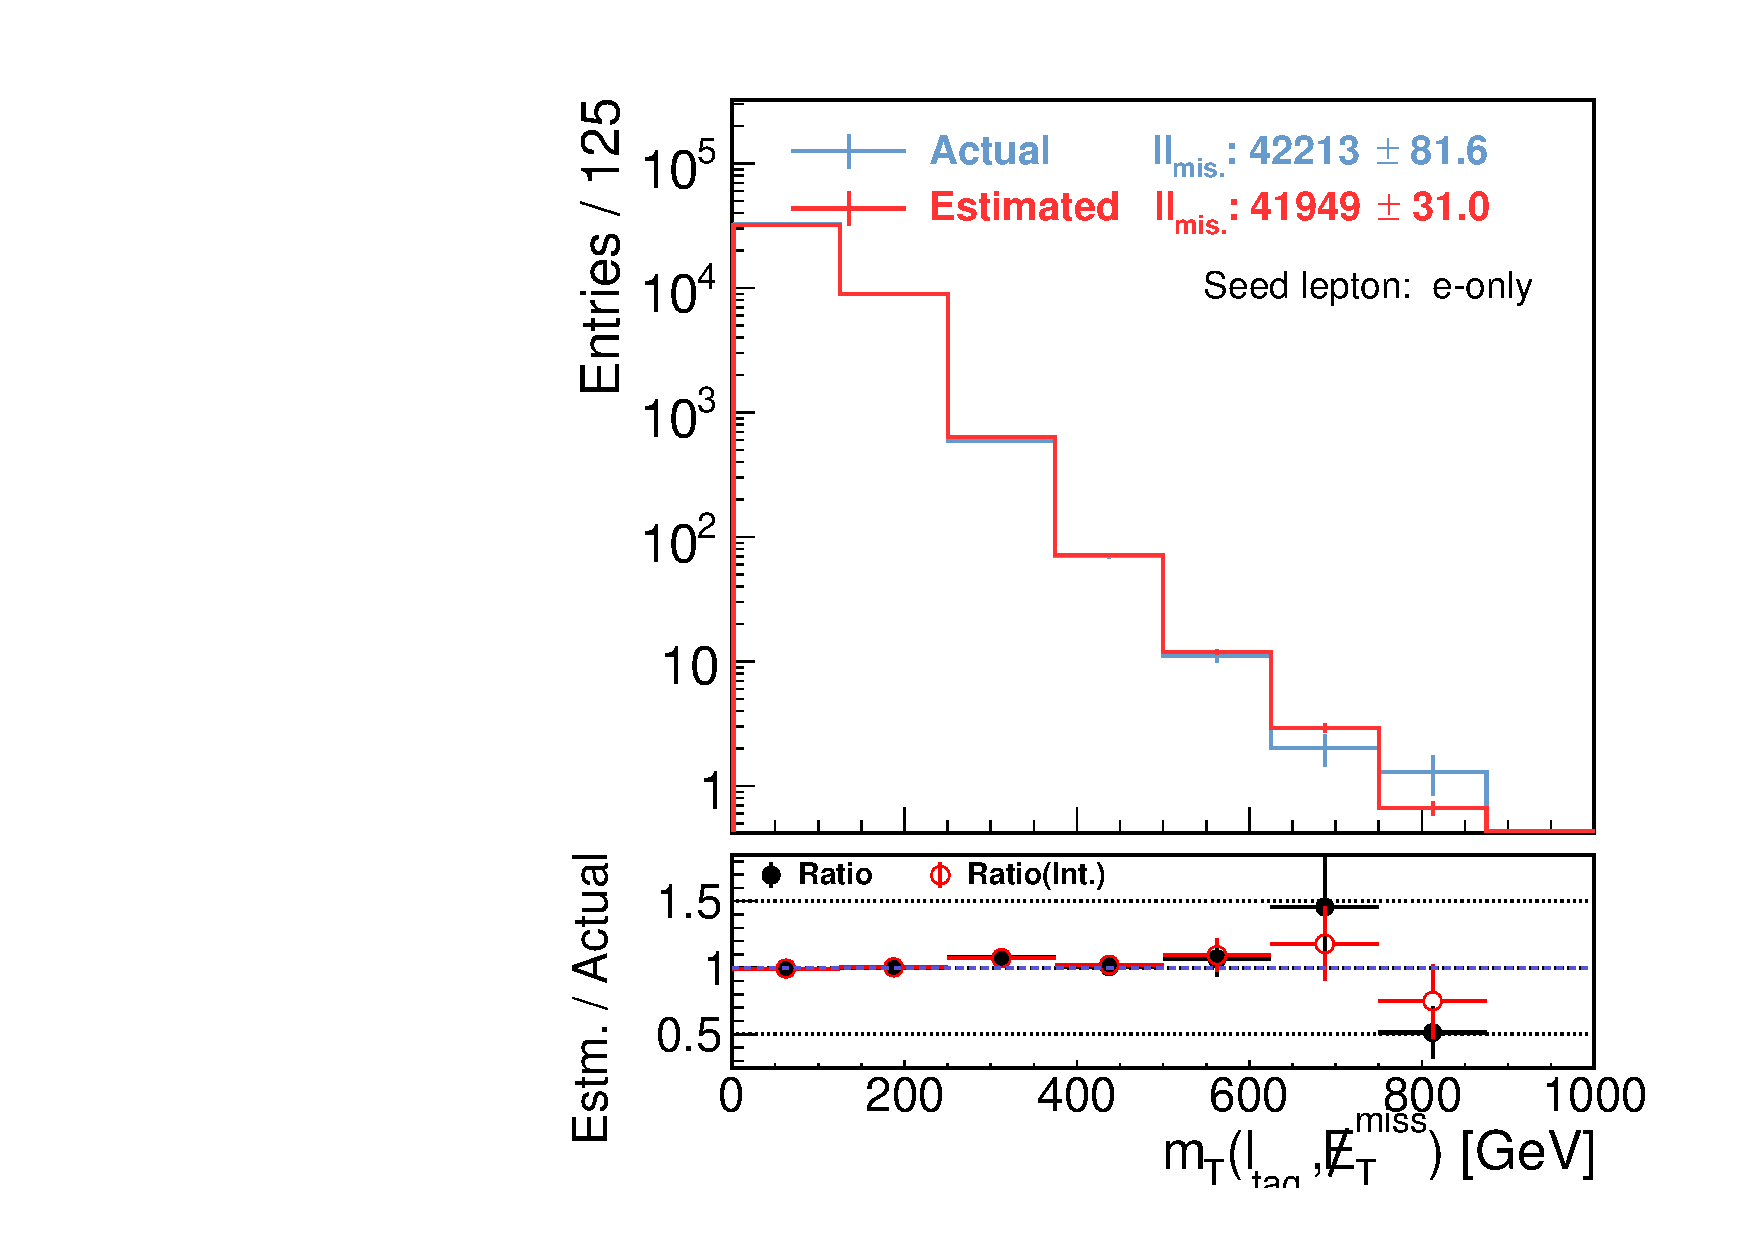
\includegraphics[width=0.32\textwidth]{figures/BGestimation/ObjReplacement/mcClosure/MisLep_el/MisLep_el_mt__trMode4_NoSys.pdf}}
    \subfigure[]{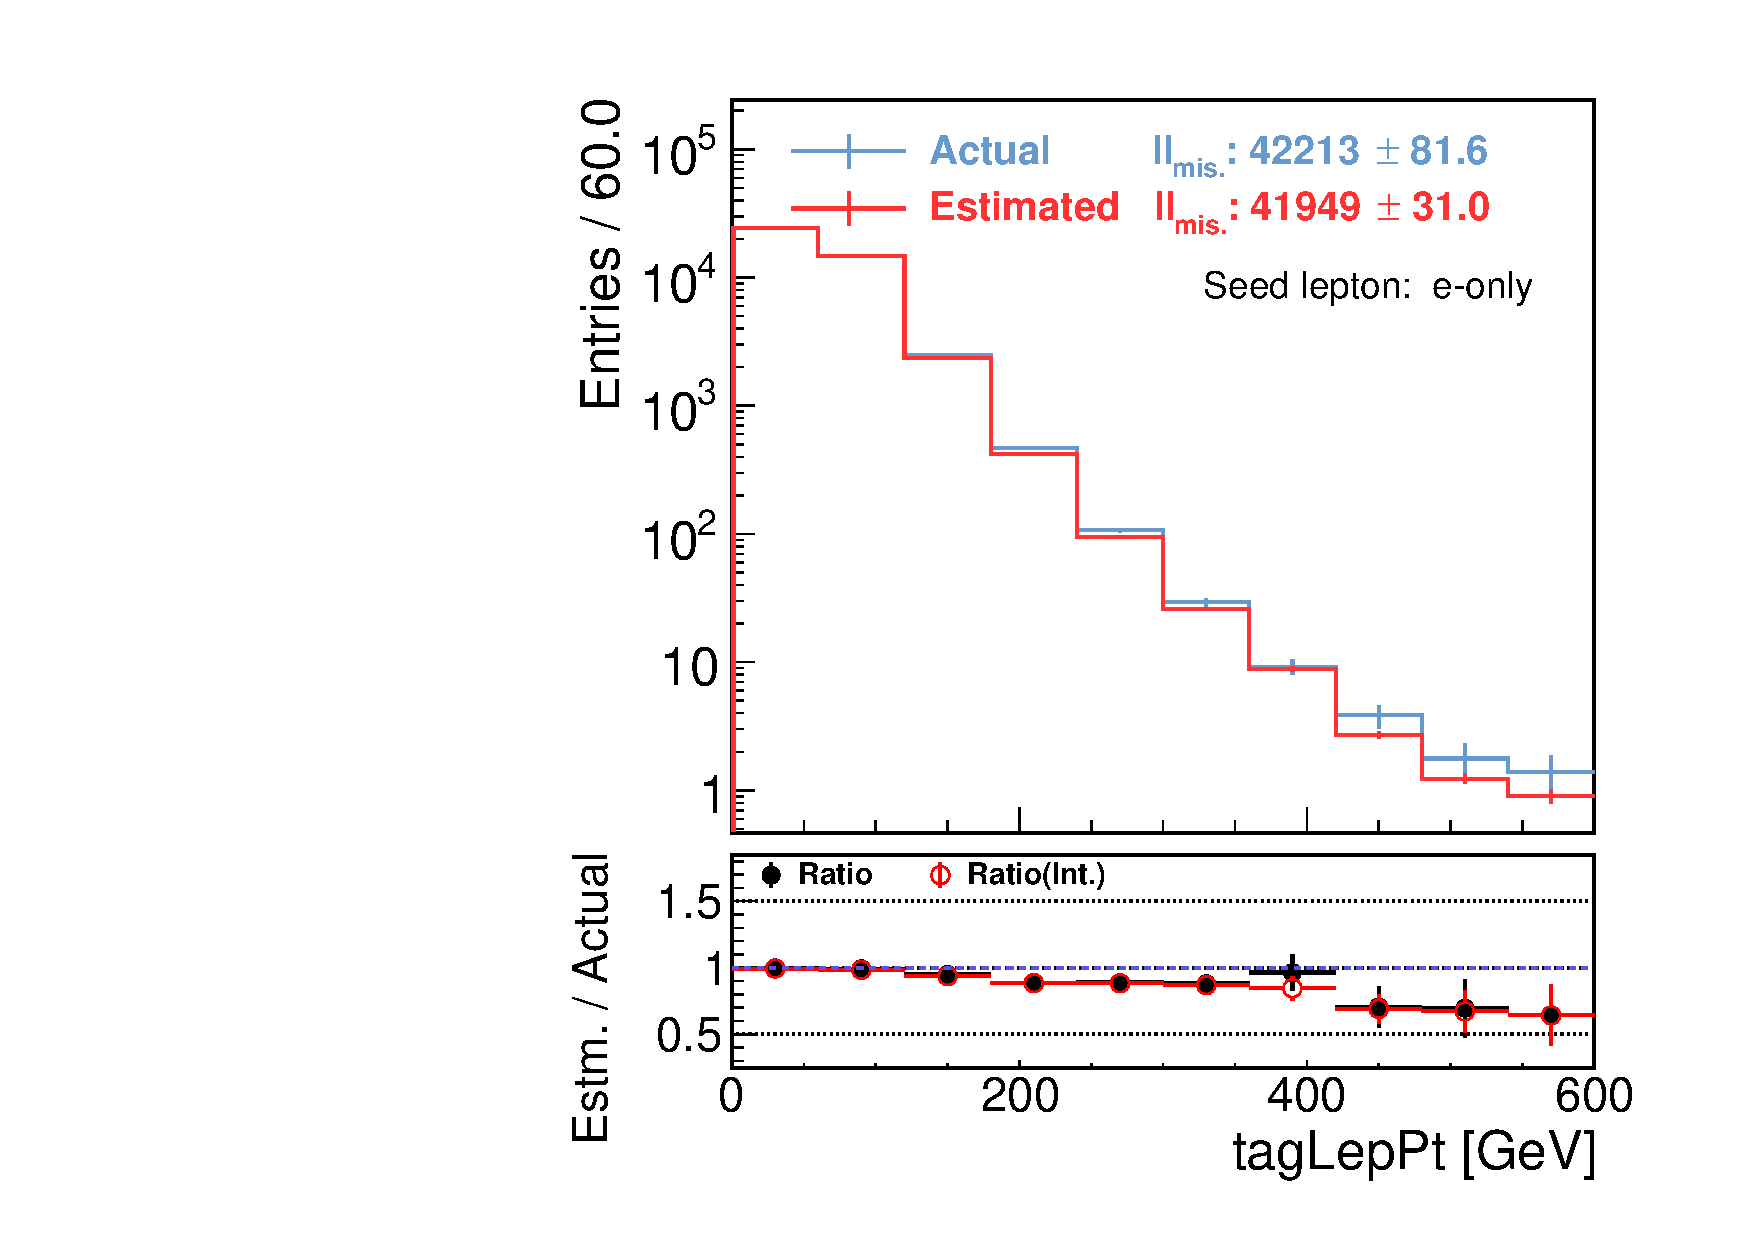
\includegraphics[width=0.32\textwidth]{figures/BGestimation/ObjReplacement/mcClosure/MisLep_el/MisLep_el_tagLepPt__trMode4_NoSys.pdf}}
    \subfigure[]{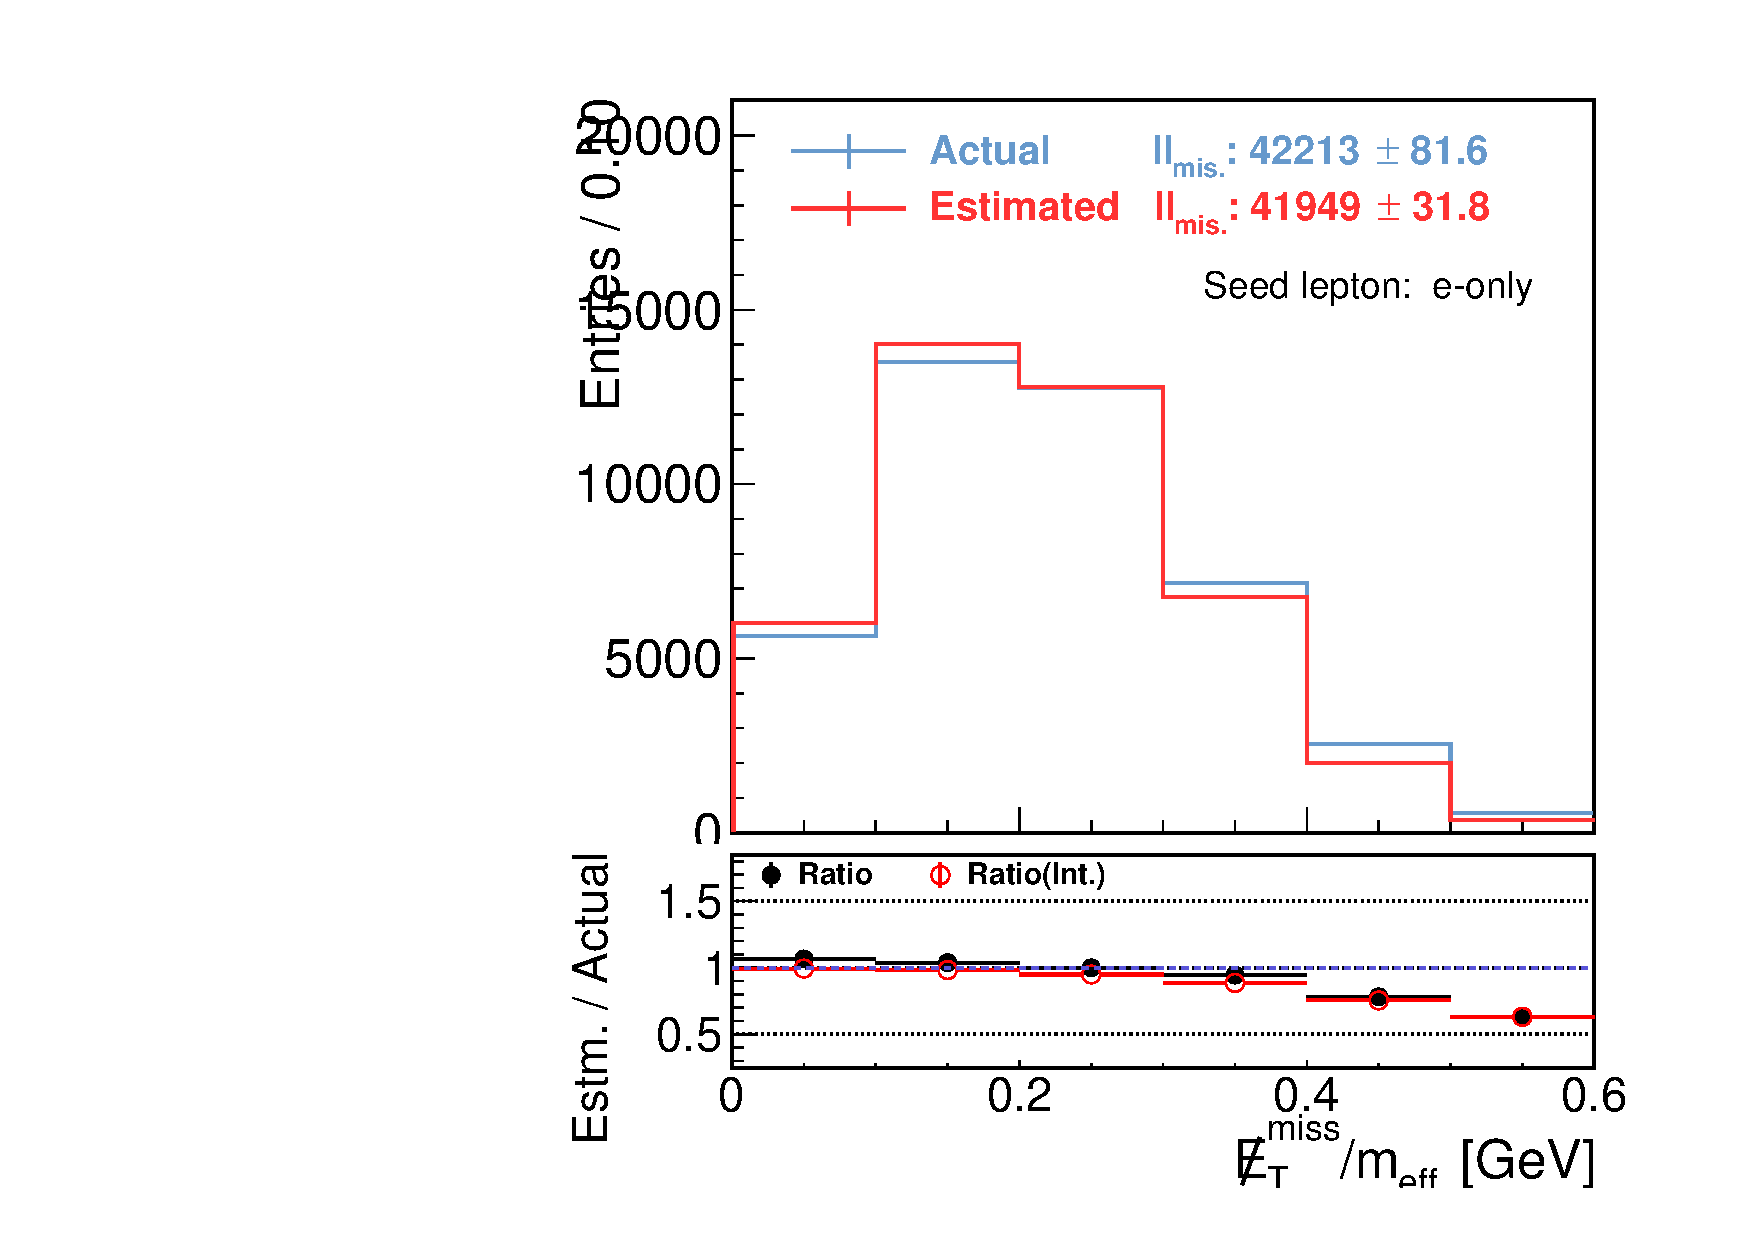
\includegraphics[width=0.32\textwidth]{figures/BGestimation/ObjReplacement/mcClosure/MisLep_el/MisLep_el_metOverMeff__trMode4_NoSys.pdf}}
    \subfigure[]{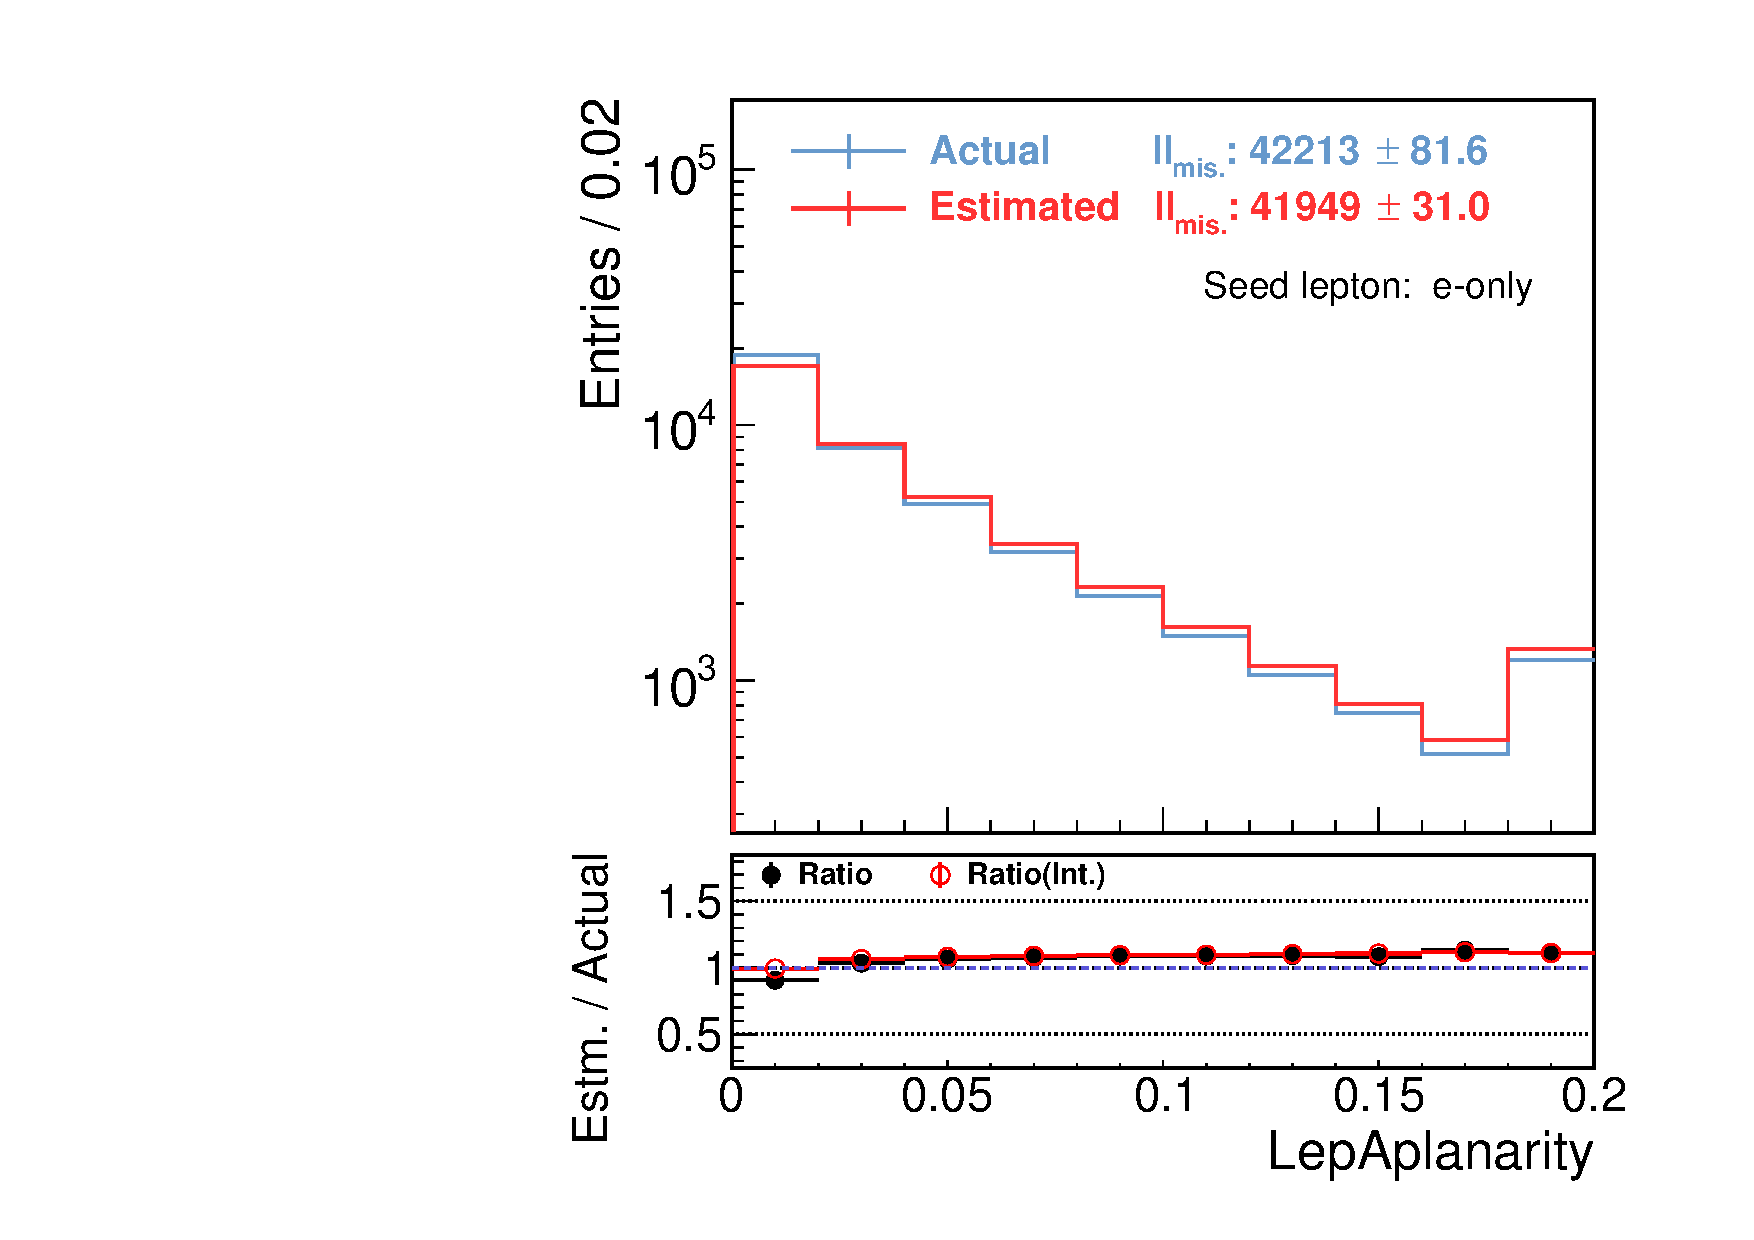
\includegraphics[width=0.32\textwidth]{figures/BGestimation/ObjReplacement/mcClosure/MisLep_el/MisLep_el_LepAplanarity__trMode4_NoSys.pdf}}
    \subfigure[]{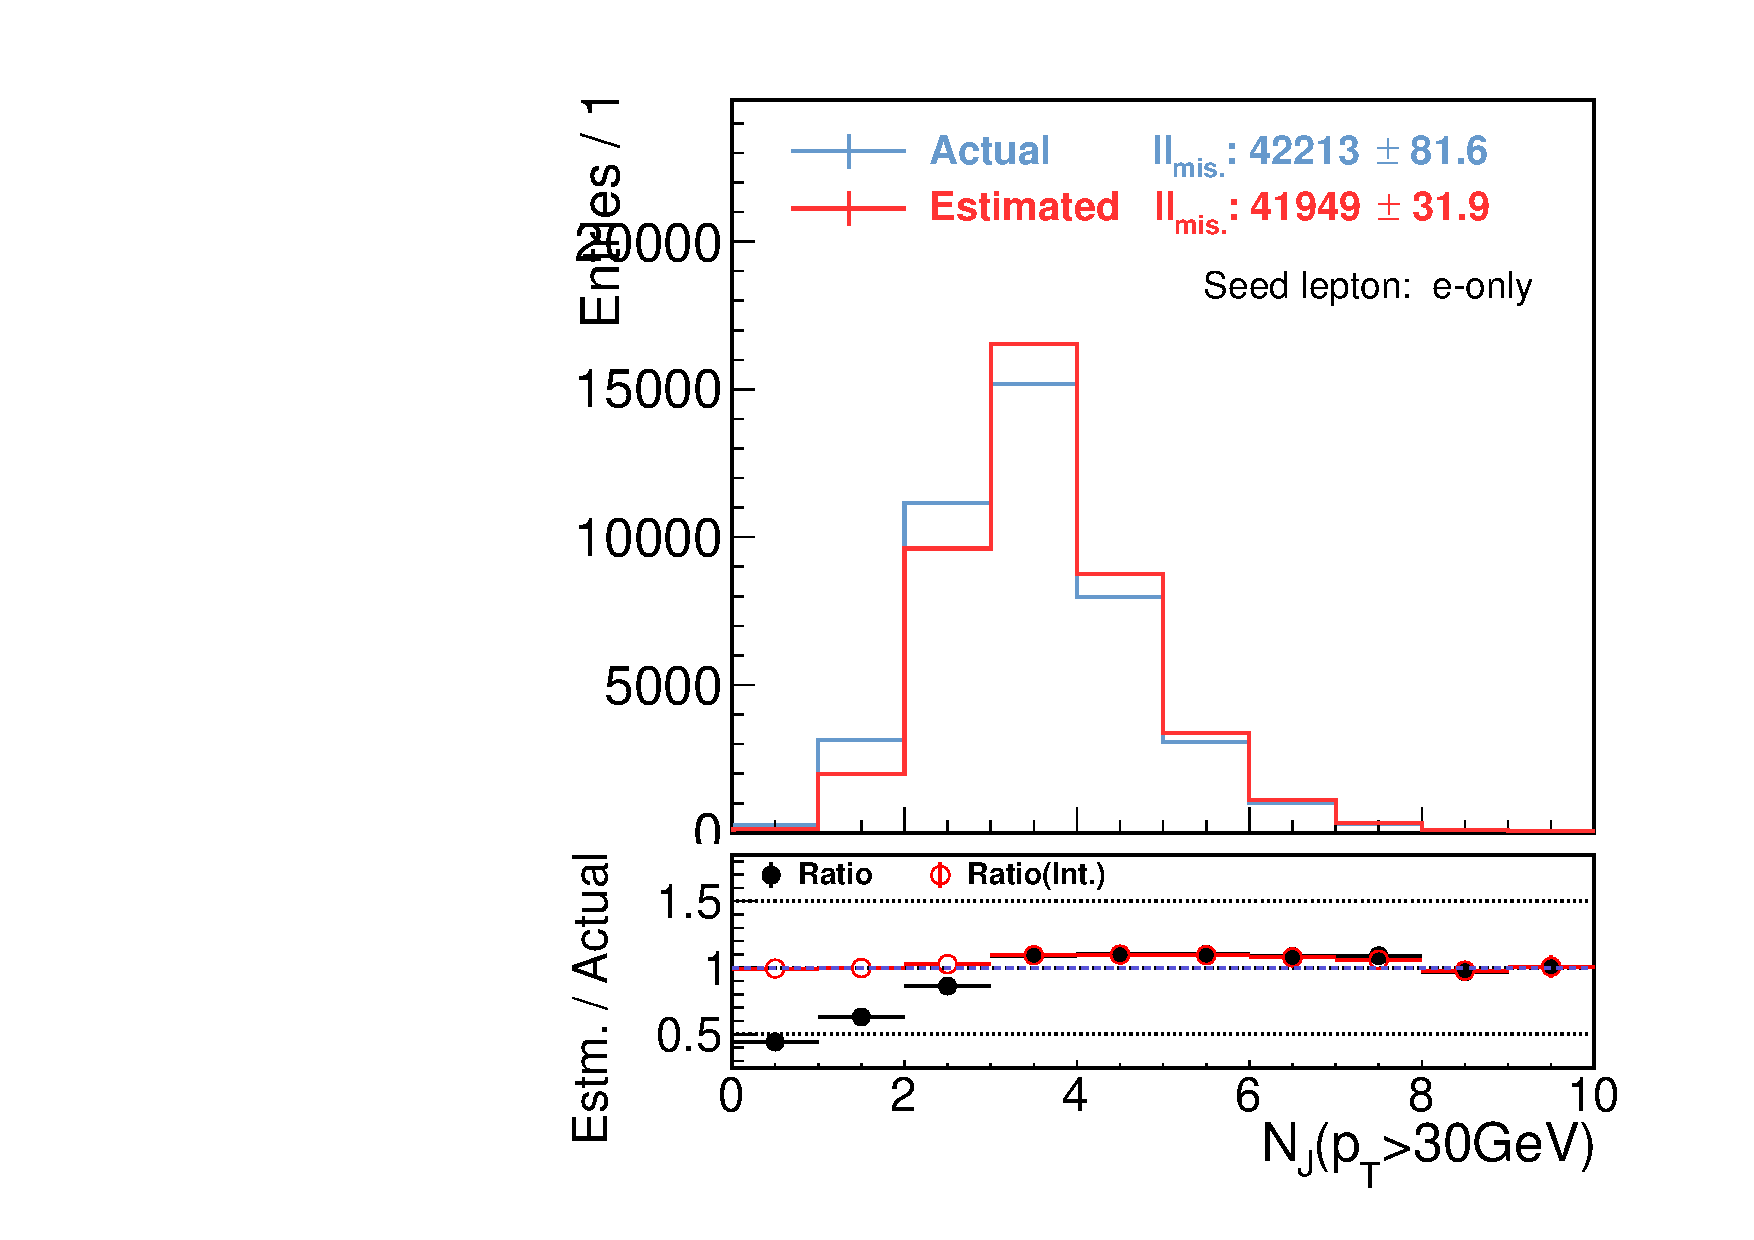
\includegraphics[width=0.32\textwidth]{figures/BGestimation/ObjReplacement/mcClosure/MisLep_el/MisLep_el_nJet30__trMode4_NoSys.pdf}}
    \subfigure[]{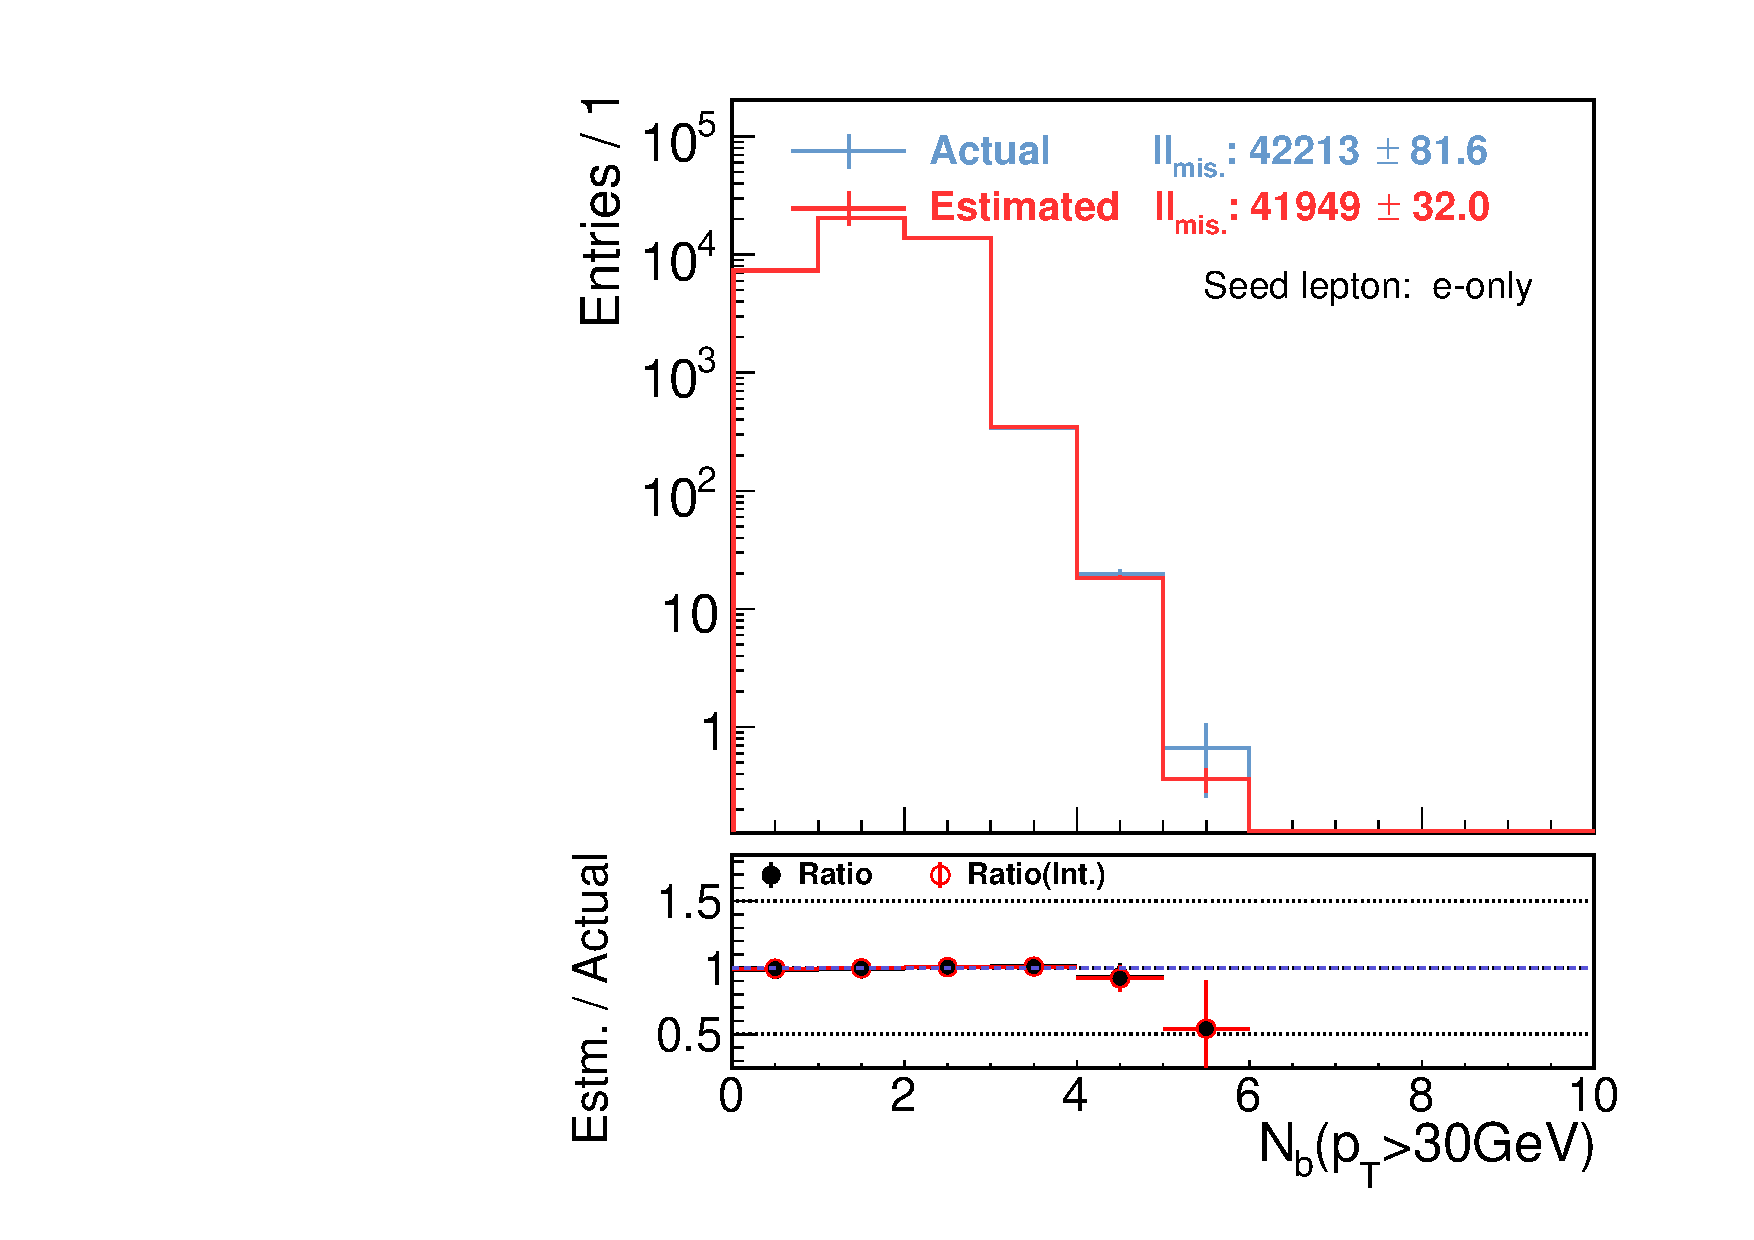
\includegraphics[width=0.32\textwidth]{figures/BGestimation/ObjReplacement/mcClosure/MisLep_el/MisLep_el_nBJet30__trMode4_NoSys.pdf}}
    \caption{ MC closure test for \textbf{missing lepton replacement} using $t\bar{t}$ MC sample. Seed events are collected by the single-lepton trigger. $p_T>35\gev$ for the leading lepton is required. \textbf{Only electrons in the seed events are replaced}. Red points in the bottom plots show the ratio of integrated yields for the two histograms above the x-position that the point indicates. \label{fig::ObjReplace::mcClosure_MisLep_el} }
\end{figure}
 %%%%%%%%%%%%%%%%%%%%%%%%%%

%%%%% METHNAME %%%%%%%%%%%%%%%%%%%%%%%%%%
\begin{figure}[h]
  \centering
    \subfig{0.32}{figures/BGestimation/ObjReplacement/mcClosure/MisLep_mu/MisLep_mu_jet1Pt__trMode4_NoSys.pdf}{$\pt$ of leading jet}
    \subfig{0.32}{figures/BGestimation/ObjReplacement/mcClosure/MisLep_mu/MisLep_mu_meffInc30__trMode4_NoSys.pdf}{$\meffInc$}
    \subfig{0.32}{figures/BGestimation/ObjReplacement/mcClosure/MisLep_mu/MisLep_mu_met__trMode4_NoSys.pdf}{$\met$}
    \subfig{0.32}{figures/BGestimation/ObjReplacement/mcClosure/MisLep_mu/MisLep_mu_mt__trMode4_NoSys.pdf}{$\mt$}
    \subfig{0.32}{figures/BGestimation/ObjReplacement/mcClosure/MisLep_mu/MisLep_mu_tagLepPt__trMode4_NoSys.pdf}{$\pt$ of tag lepton}
    \subfig{0.32}{figures/BGestimation/ObjReplacement/mcClosure/MisLep_mu/MisLep_mu_metOverMeff__trMode4_NoSys.pdf}{$\met/\meffInc$}
    \subfig{0.32}{figures/BGestimation/ObjReplacement/mcClosure/MisLep_mu/MisLep_mu_LepAplanarity__trMode4_NoSys.pdf}{Aplanarity}
    \subfig{0.32}{figures/BGestimation/ObjReplacement/mcClosure/MisLep_mu/MisLep_mu_nJet30__trMode4_NoSys.pdf}{Jet multiplicity}
    \subfig{0.32}{figures/BGestimation/ObjReplacement/mcClosure/MisLep_mu/MisLep_mu_nBJet30__trMode4_NoSys.pdf}{$b$-jet multiplicity}
    \caption{ MC closure test for \textbf{missing lepton replacement} using $t\bar{t}$ MC sample. Seed events are collected by the single-lepton trigger. $p_T>35\gev$ for the leading lepton is required. \textbf{Only muon in the seed events are replaced}. Red points in the bottom plots show the ratio of integrated yields for the two histograms above the x-position that the point indicates. \label{fig::ObjReplace::mcClosure_MisLep_mu} }
\end{figure}
 %%%%%%%%%%%%%%%%%%%%%%%%%%

%%%%% METHNAME %%%%%%%%%%%%%%%%%%%%%%%%%%
\begin{figure}[h]
  \centering
    \subfigure[]{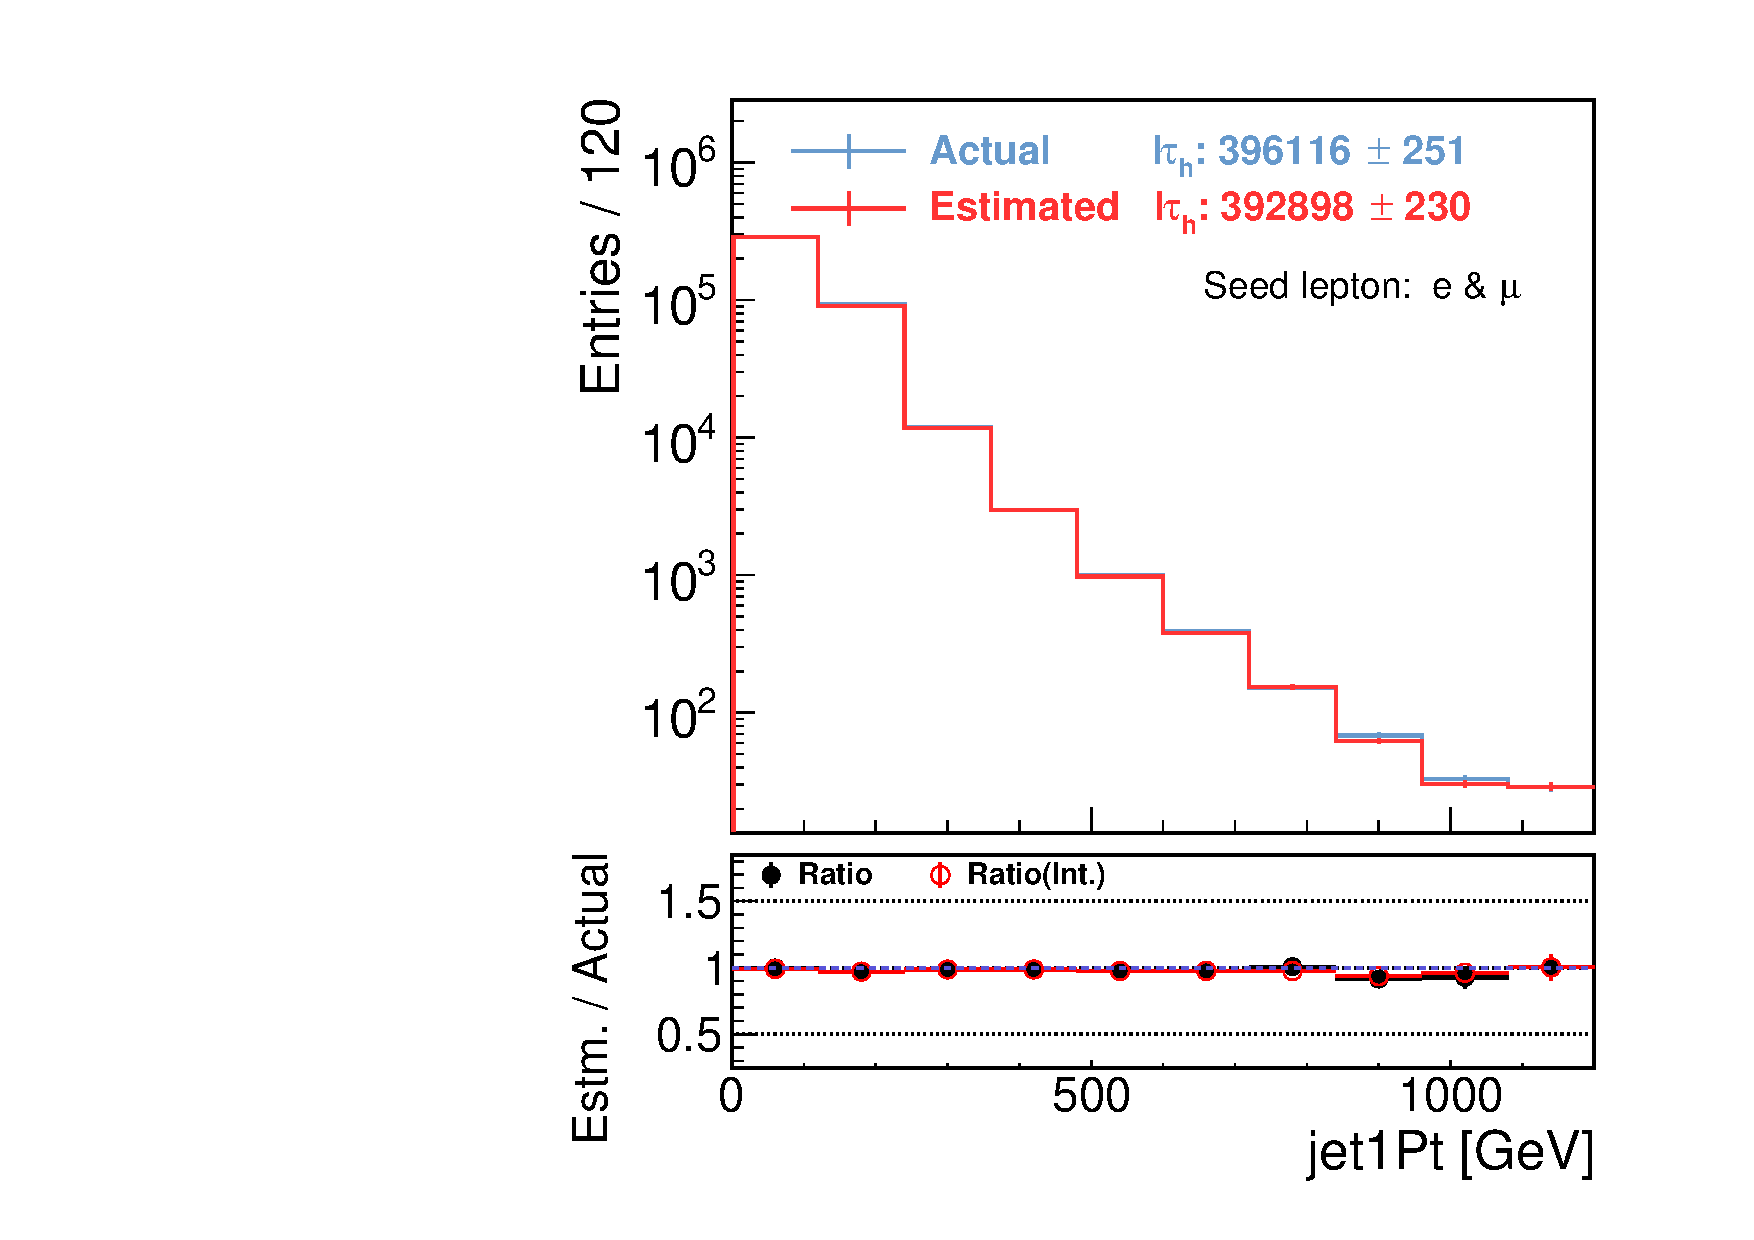
\includegraphics[width=0.32\textwidth]{figures/BGestimation/ObjReplacement/mcClosure/TauRep_emu/TauRep_emu_jet1Pt__trMode4_NoSys.pdf}}
    \subfigure[]{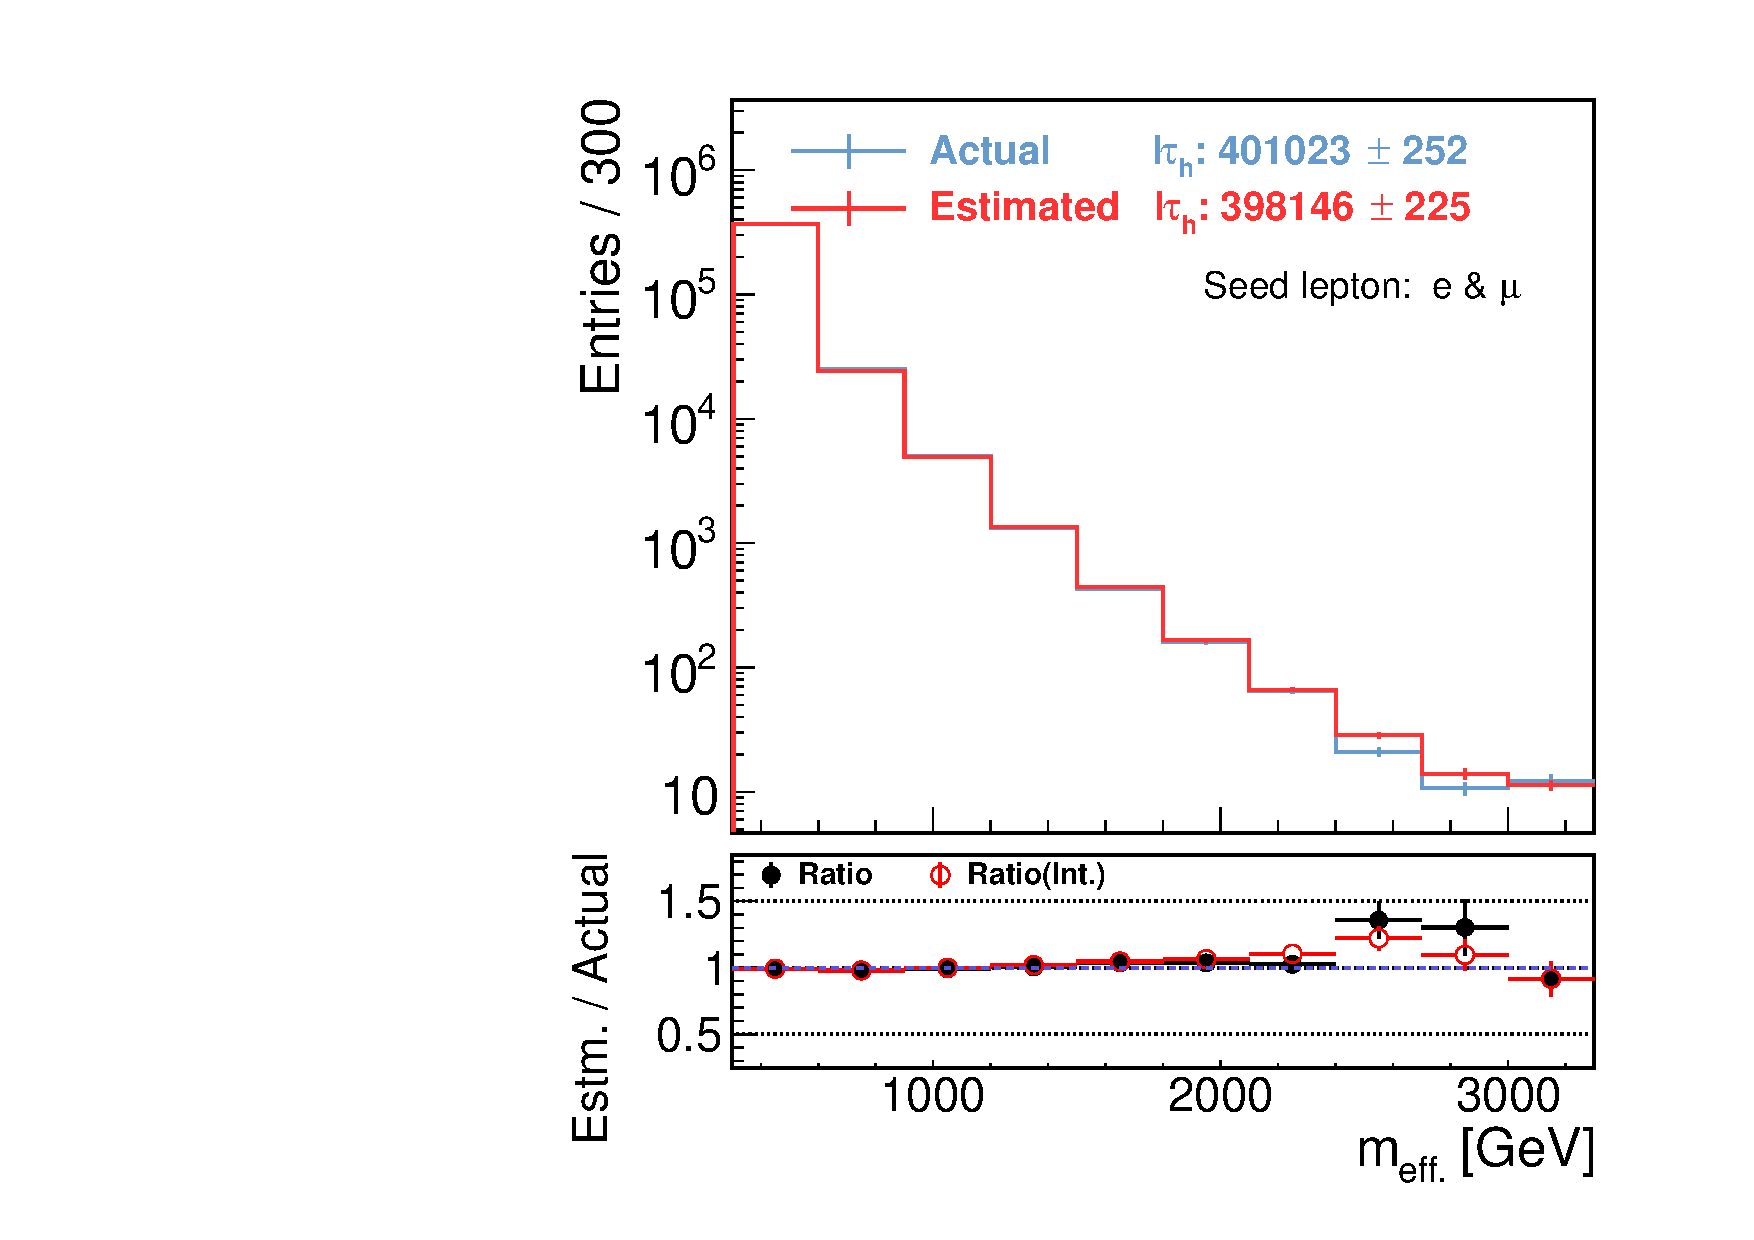
\includegraphics[width=0.32\textwidth]{figures/BGestimation/ObjReplacement/mcClosure/TauRep_emu/TauRep_emu_meffInc30__trMode4_NoSys.pdf}}
    \subfigure[]{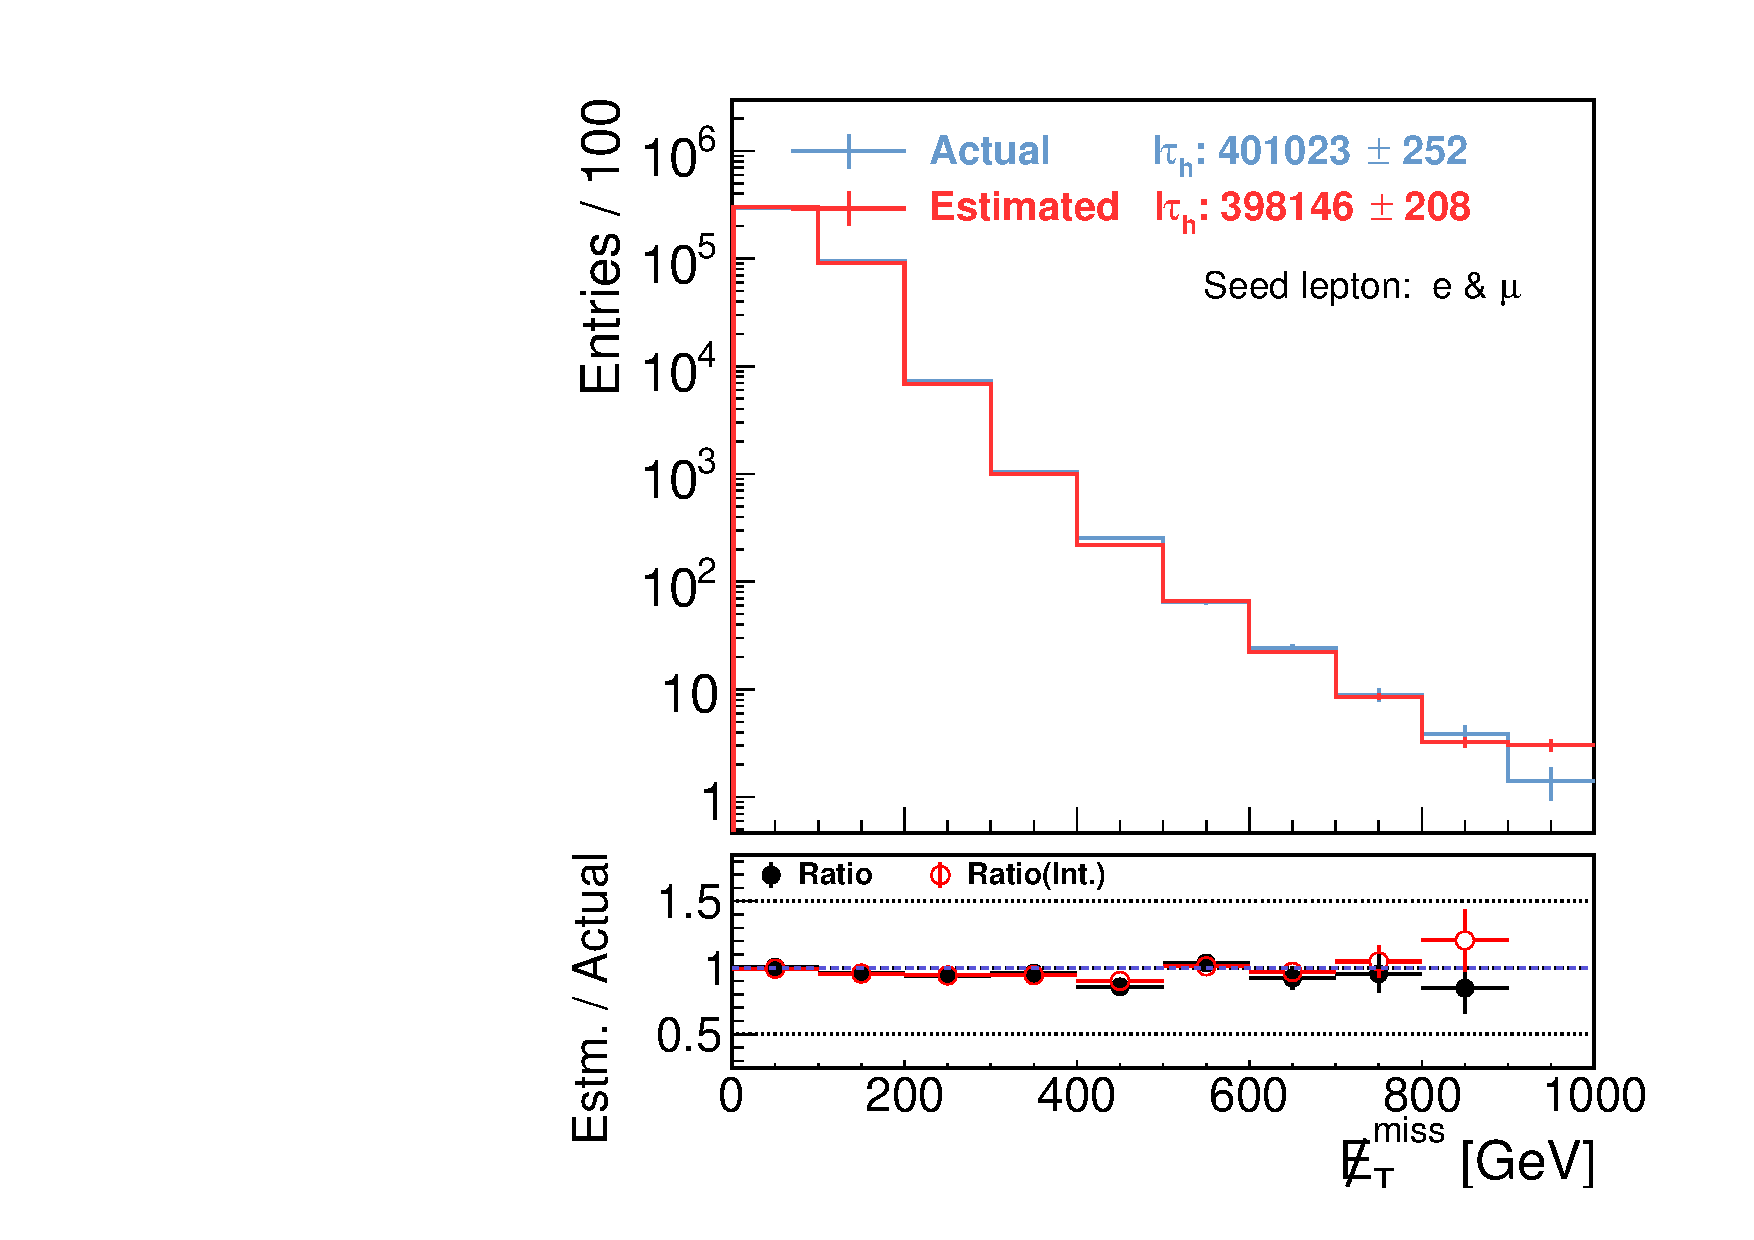
\includegraphics[width=0.32\textwidth]{figures/BGestimation/ObjReplacement/mcClosure/TauRep_emu/TauRep_emu_met__trMode4_NoSys.pdf}}
    \subfigure[]{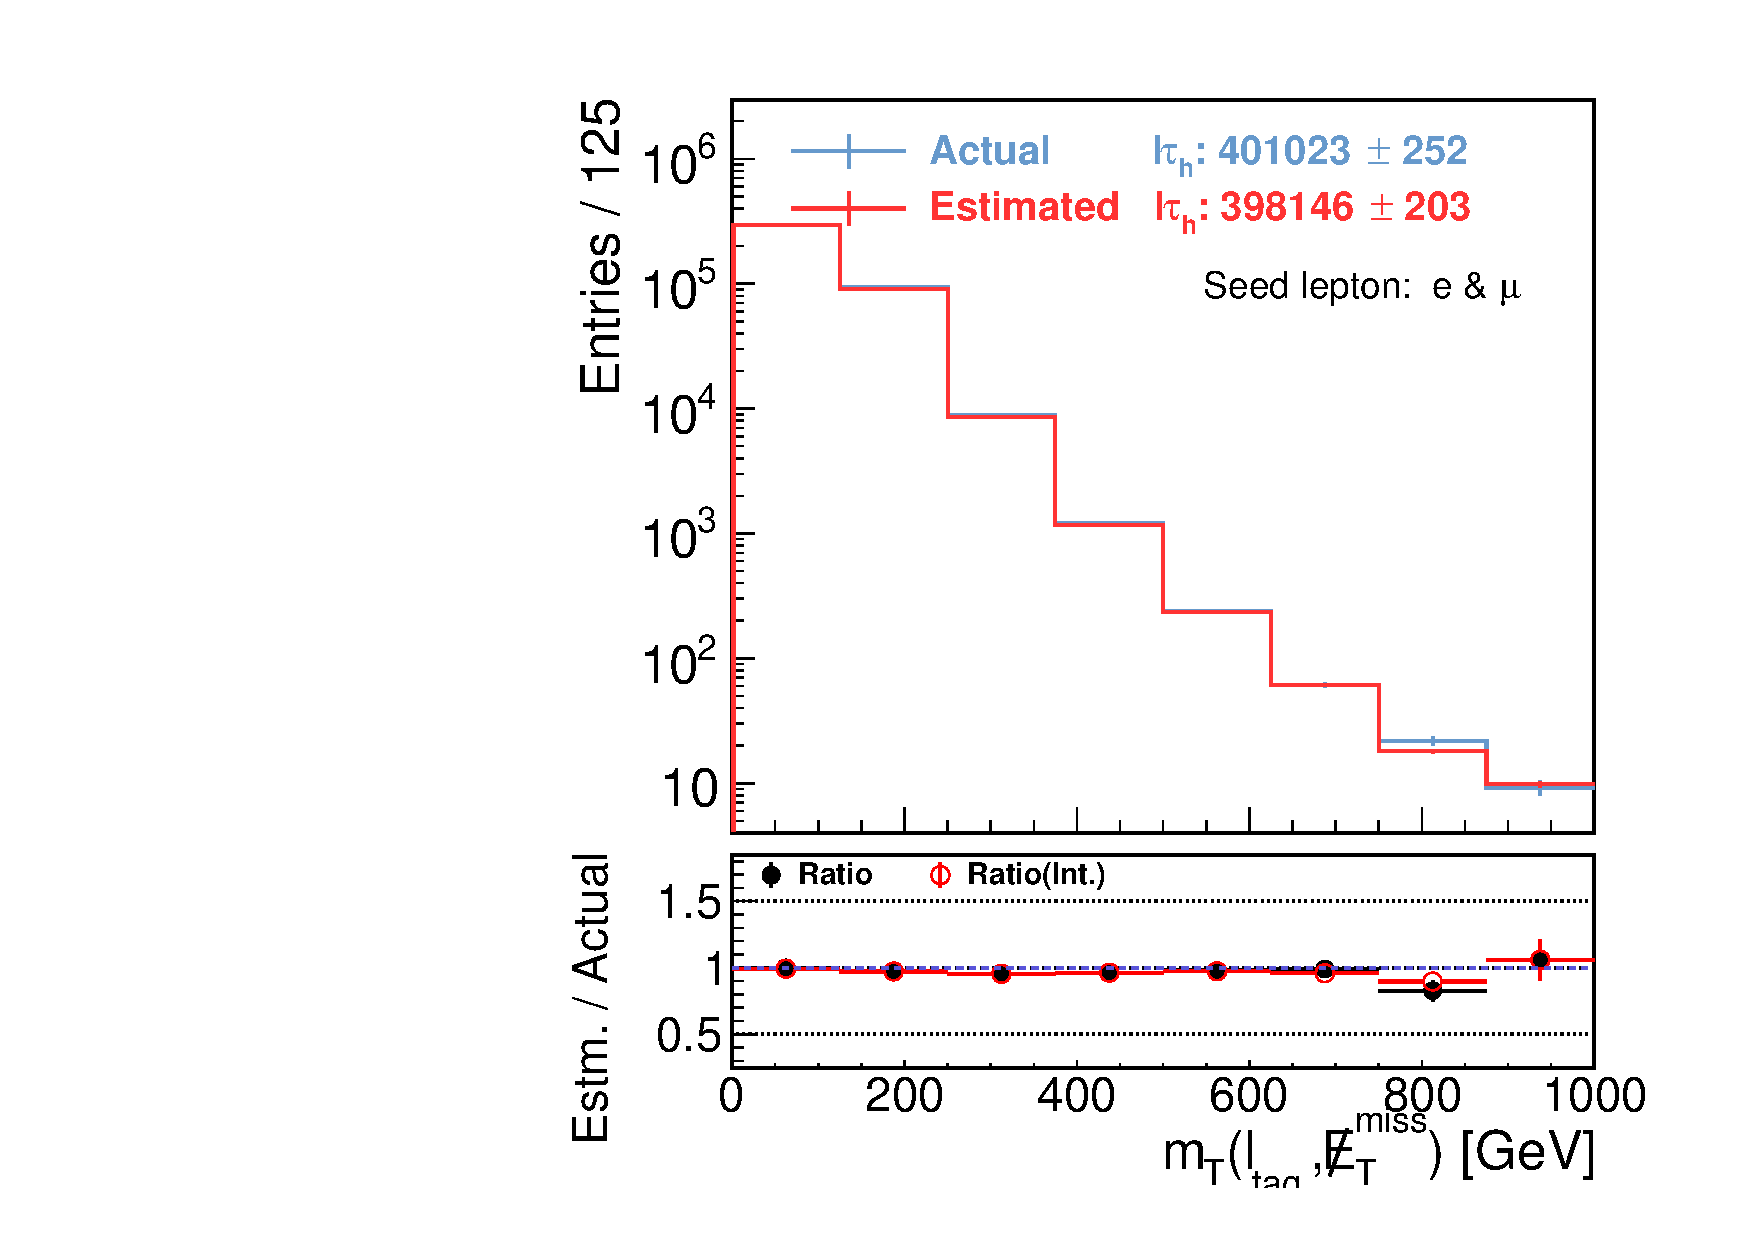
\includegraphics[width=0.32\textwidth]{figures/BGestimation/ObjReplacement/mcClosure/TauRep_emu/TauRep_emu_mt__trMode4_NoSys.pdf}}
    \subfigure[]{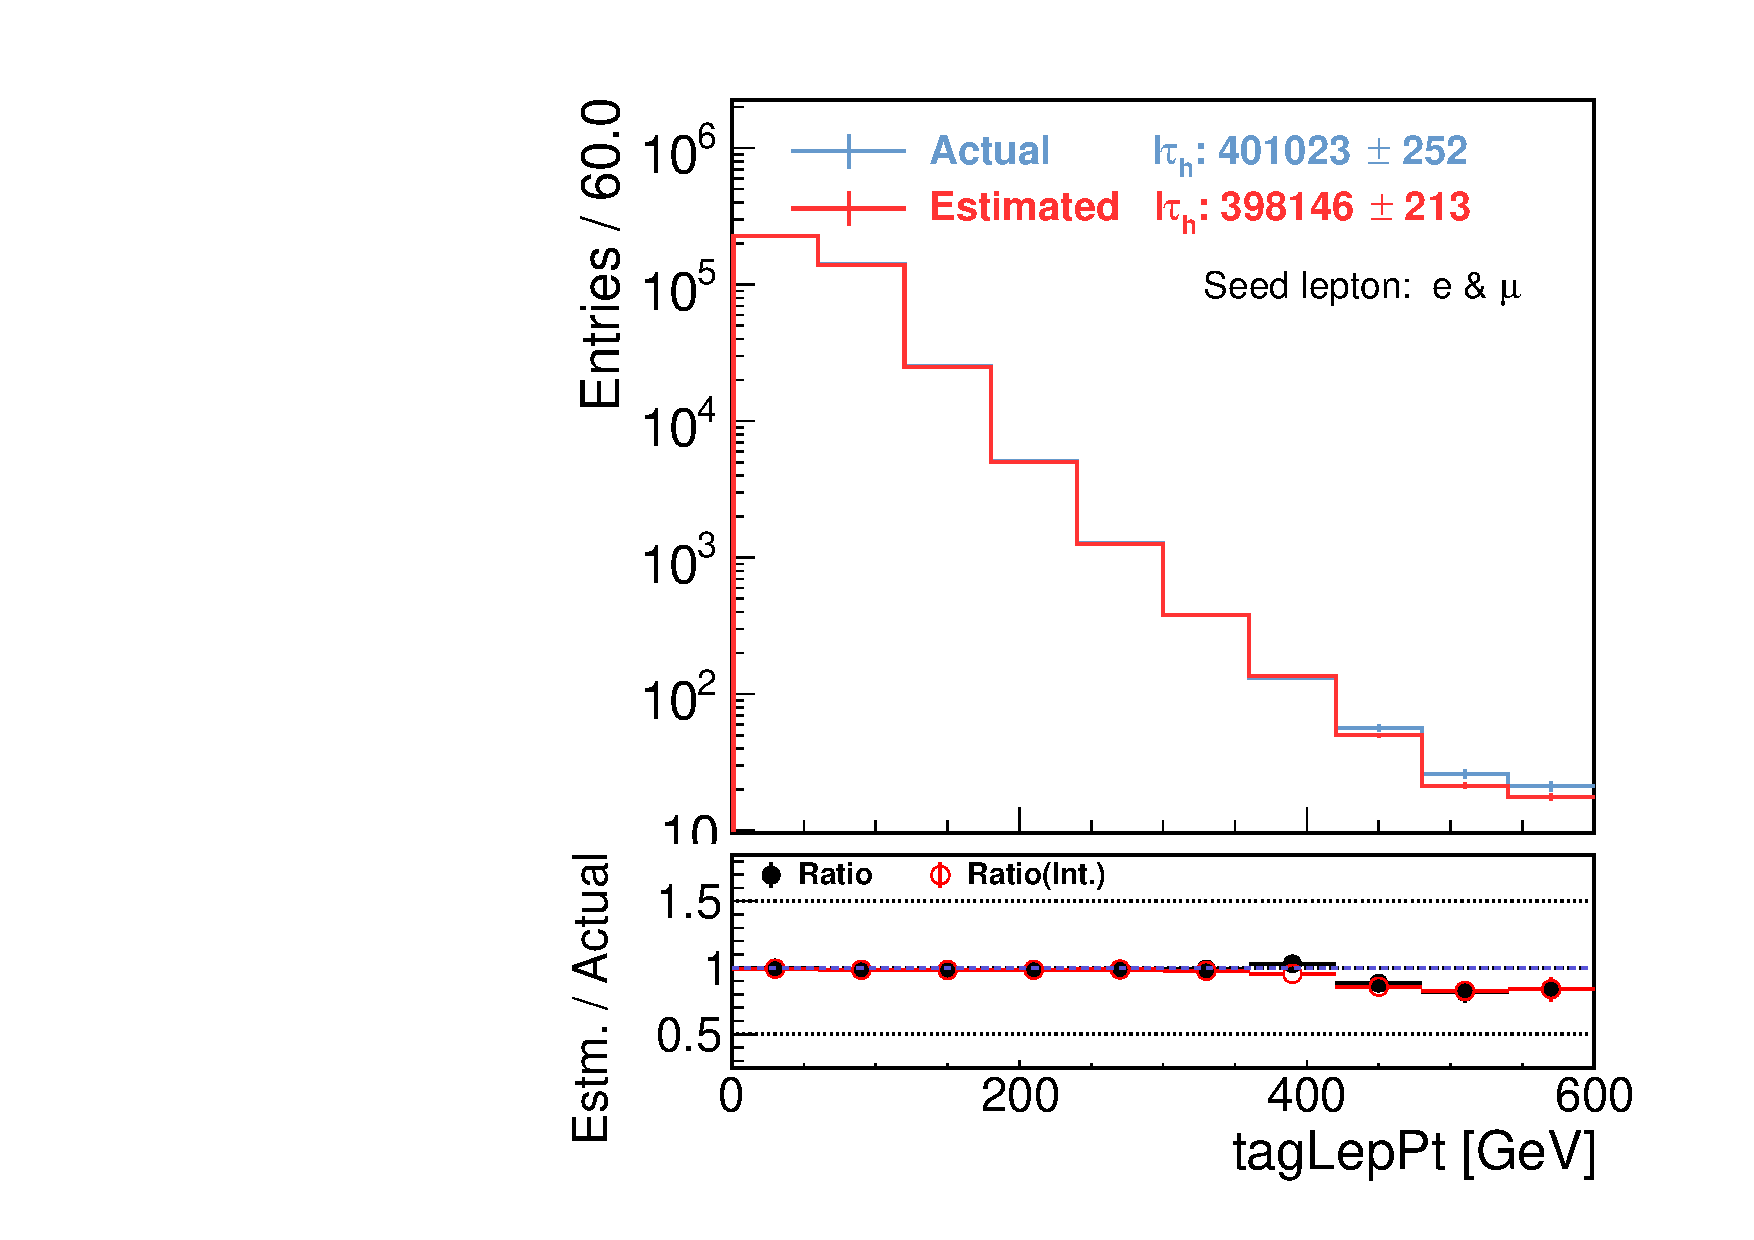
\includegraphics[width=0.32\textwidth]{figures/BGestimation/ObjReplacement/mcClosure/TauRep_emu/TauRep_emu_tagLepPt__trMode4_NoSys.pdf}}
    \subfigure[]{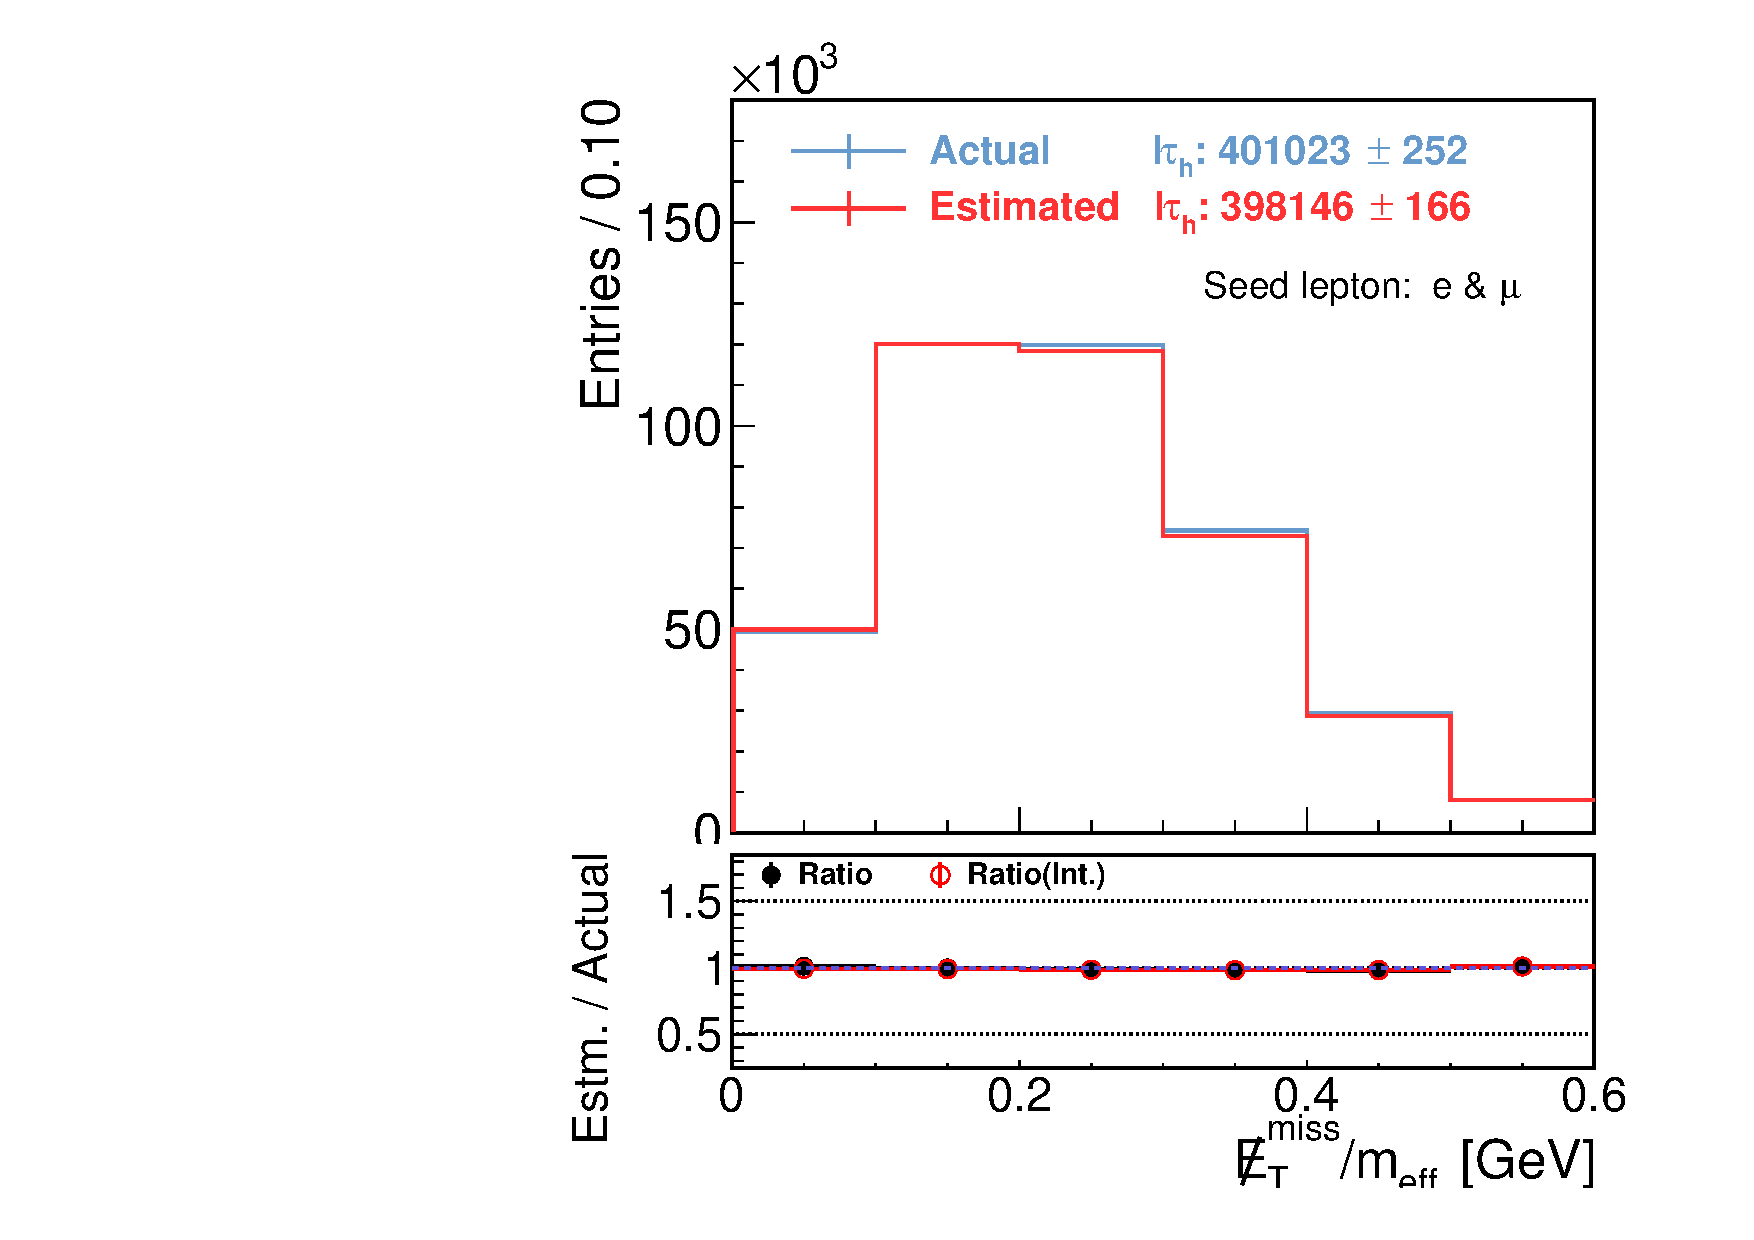
\includegraphics[width=0.32\textwidth]{figures/BGestimation/ObjReplacement/mcClosure/TauRep_emu/TauRep_emu_metOverMeff__trMode4_NoSys.pdf}}
    \subfigure[]{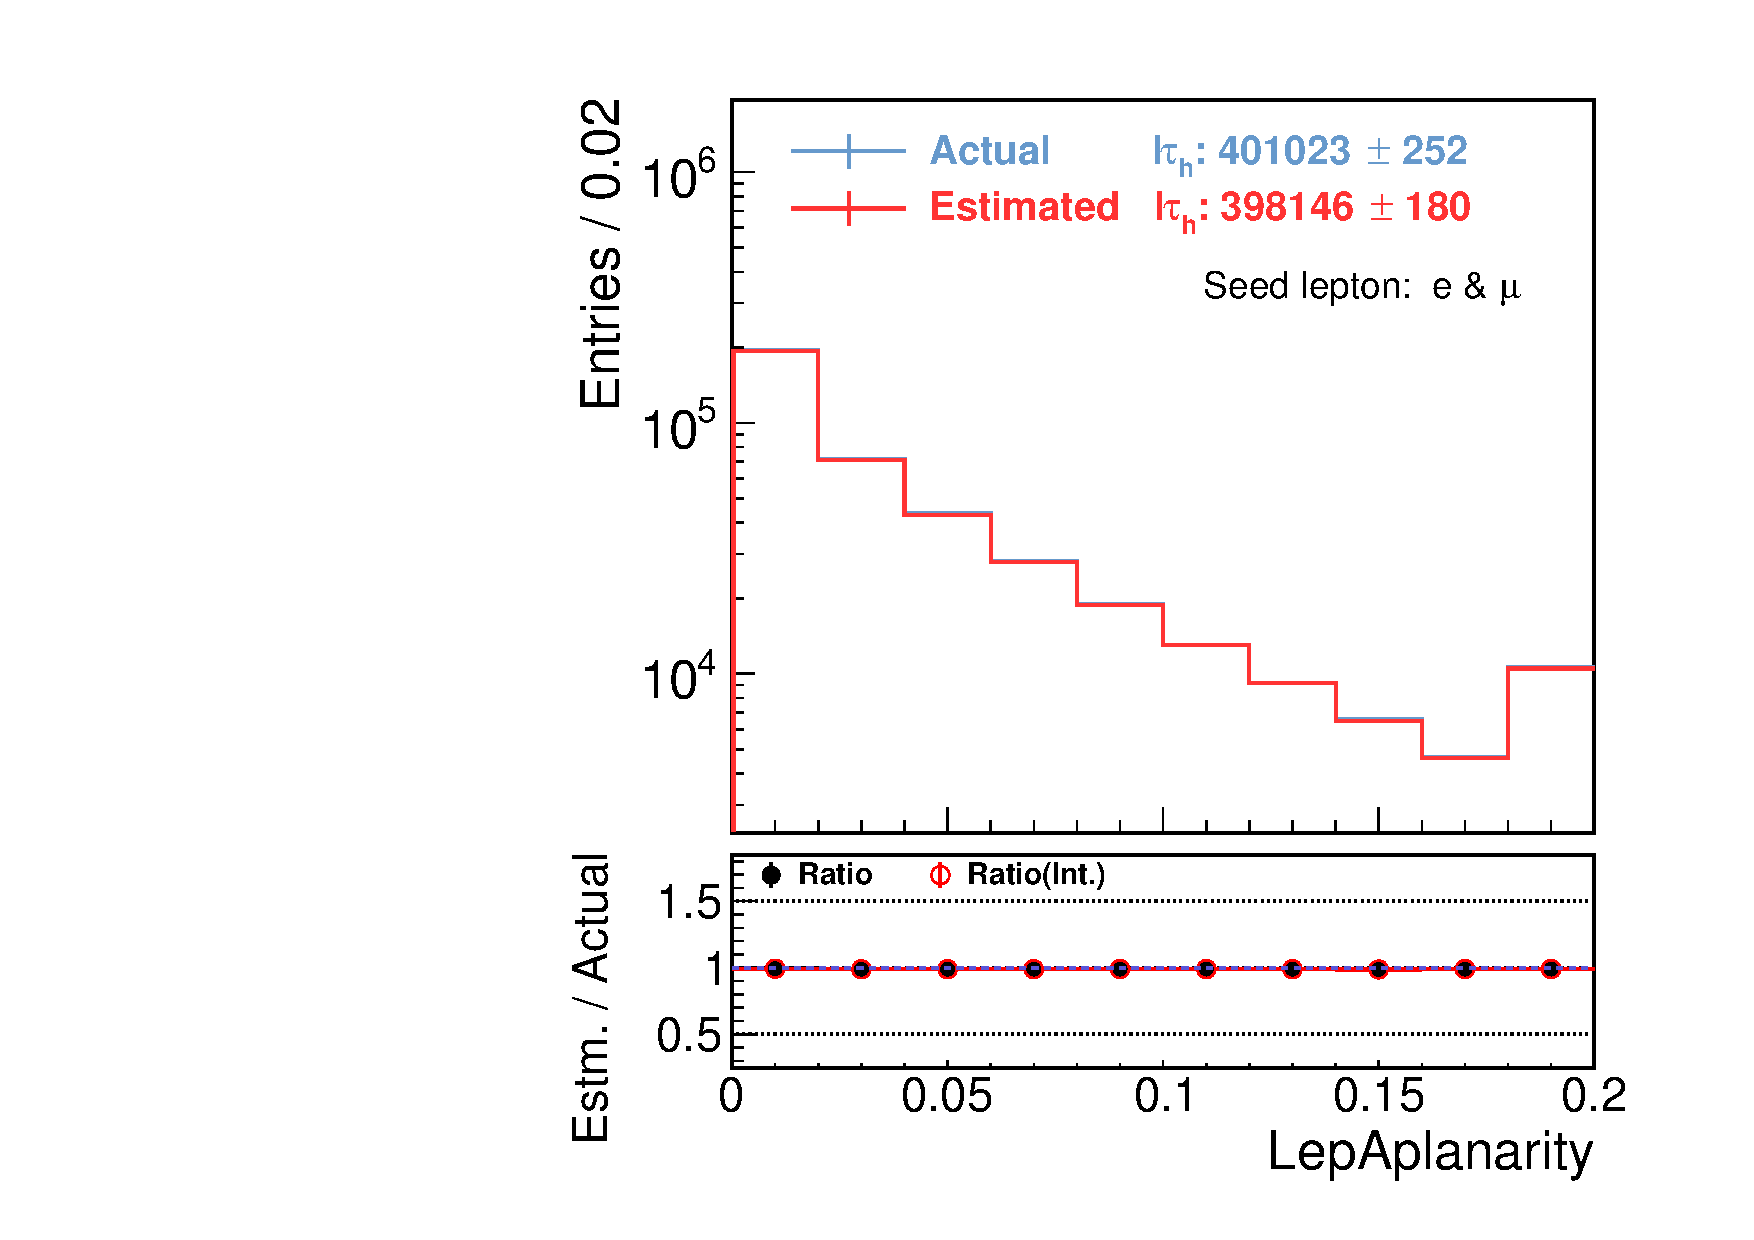
\includegraphics[width=0.32\textwidth]{figures/BGestimation/ObjReplacement/mcClosure/TauRep_emu/TauRep_emu_LepAplanarity__trMode4_NoSys.pdf}}
    \subfigure[]{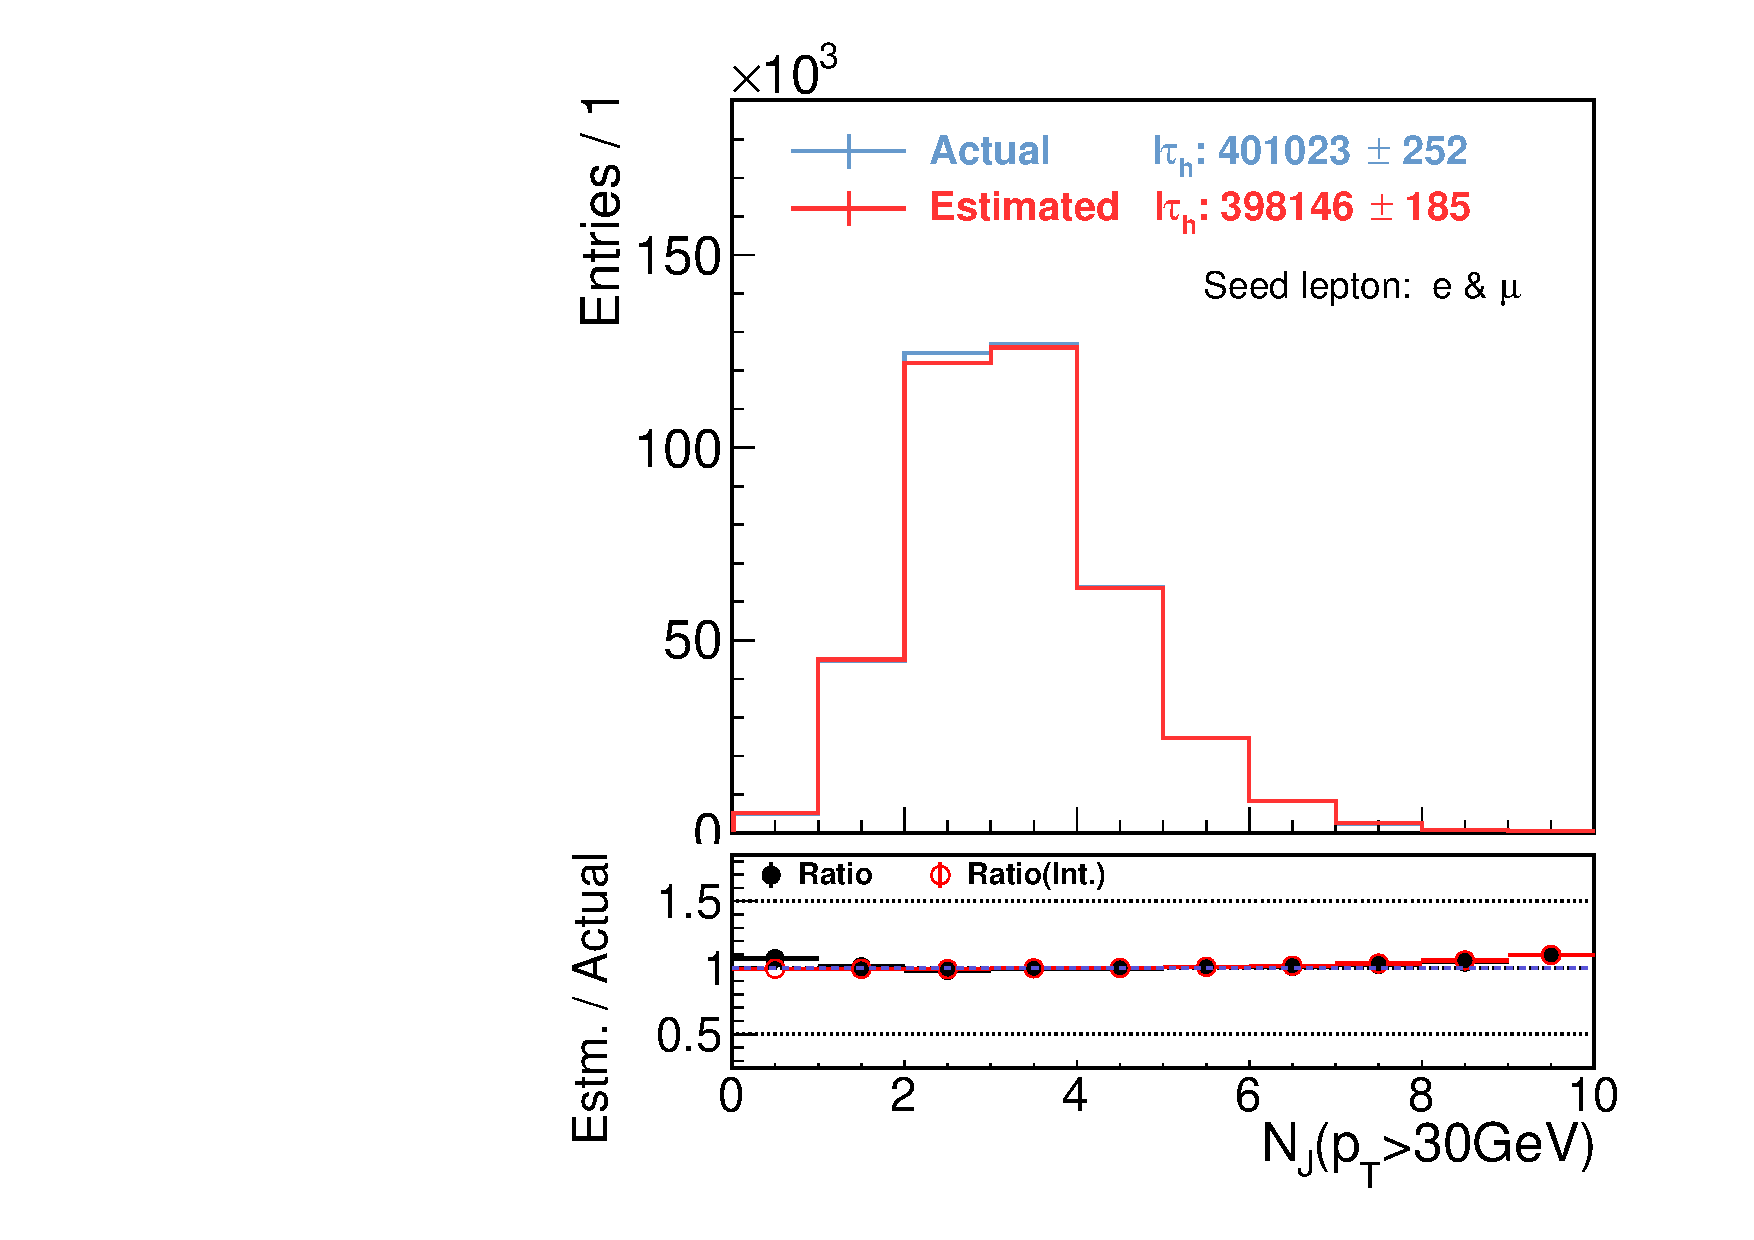
\includegraphics[width=0.32\textwidth]{figures/BGestimation/ObjReplacement/mcClosure/TauRep_emu/TauRep_emu_nJet30__trMode4_NoSys.pdf}}
    \subfigure[]{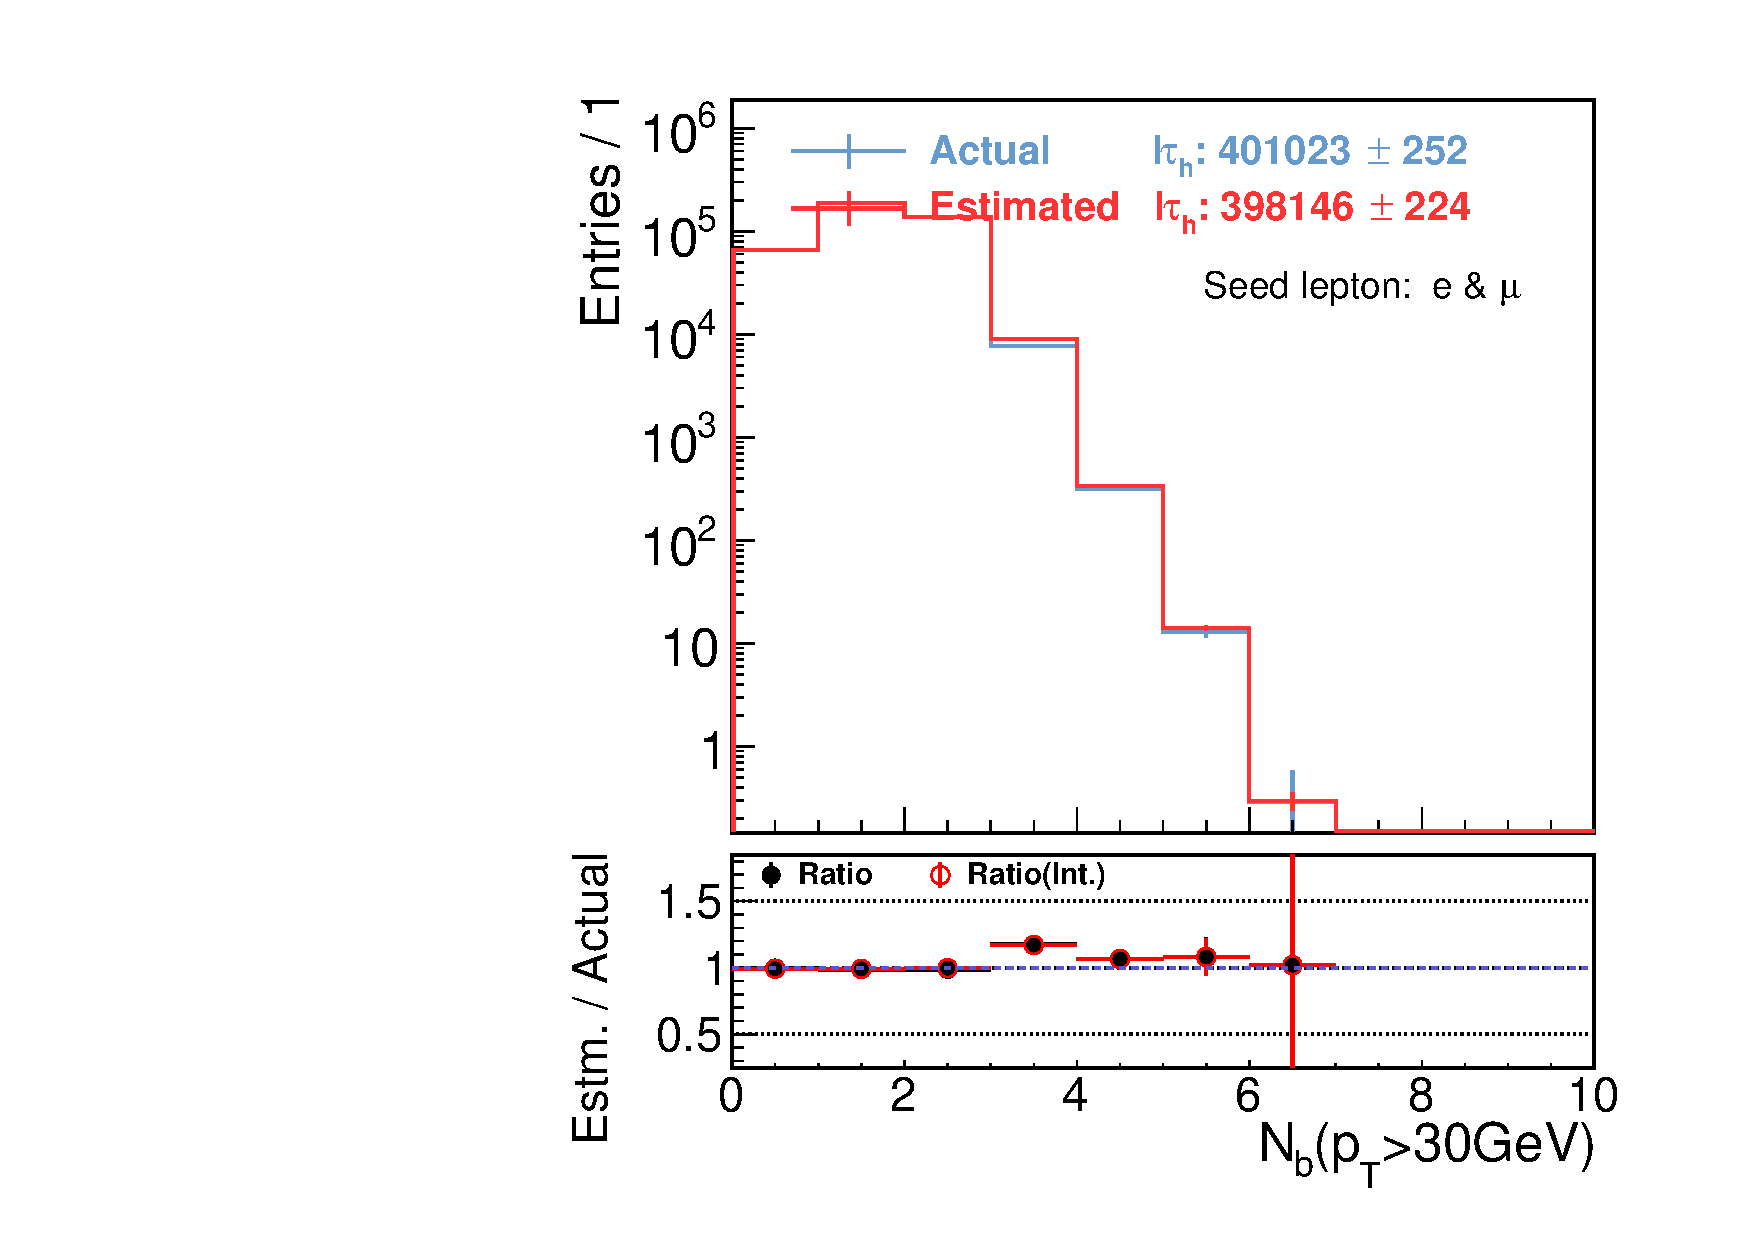
\includegraphics[width=0.32\textwidth]{figures/BGestimation/ObjReplacement/mcClosure/TauRep_emu/TauRep_emu_nBJet30__trMode4_NoSys.pdf}}
    \caption{ MC closure test for \textbf{tau replacement} using $t\bar{t}$ MC sample. Seed events are collected by the single-lepton trigger. $p_T>35\gev$ for the leading lepton is required. \textbf{Both electrons and muons in the seed events are replaced}. Red points in the bottom plots show the ratio of integrated yields for the two histograms above the x-position that the point indicates. \label{fig::ObjReplace::mcClosure_TauRep_emu} }
\end{figure}
 %%%%%%%%%%%%%%%%%%%%%%%%%%


% ---------- mcClosure::plot::softLep
%%%%% METHNAME %%%%%%%%%%%%%%%%%%%%%%%%%%
\begin{figure}[h]
  \centering
    \subfig{0.28}{figures/BGestimation/ObjReplacement/mcClosure_softlep/MisLep_el_softLep/MisLep_el_jet1Pt__trMode4_NoSys_softLep.pdf}{$\pt$ of the leading jet}
    \subfig{0.28}{figures/BGestimation/ObjReplacement/mcClosure_softlep/MisLep_el_softLep/MisLep_el_meffInc30__trMode4_NoSys_softLep.pdf}{$\meffInc$}
    \subfig{0.28}{figures/BGestimation/ObjReplacement/mcClosure_softlep/MisLep_el_softLep/MisLep_el_met__trMode4_NoSys_softLep.pdf}{$\met$}
    \subfig{0.28}{figures/BGestimation/ObjReplacement/mcClosure_softlep/MisLep_el_softLep/MisLep_el_mt__trMode4_NoSys_softLep.pdf}{$\mt$}
    \subfig{0.28}{figures/BGestimation/ObjReplacement/mcClosure_softlep/MisLep_el_softLep/MisLep_el_metOverMeff__trMode4_NoSys_softLep.pdf}{$\met/\meffInc$}
    \subfig{0.28}{figures/BGestimation/ObjReplacement/mcClosure_softlep/MisLep_el_softLep/MisLep_el_LepAplanarity__trMode4_NoSys_softLep.pdf}{Aplanarity}
    \subfig{0.28}{figures/BGestimation/ObjReplacement/mcClosure_softlep/MisLep_el_softLep/MisLep_el_min_dPhi_4j__trMode4_NoSys_softLep.pdf}{$\mindPhiFourJet$}
    \subfig{0.28}{figures/BGestimation/ObjReplacement/mcClosure_softlep/MisLep_el_softLep/MisLep_el_nJet30__trMode4_NoSys_softLep.pdf}{Jet multiplicity}
    \subfig{0.28}{figures/BGestimation/ObjReplacement/mcClosure_softlep/MisLep_el_softLep/MisLep_el_nBJet30__trMode4_NoSys_softLep.pdf}{$b$-jet multiplicity}
    \caption{ MC closure test for \textbf{missing lepton replacement} using $t\bar{t}$ MC sample. Seed events are collected by the use of MET trigger. $p_T<35\gev$ for the leading lepton is required. \textbf{Only electrons in the seed events are replaced}. Red points in the bottom plots show the ratio of integrated yields for the two histograms above the x-position that the point indicates. \label{fig::ObjReplace::mcClosure_softLep_MisLep_el} }
\end{figure}
 %%%%%%%%%%%%%%%%%%%%%%%%%%

%%%%% METHNAME %%%%%%%%%%%%%%%%%%%%%%%%%%
\begin{figure}[h]
  \centering
    \subfigure[]{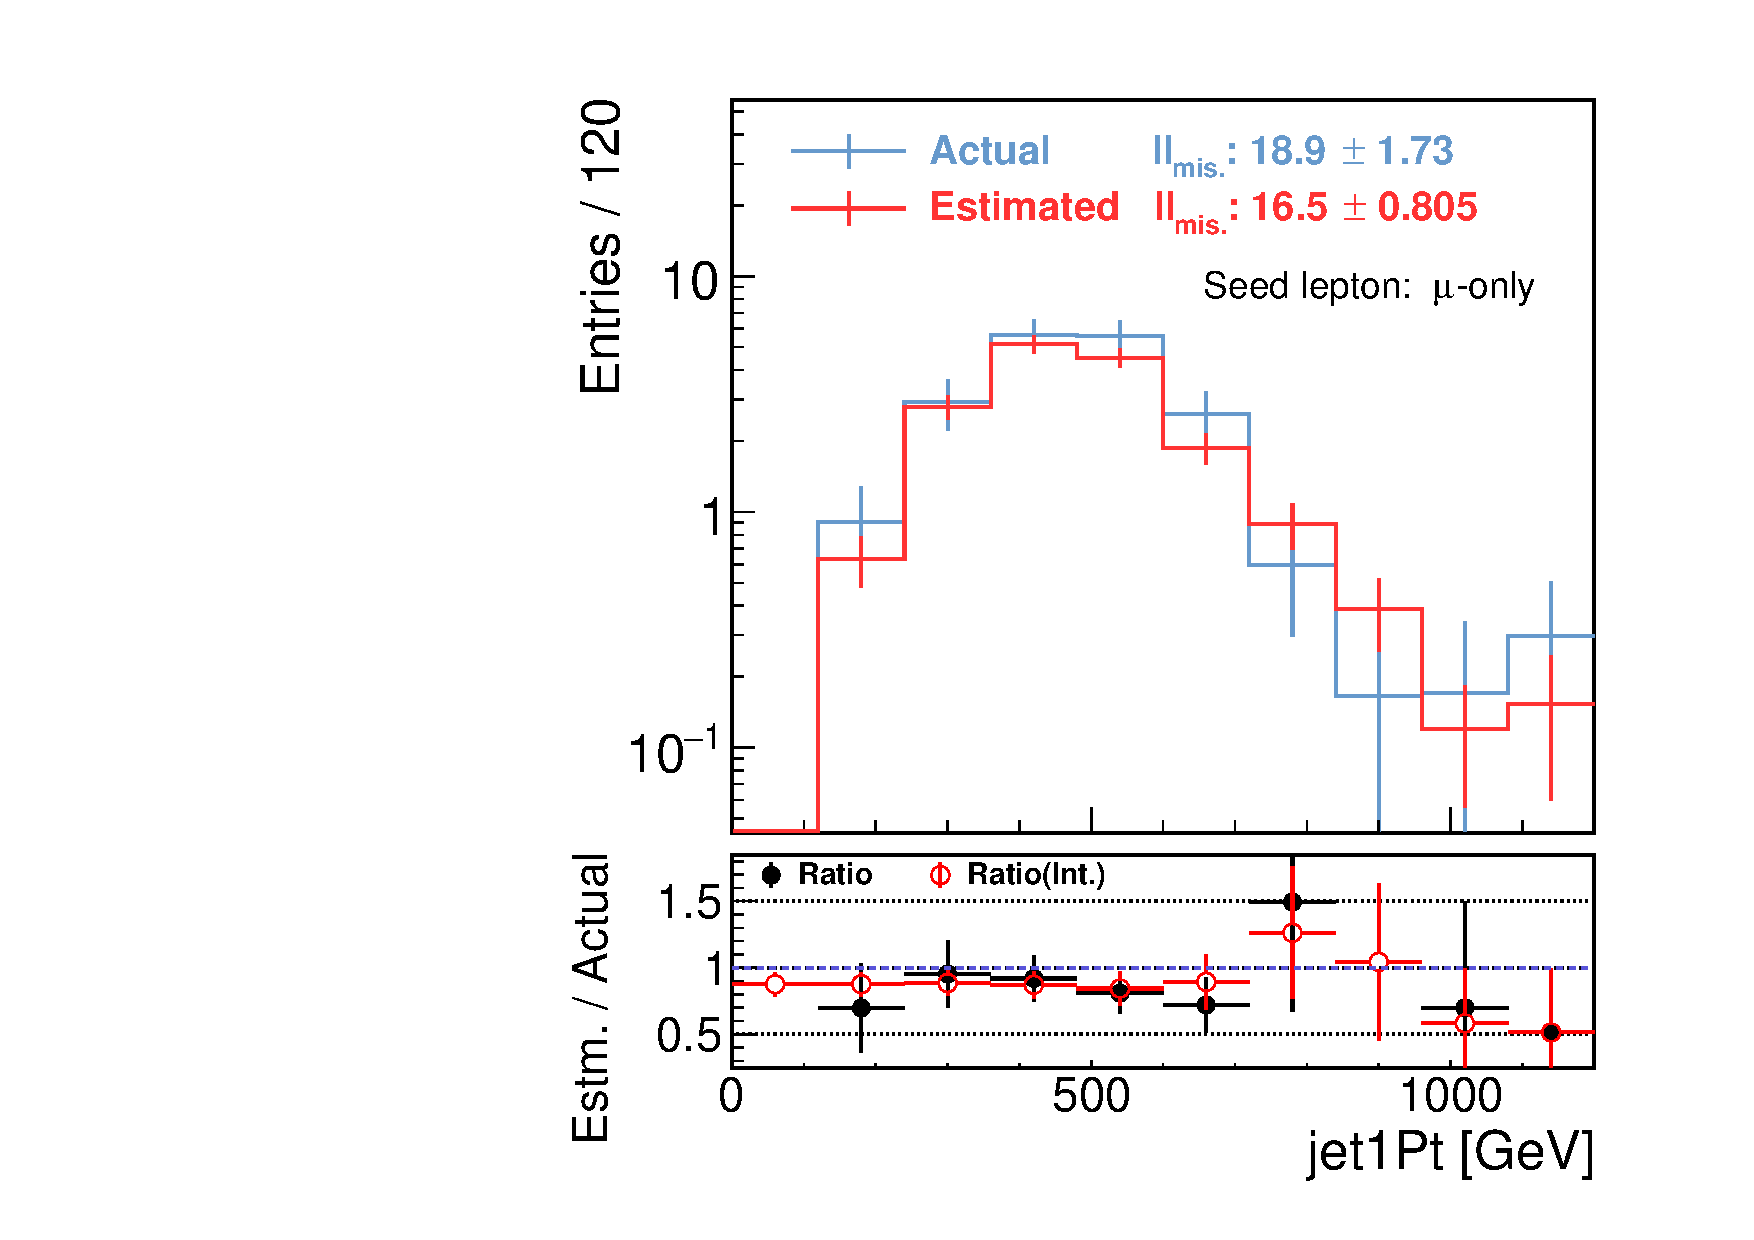
\includegraphics[width=0.32\textwidth]{figures/BGestimation/ObjReplacement/mcClosure_softLep/MisLep_mu_softLep/MisLep_mu_jet1Pt__trMode4_NoSys_softLep.pdf}}
    \subfigure[]{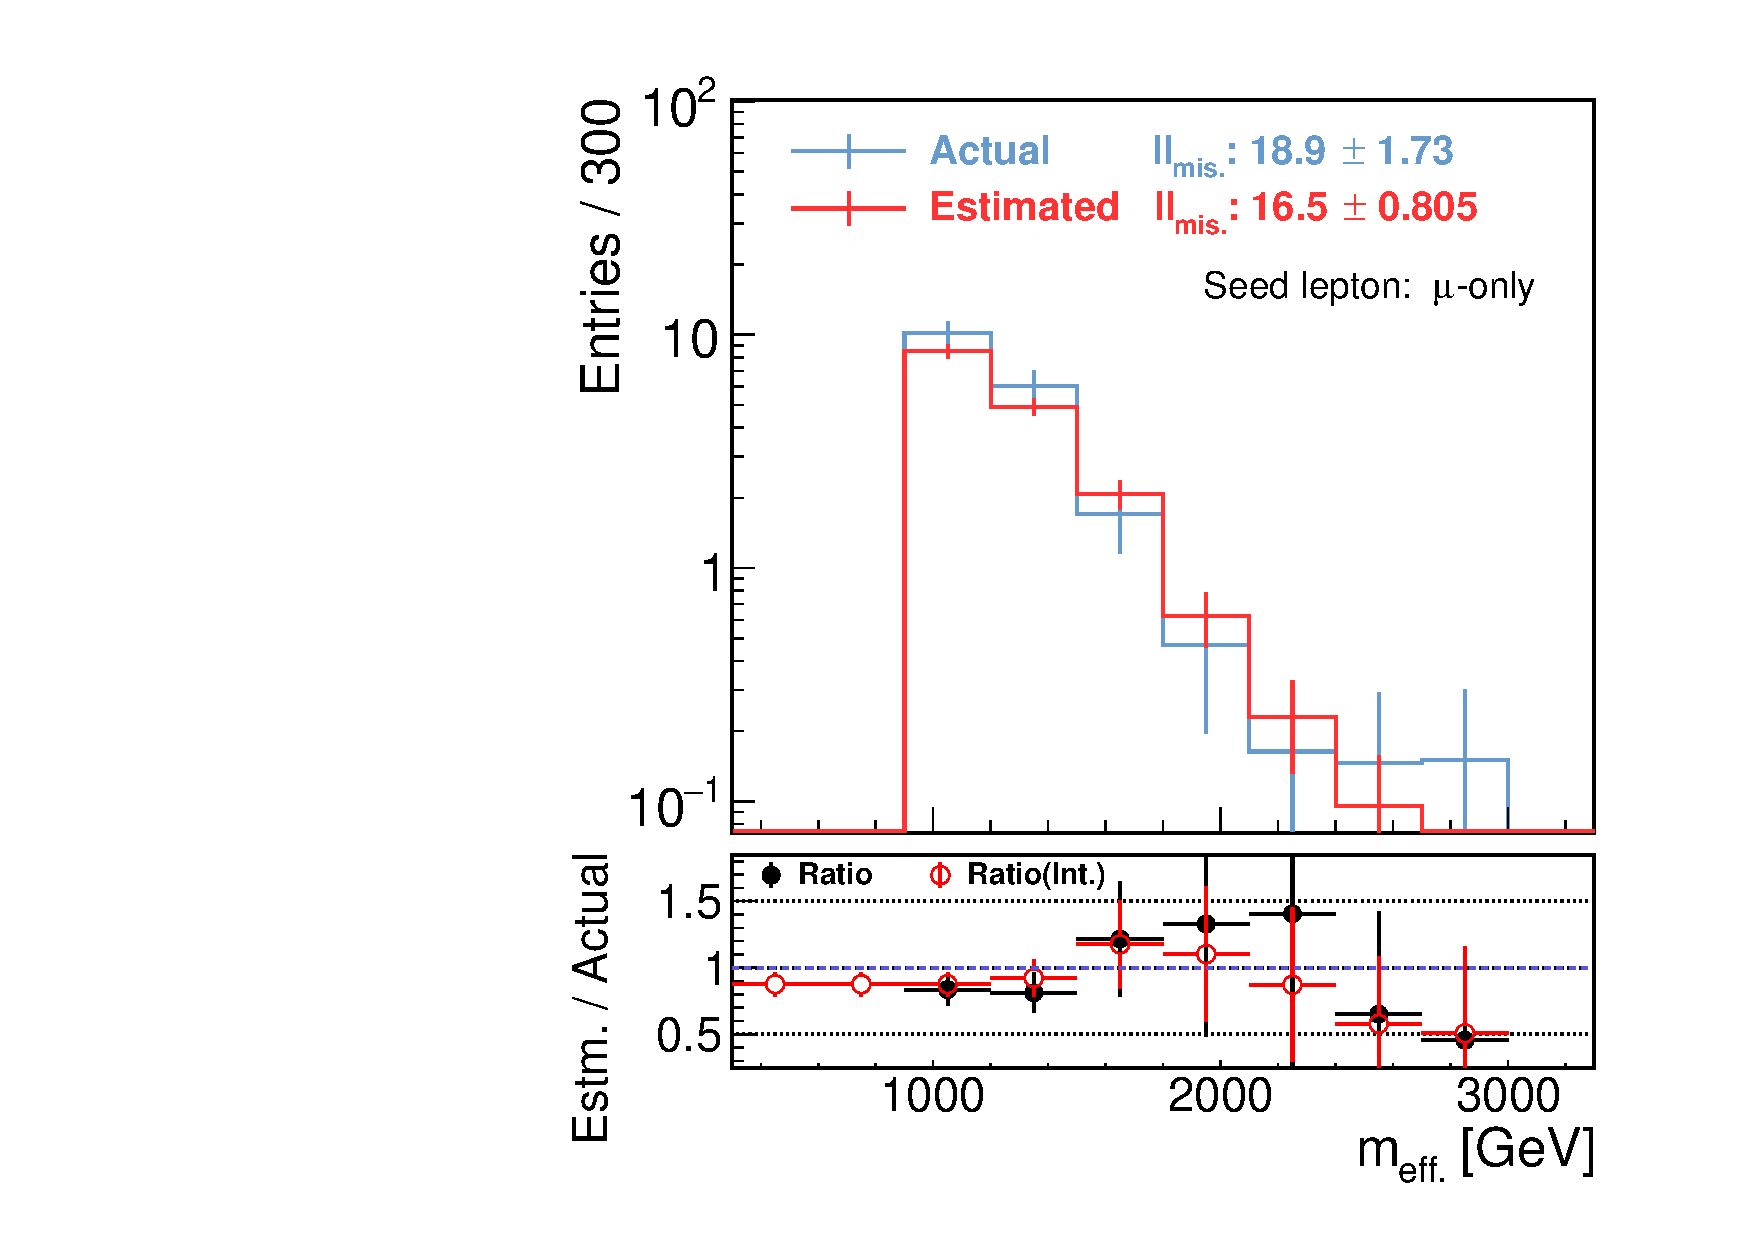
\includegraphics[width=0.32\textwidth]{figures/BGestimation/ObjReplacement/mcClosure_softLep/MisLep_mu_softLep/MisLep_mu_meffInc30__trMode4_NoSys_softLep.pdf}}
    \subfigure[]{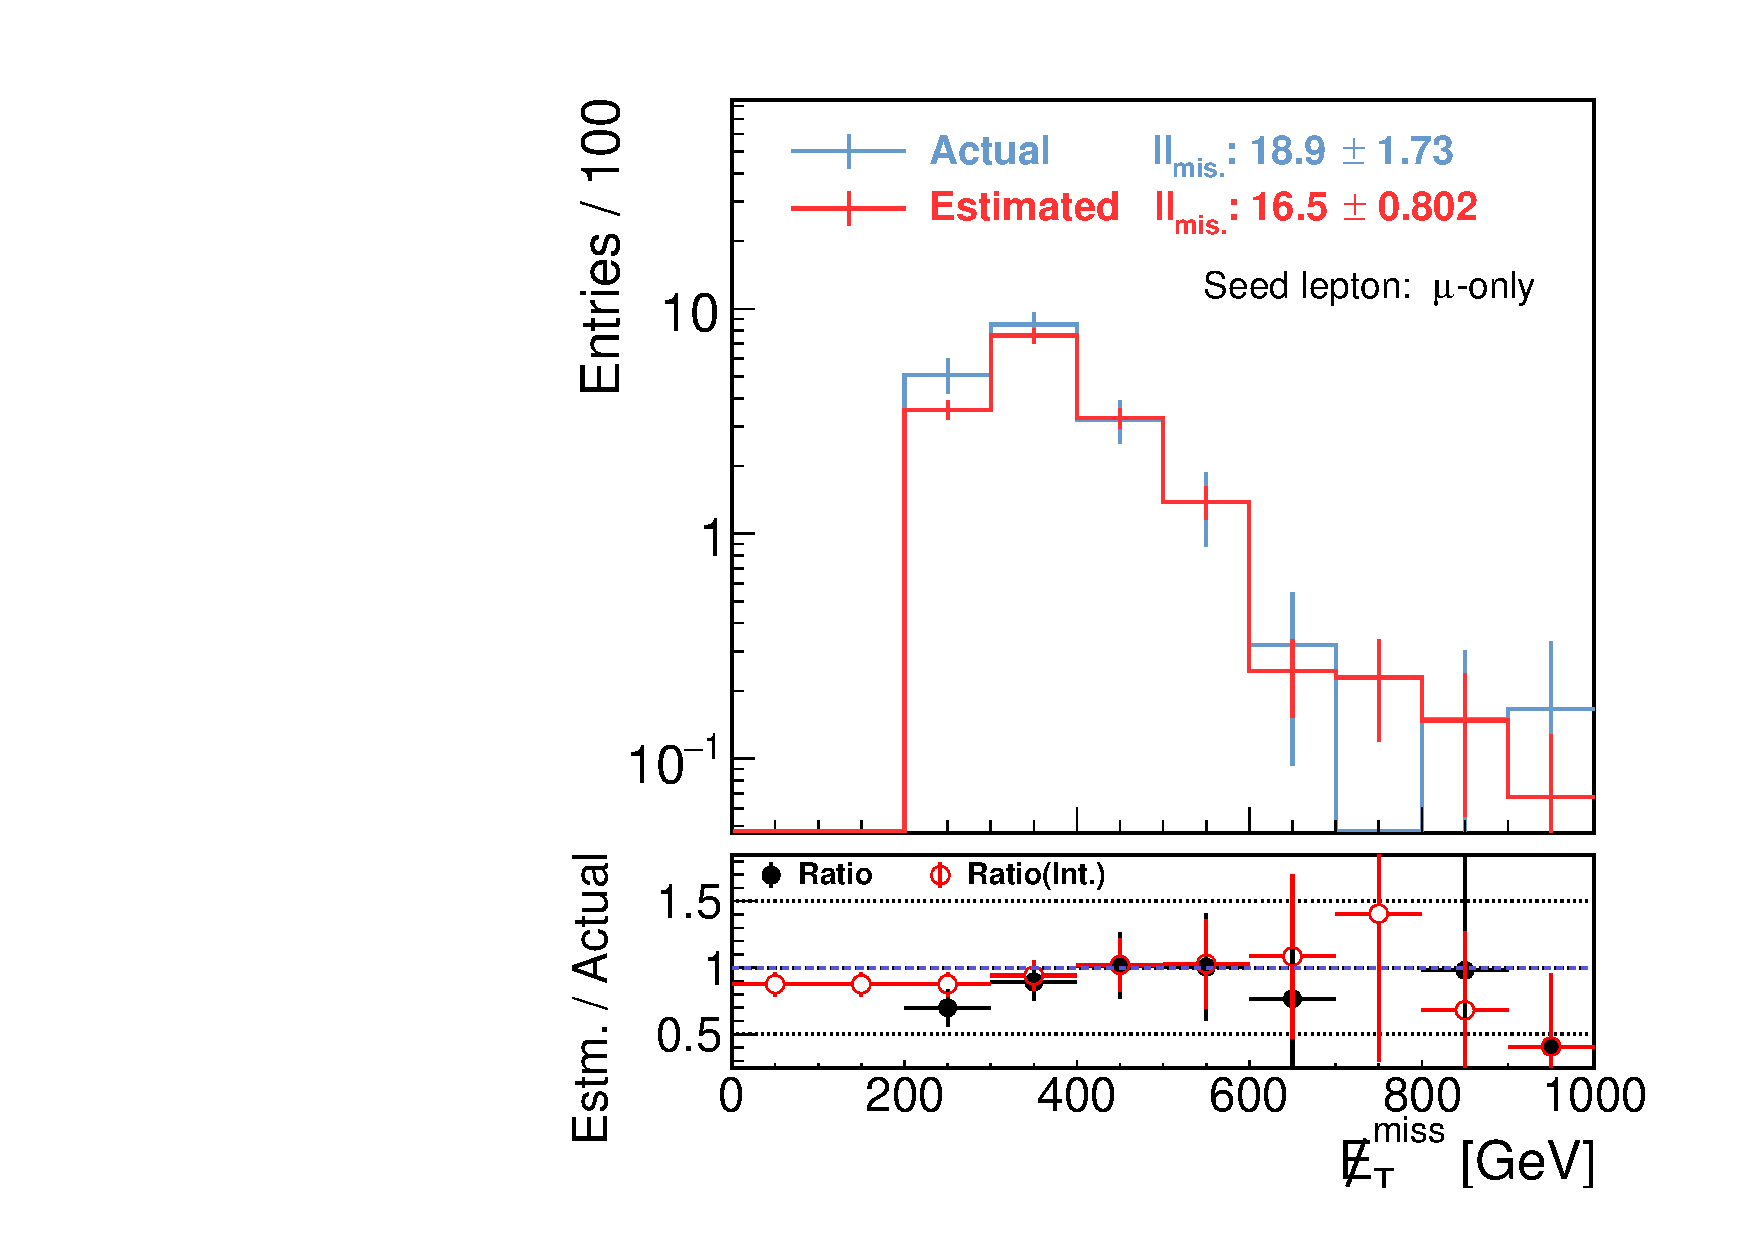
\includegraphics[width=0.32\textwidth]{figures/BGestimation/ObjReplacement/mcClosure_softLep/MisLep_mu_softLep/MisLep_mu_met__trMode4_NoSys_softLep.pdf}}
    \subfigure[]{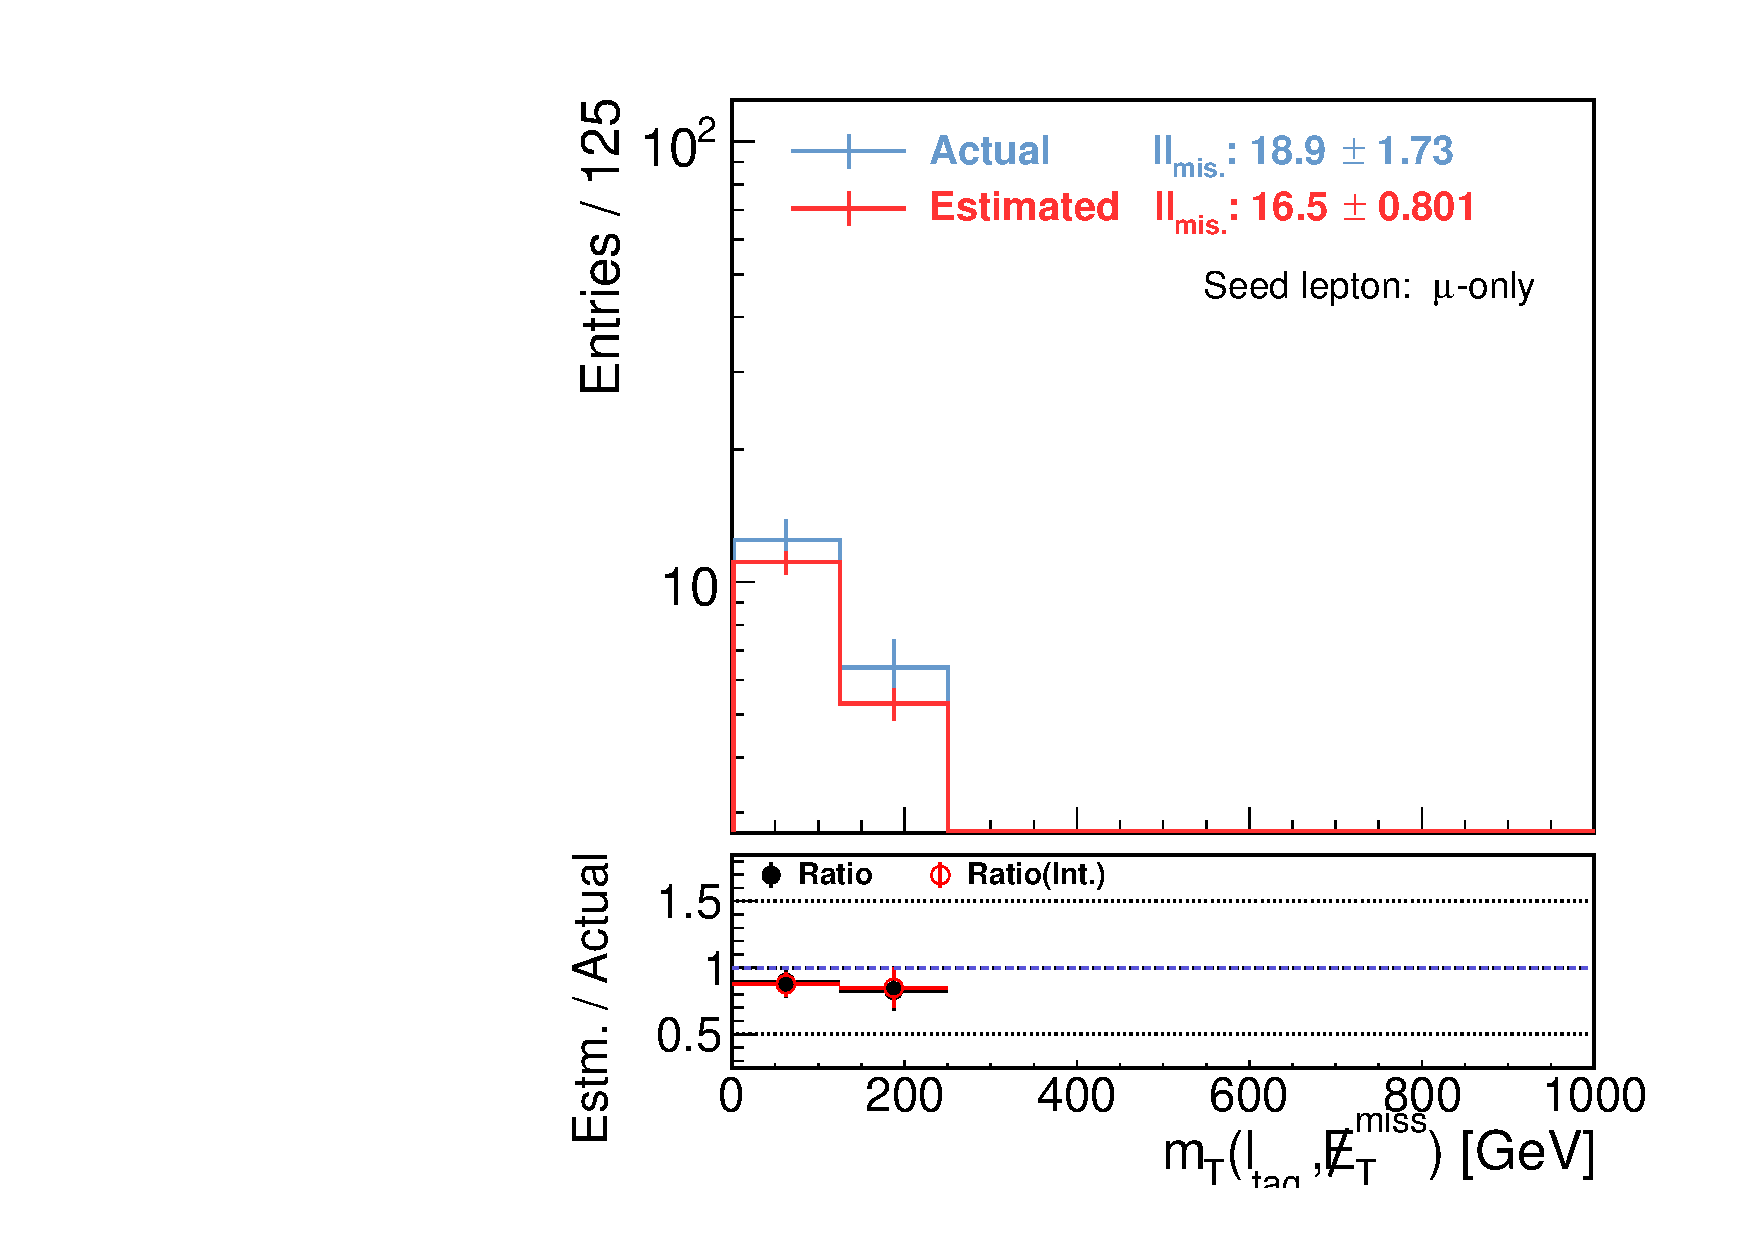
\includegraphics[width=0.32\textwidth]{figures/BGestimation/ObjReplacement/mcClosure_softLep/MisLep_mu_softLep/MisLep_mu_mt__trMode4_NoSys_softLep.pdf}}
    \subfigure[]{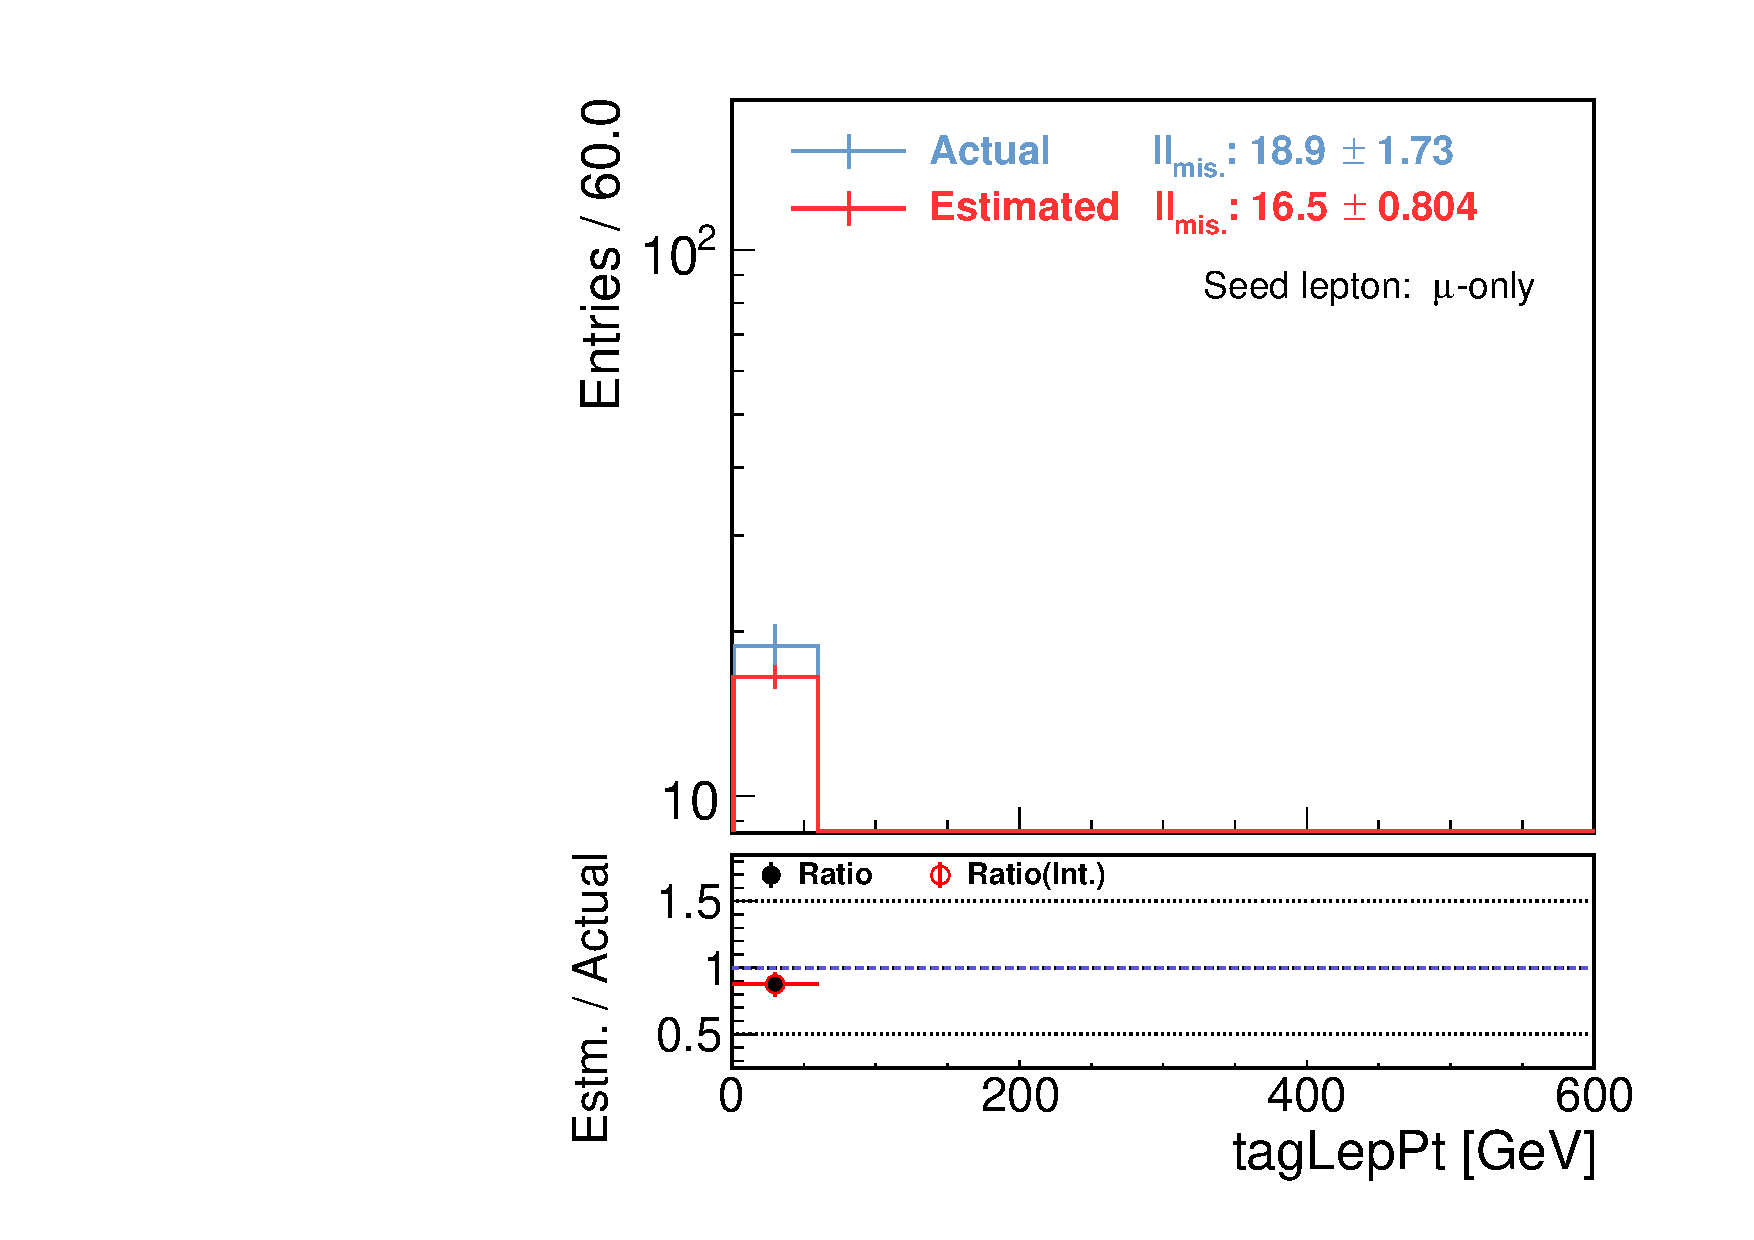
\includegraphics[width=0.32\textwidth]{figures/BGestimation/ObjReplacement/mcClosure_softLep/MisLep_mu_softLep/MisLep_mu_tagLepPt__trMode4_NoSys_softLep.pdf}}
    \subfigure[]{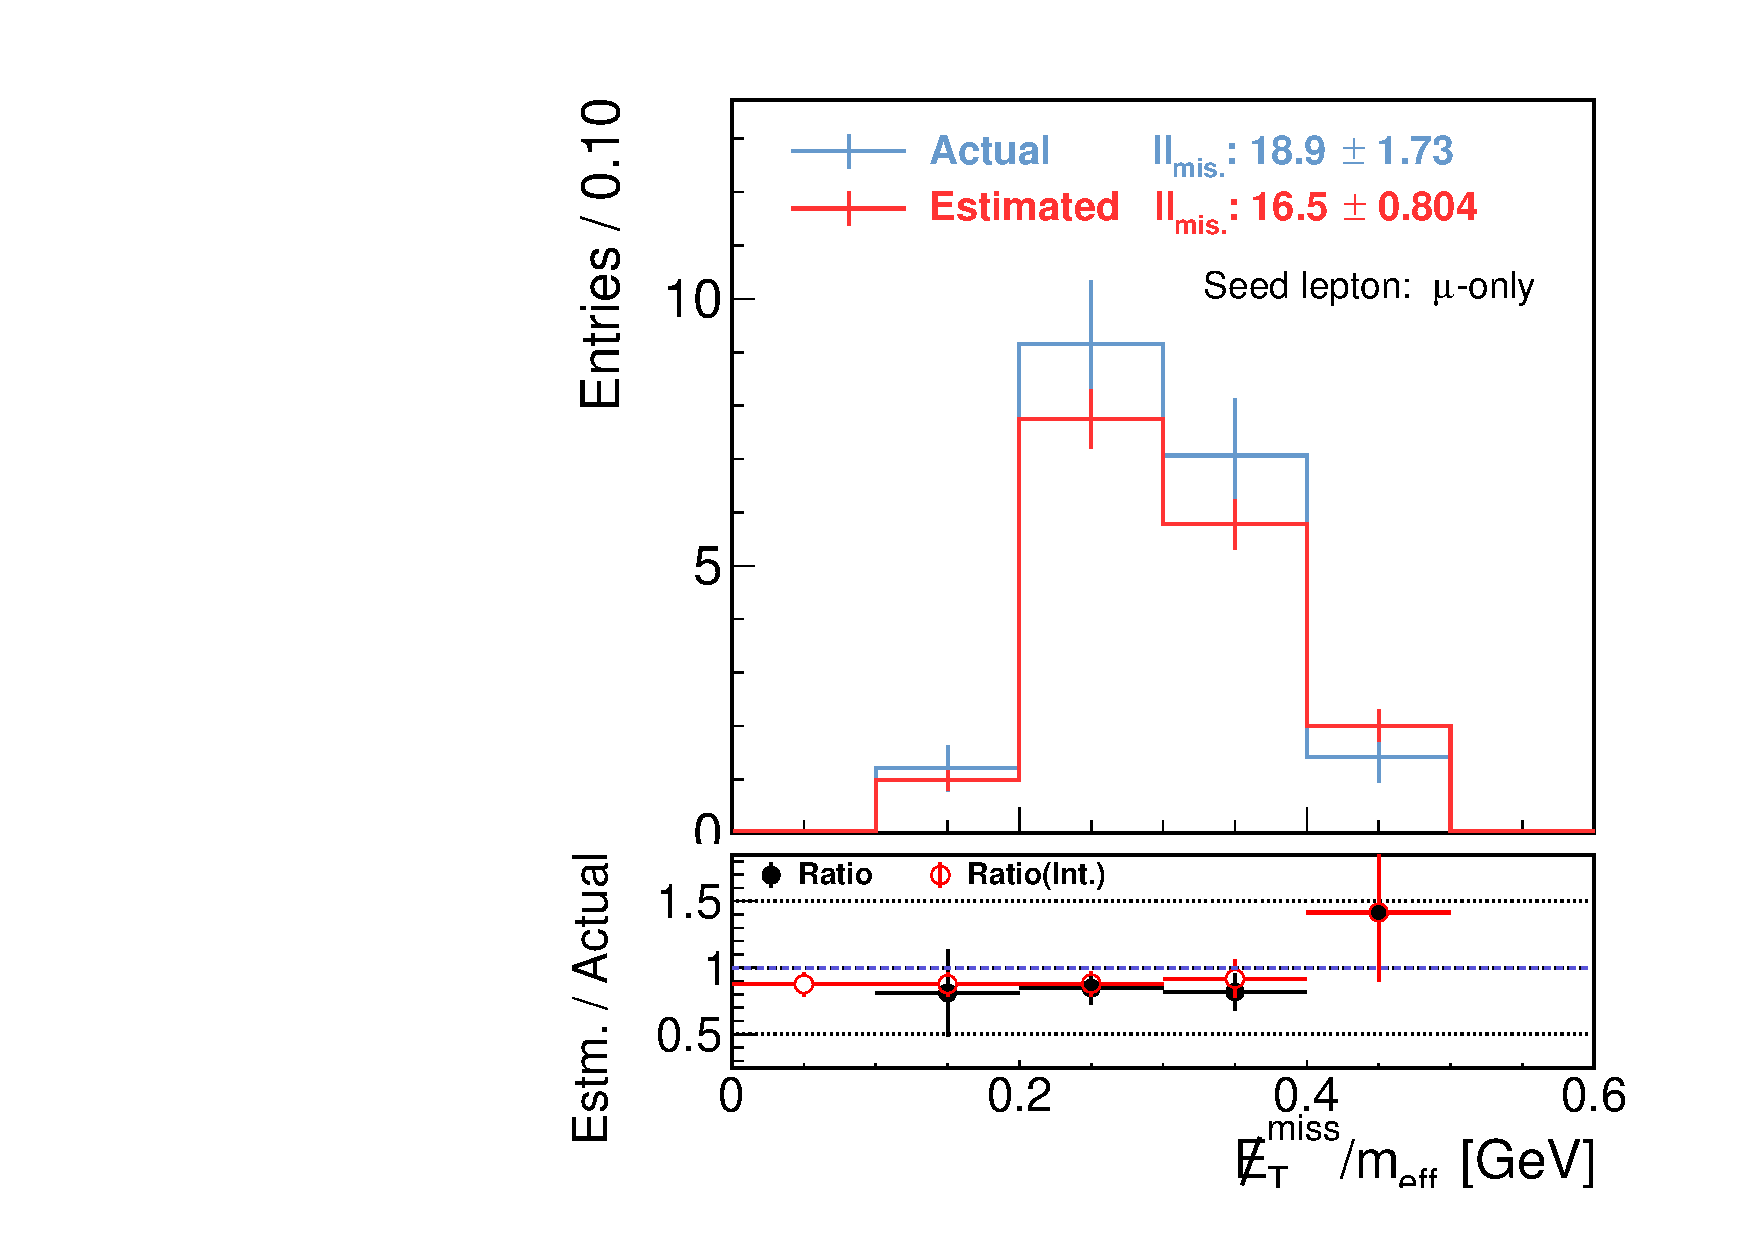
\includegraphics[width=0.32\textwidth]{figures/BGestimation/ObjReplacement/mcClosure_softLep/MisLep_mu_softLep/MisLep_mu_metOverMeff__trMode4_NoSys_softLep.pdf}}
    \subfigure[]{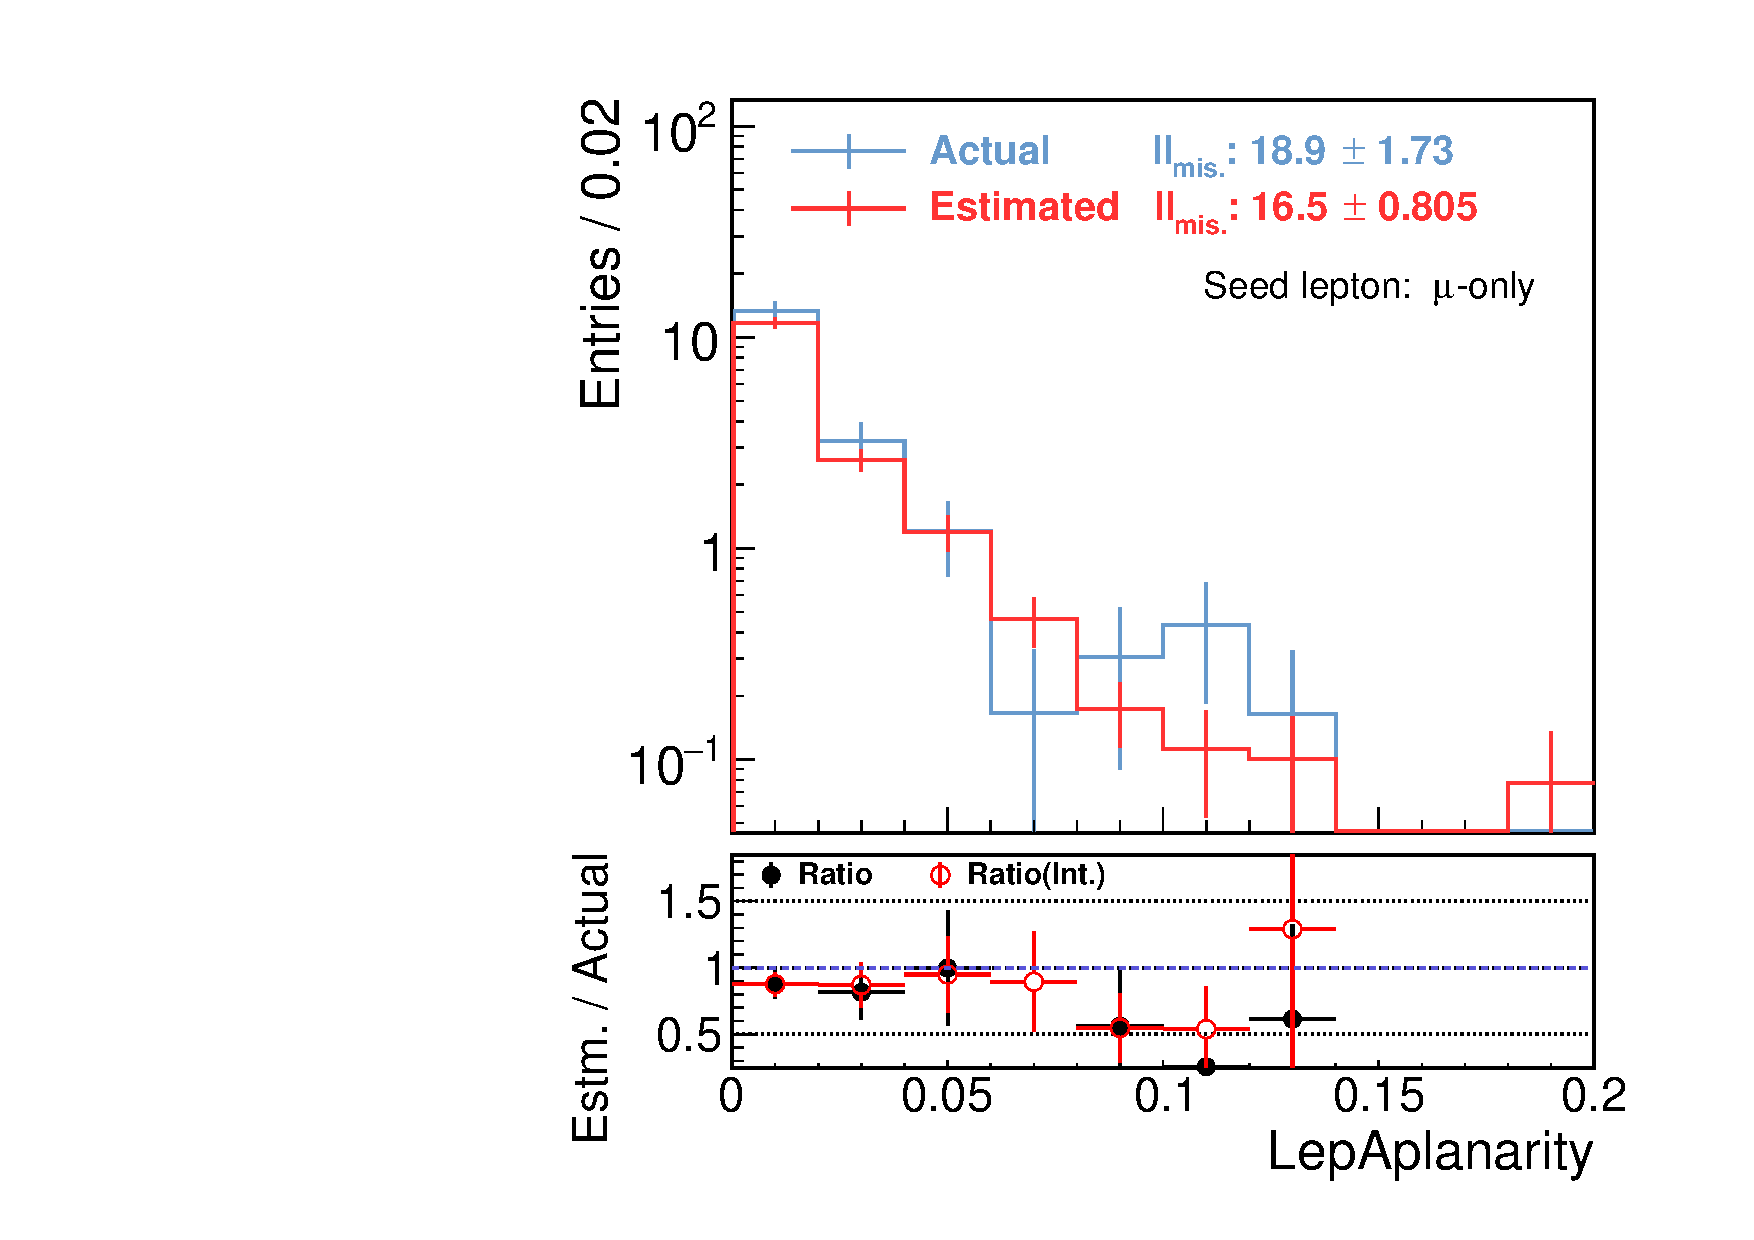
\includegraphics[width=0.32\textwidth]{figures/BGestimation/ObjReplacement/mcClosure_softLep/MisLep_mu_softLep/MisLep_mu_LepAplanarity__trMode4_NoSys_softLep.pdf}}
    \subfigure[]{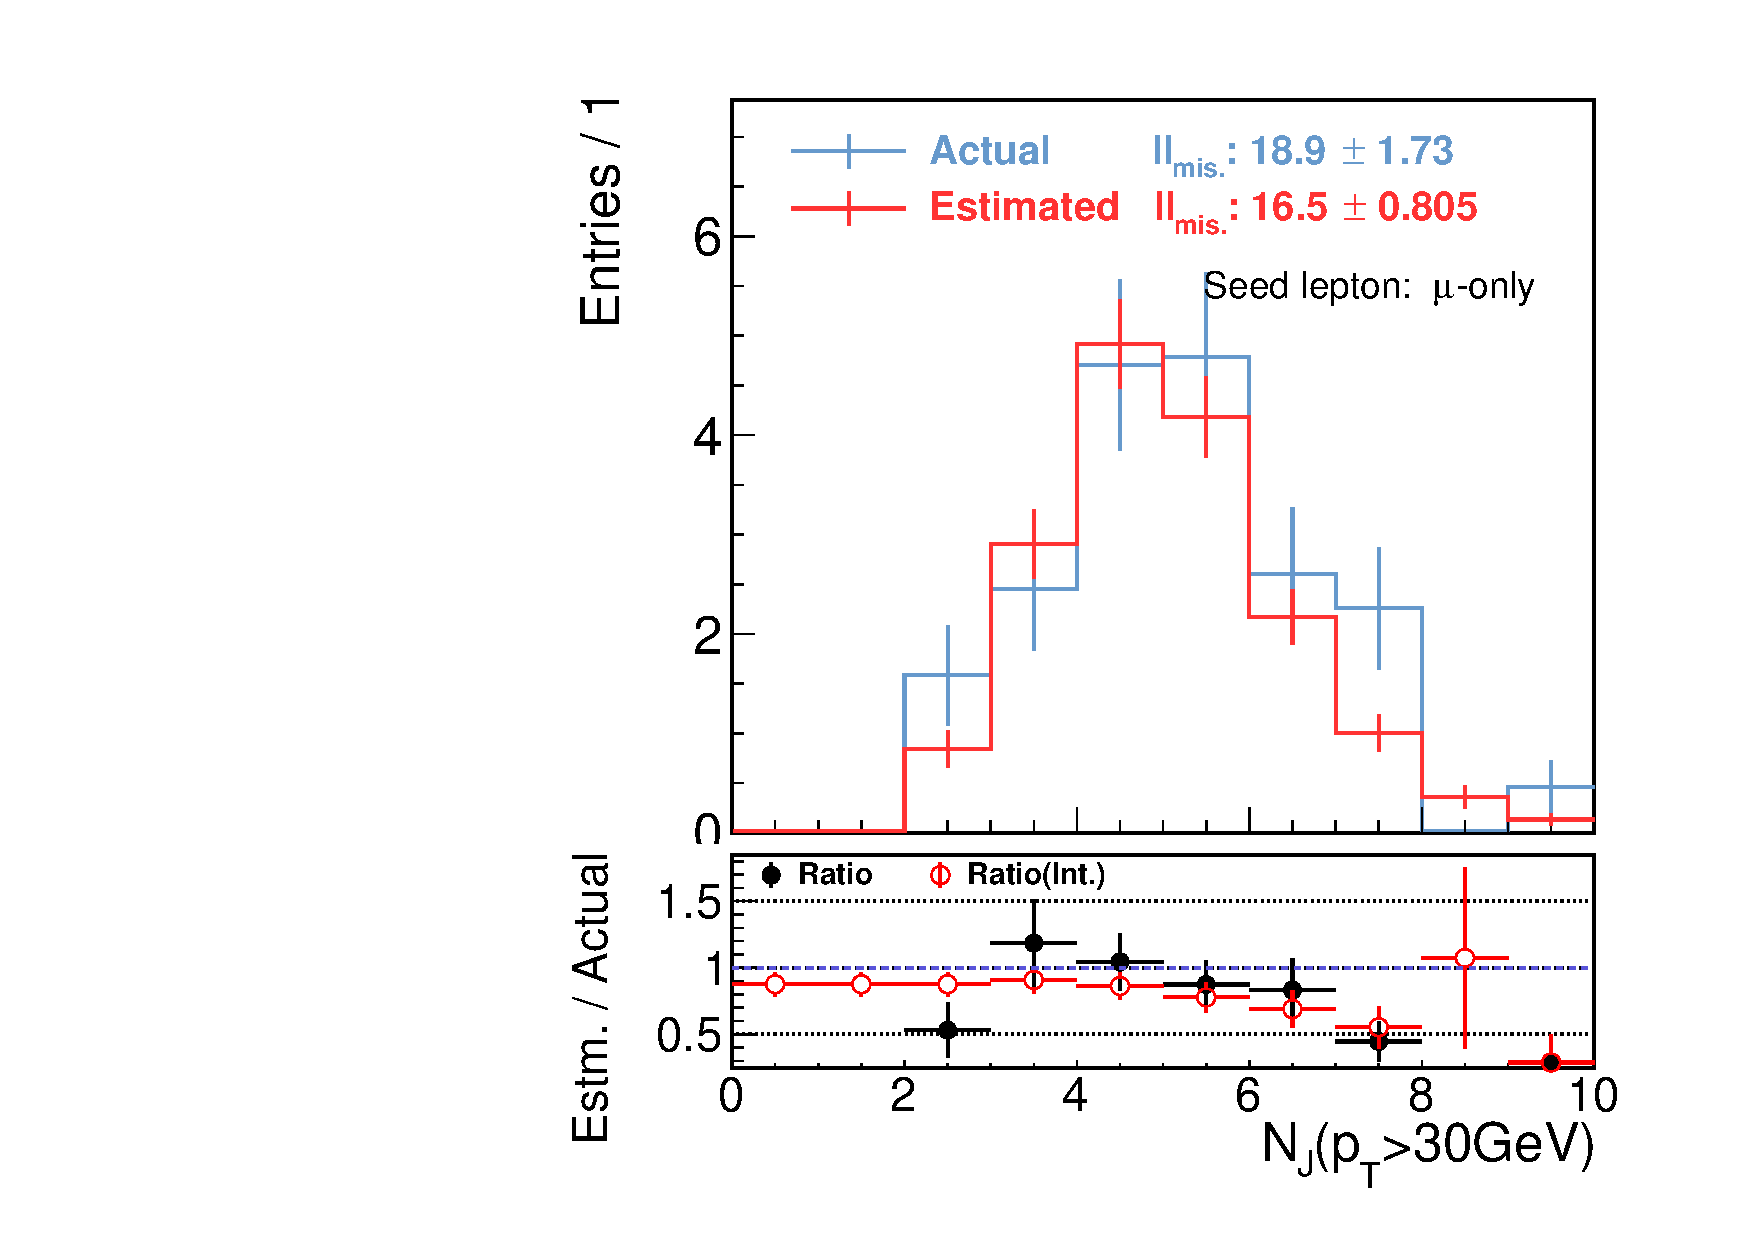
\includegraphics[width=0.32\textwidth]{figures/BGestimation/ObjReplacement/mcClosure_softLep/MisLep_mu_softLep/MisLep_mu_nJet30__trMode4_NoSys_softLep.pdf}}
    \subfigure[]{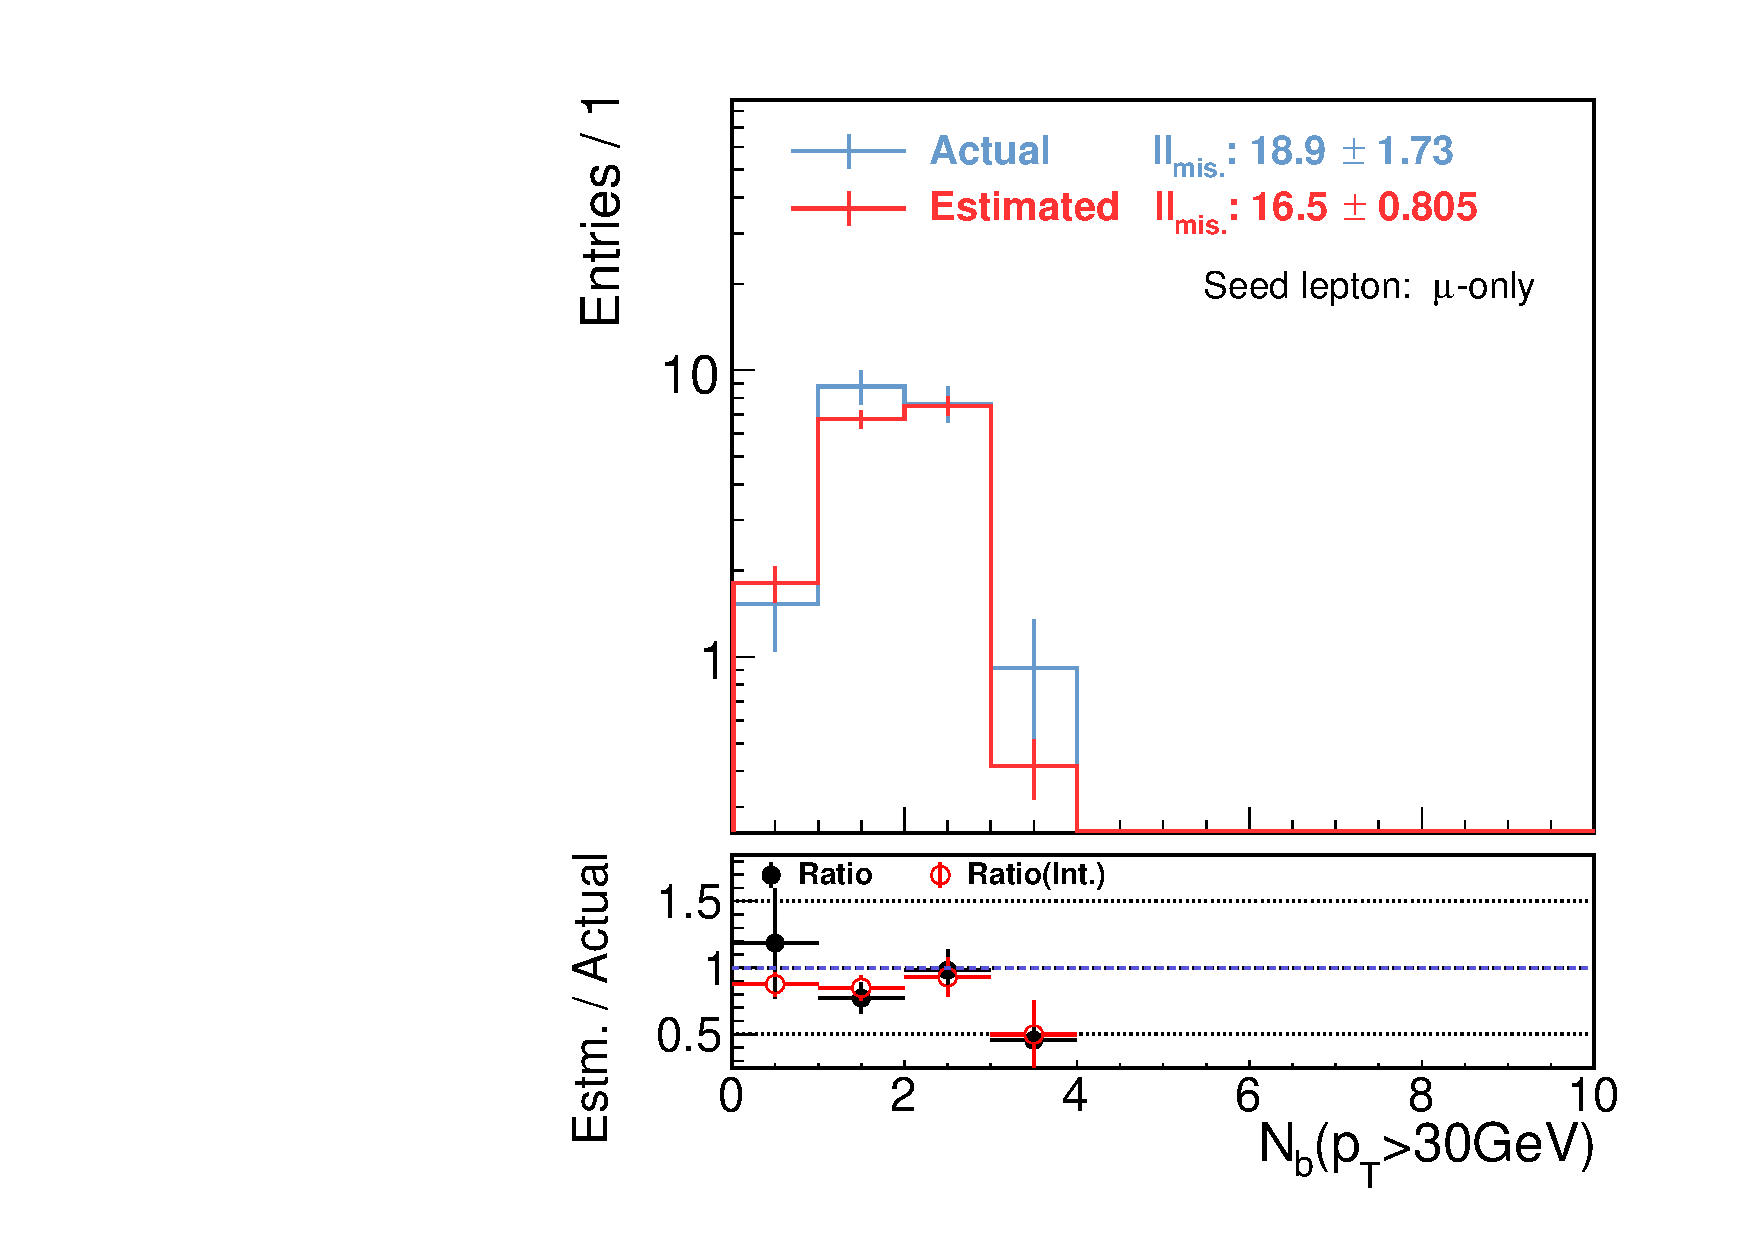
\includegraphics[width=0.32\textwidth]{figures/BGestimation/ObjReplacement/mcClosure_softLep/MisLep_mu_softLep/MisLep_mu_nBJet30__trMode4_NoSys_softLep.pdf}}
    \caption{ MC closure test for \textbf{missing lepton replacement} using $t\bar{t}$ MC sample. Seed events are collected by the use of MET trigger. $p_T<35\gev$ for the leading lepton is required. \textbf{Only muon in the seed events are replaced}. Red points in the bottom plots show the ratio of integrated yields for the two histograms above the x-position that the point indicates. \label{fig::ObjReplace::mcClosure_softLep_MisLep_mu} }
\end{figure}
 %%%%%%%%%%%%%%%%%%%%%%%%%%

%%%%% METHNAME %%%%%%%%%%%%%%%%%%%%%%%%%%
\begin{figure}[h]
  \centering
    \subfig{0.32}{figures/BGestimation/ObjReplacement/mcClosure_softLep/TauRep_emu_softLep/TauRep_emu_jet1Pt__trMode4_NoSys_softLep.pdf}{$\pt$ of leading jet}
    \subfig{0.32}{figures/BGestimation/ObjReplacement/mcClosure_softLep/TauRep_emu_softLep/TauRep_emu_meffInc30__trMode4_NoSys_softLep.pdf}{$\meffInc$}
    \subfig{0.32}{figures/BGestimation/ObjReplacement/mcClosure_softLep/TauRep_emu_softLep/TauRep_emu_met__trMode4_NoSys_softLep.pdf}{$\met$}
    \subfig{0.32}{figures/BGestimation/ObjReplacement/mcClosure_softLep/TauRep_emu_softLep/TauRep_emu_mt__trMode4_NoSys_softLep.pdf}{$\mt$}
    \subfig{0.32}{figures/BGestimation/ObjReplacement/mcClosure_softLep/TauRep_emu_softLep/TauRep_emu_metOverMeff__trMode4_NoSys_softLep.pdf}{$\met/\meffInc$}
    \subfig{0.32}{figures/BGestimation/ObjReplacement/mcClosure_softLep/TauRep_emu_softLep/TauRep_emu_LepAplanarity__trMode4_NoSys_softLep.pdf}{Aplanarity}
    \subfig{0.32}{figures/BGestimation/ObjReplacement/mcClosure_softlep/TauRep_emu_softLep/TauRep_emu_min_dPhi_4j__trMode4_NoSys_softLep.pdf}{$\mindPhiFourJet$}
    \subfig{0.32}{figures/BGestimation/ObjReplacement/mcClosure_softLep/TauRep_emu_softLep/TauRep_emu_nJet30__trMode4_NoSys_softLep.pdf}{Jet multiplicity}
    \subfig{0.32}{figures/BGestimation/ObjReplacement/mcClosure_softLep/TauRep_emu_softLep/TauRep_emu_nBJet30__trMode4_NoSys_softLep.pdf}{$b$-jet multiplicity}
    \caption{ MC closure test for \textbf{tau replacement} using $t\bar{t}$ MC sample. Seed events are collected by the use of MET trigger. $p_T<35\gev$ for the leading lepton is required. \textbf{Both electrons and muons in the seed events are replaced}. Red points in the bottom plots show the ratio of integrated yields for the two histograms above the x-position that the point indicates. \label{fig::ObjReplace::mcClosure_softLep_TauRep_emu} }
\end{figure}
 %%%%%%%%%%%%%%%%%%%%%%%%%%

%%%%%% METHNAME %%%%%%%%%%%%%%%%%%%%%%%%%%
\begin{figure}[h]
  \centering
    \subfigure[]{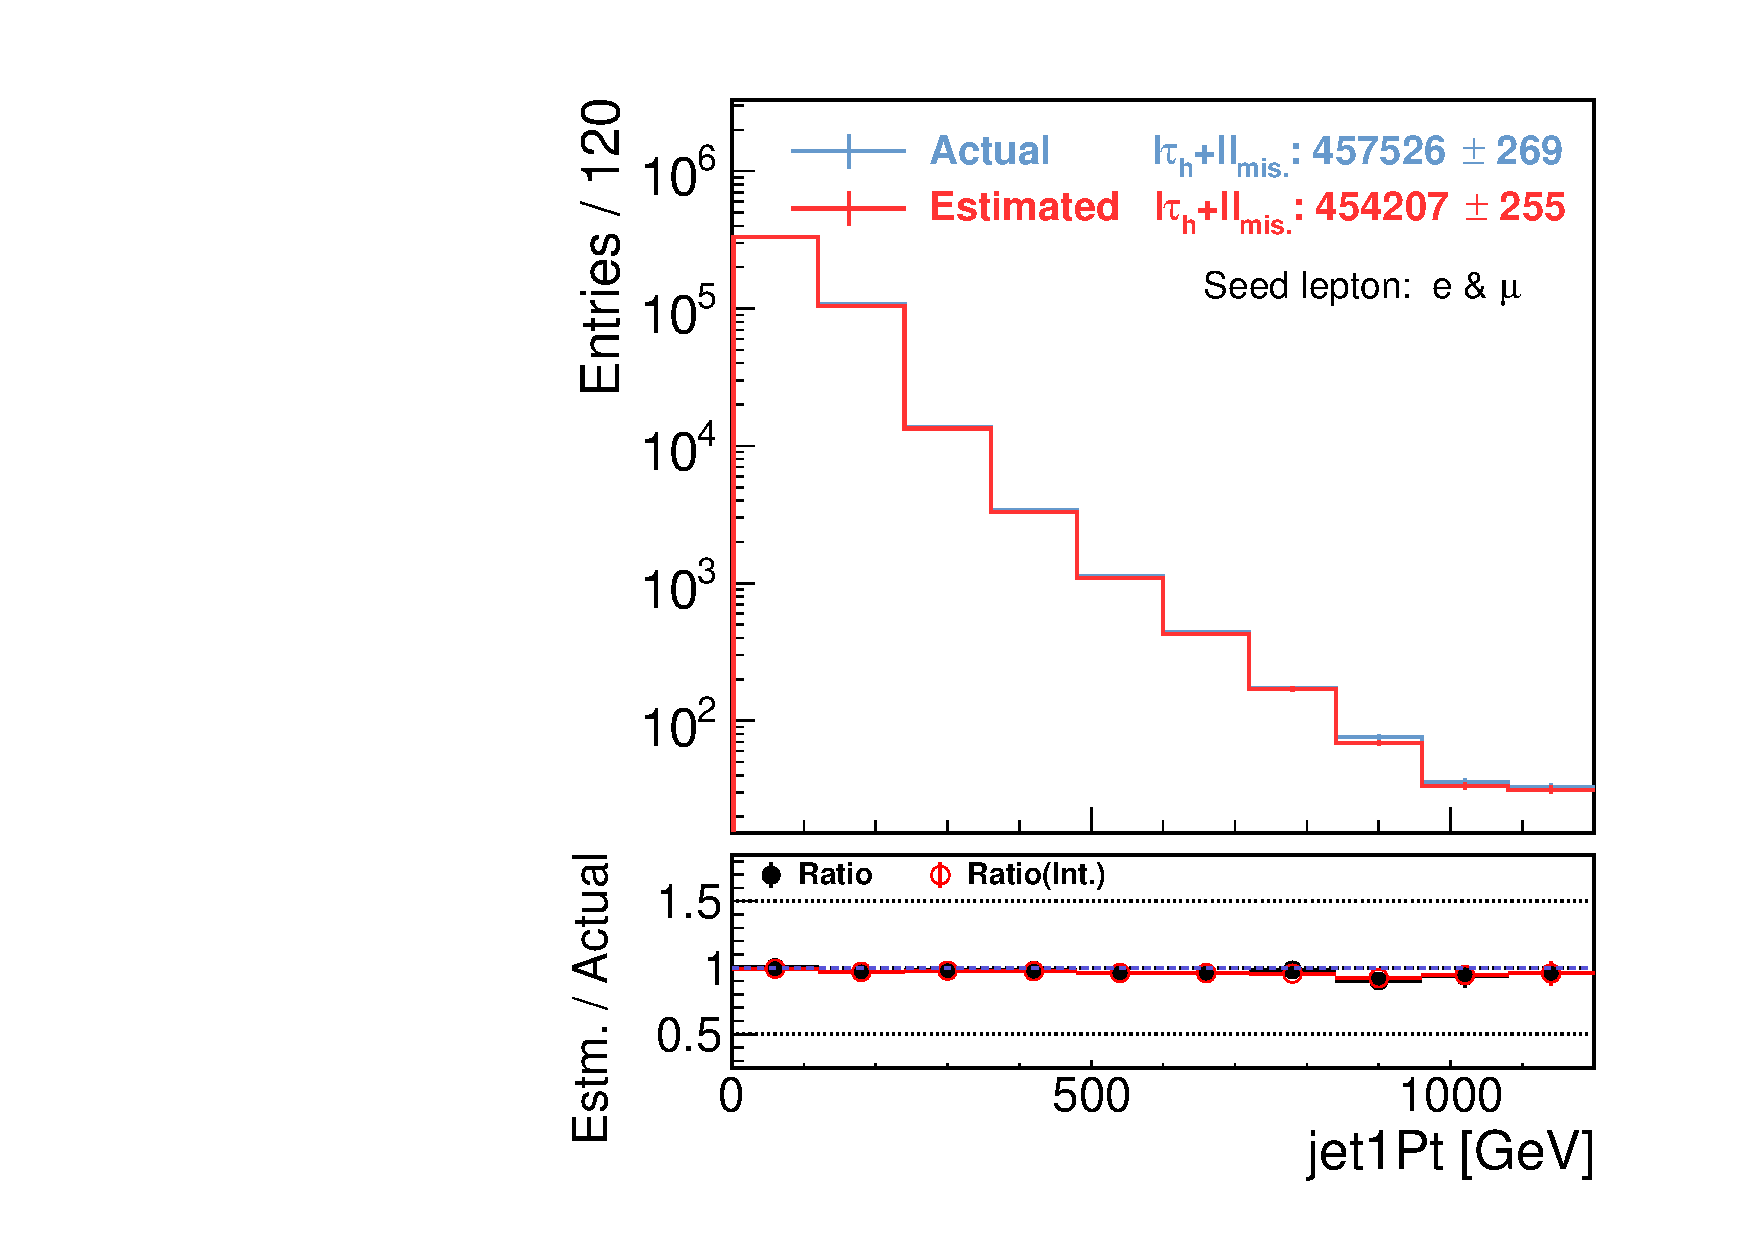
\includegraphics[width=0.32\textwidth]{figures/BGestimation/ObjReplacement/mcClosure/All_emu/All_emu_jet1Pt__trMode4_NoSys.pdf}}
    \subfigure[]{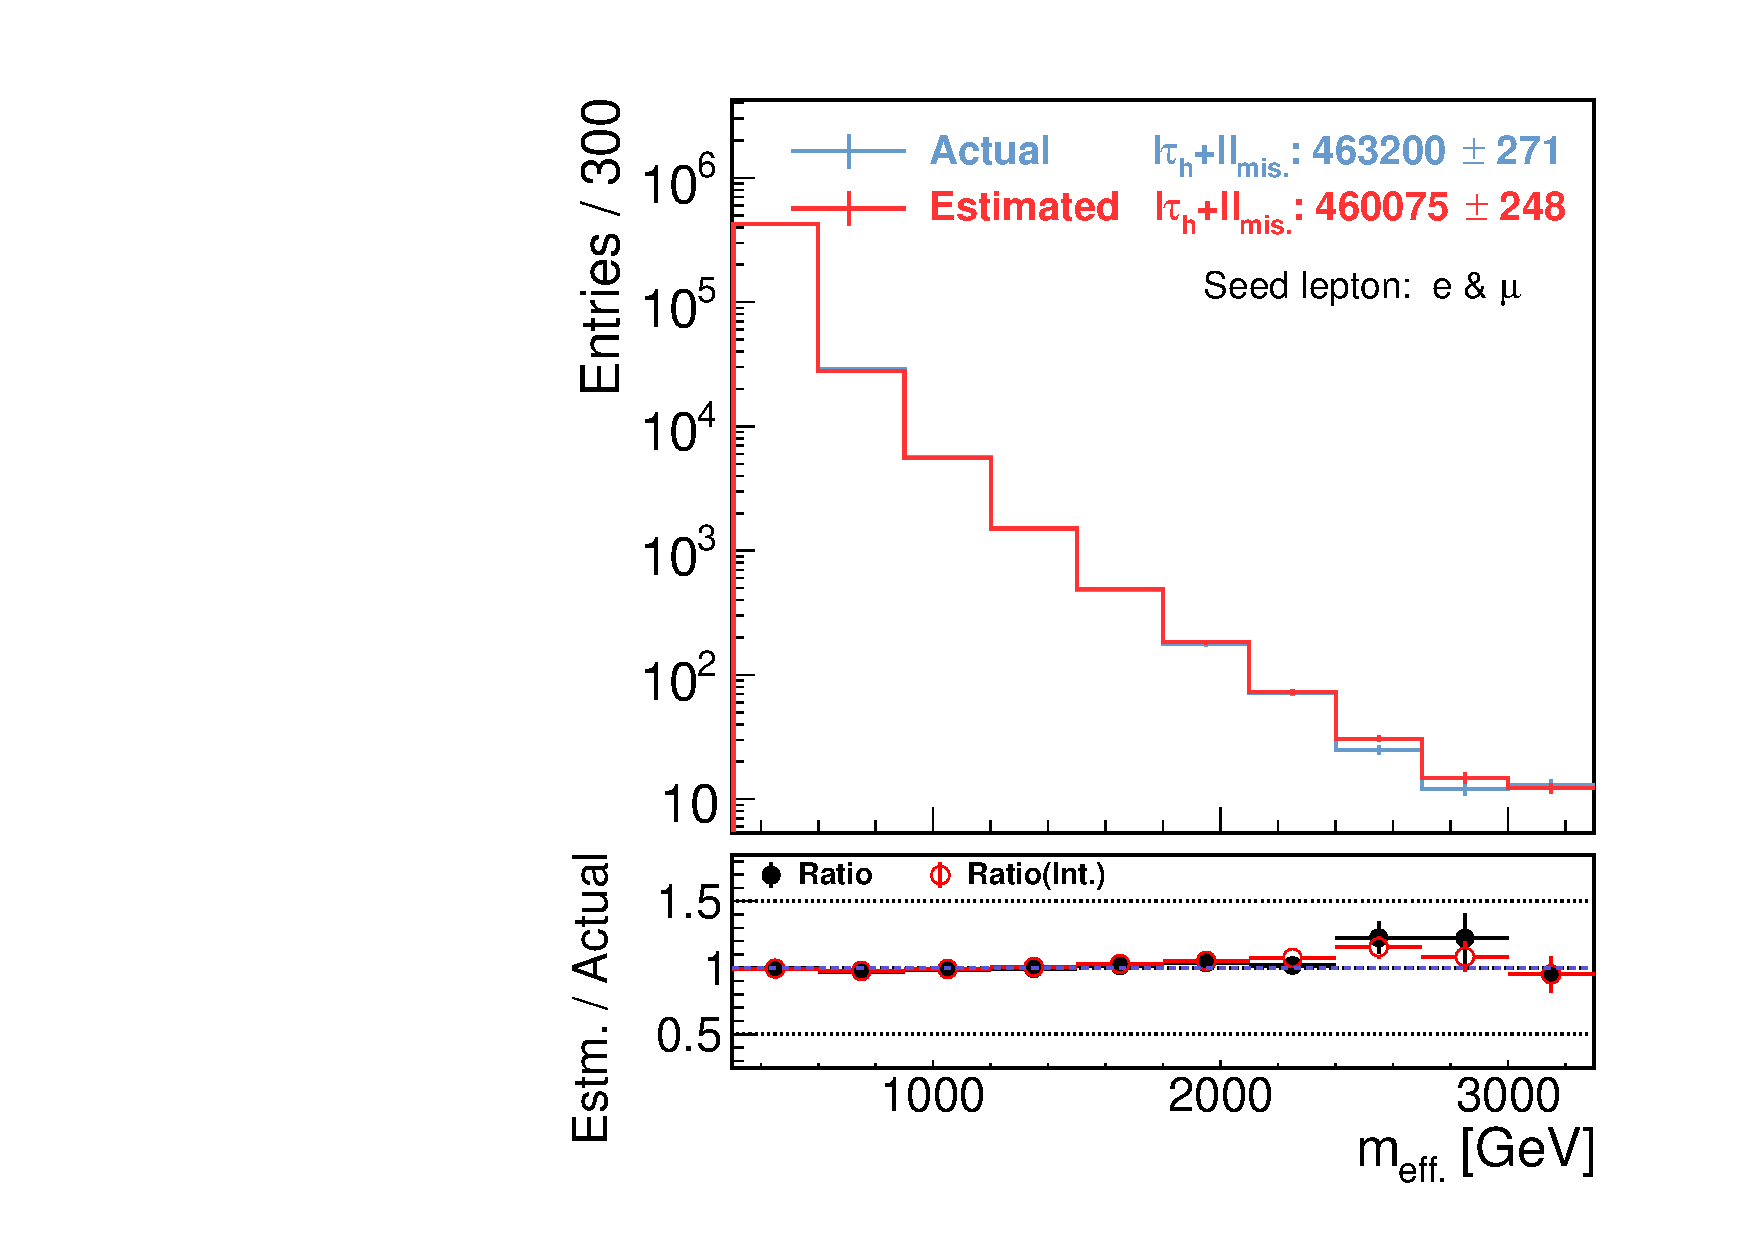
\includegraphics[width=0.32\textwidth]{figures/BGestimation/ObjReplacement/mcClosure/All_emu/All_emu_meffInc30__trMode4_NoSys.pdf}}
    \subfigure[]{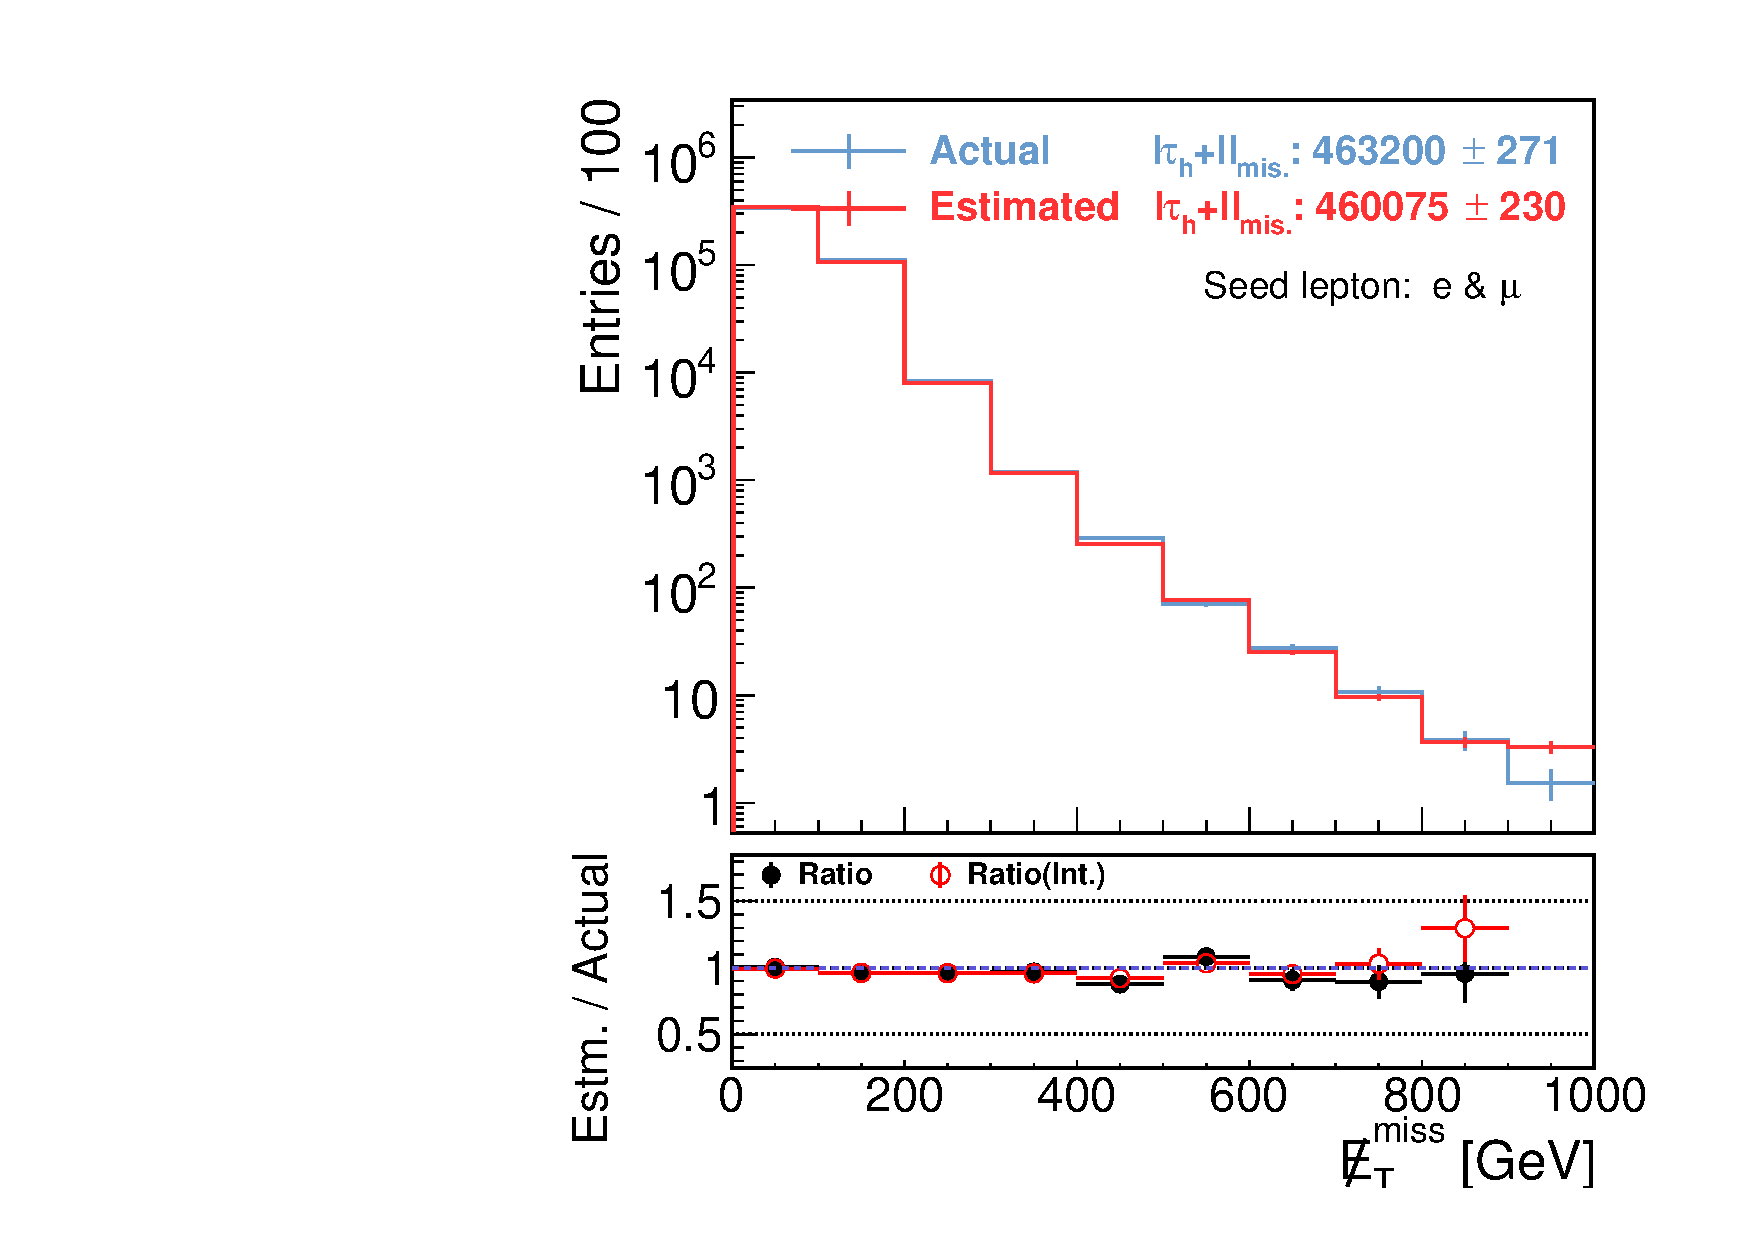
\includegraphics[width=0.32\textwidth]{figures/BGestimation/ObjReplacement/mcClosure/All_emu/All_emu_met__trMode4_NoSys.pdf}}
    \subfigure[]{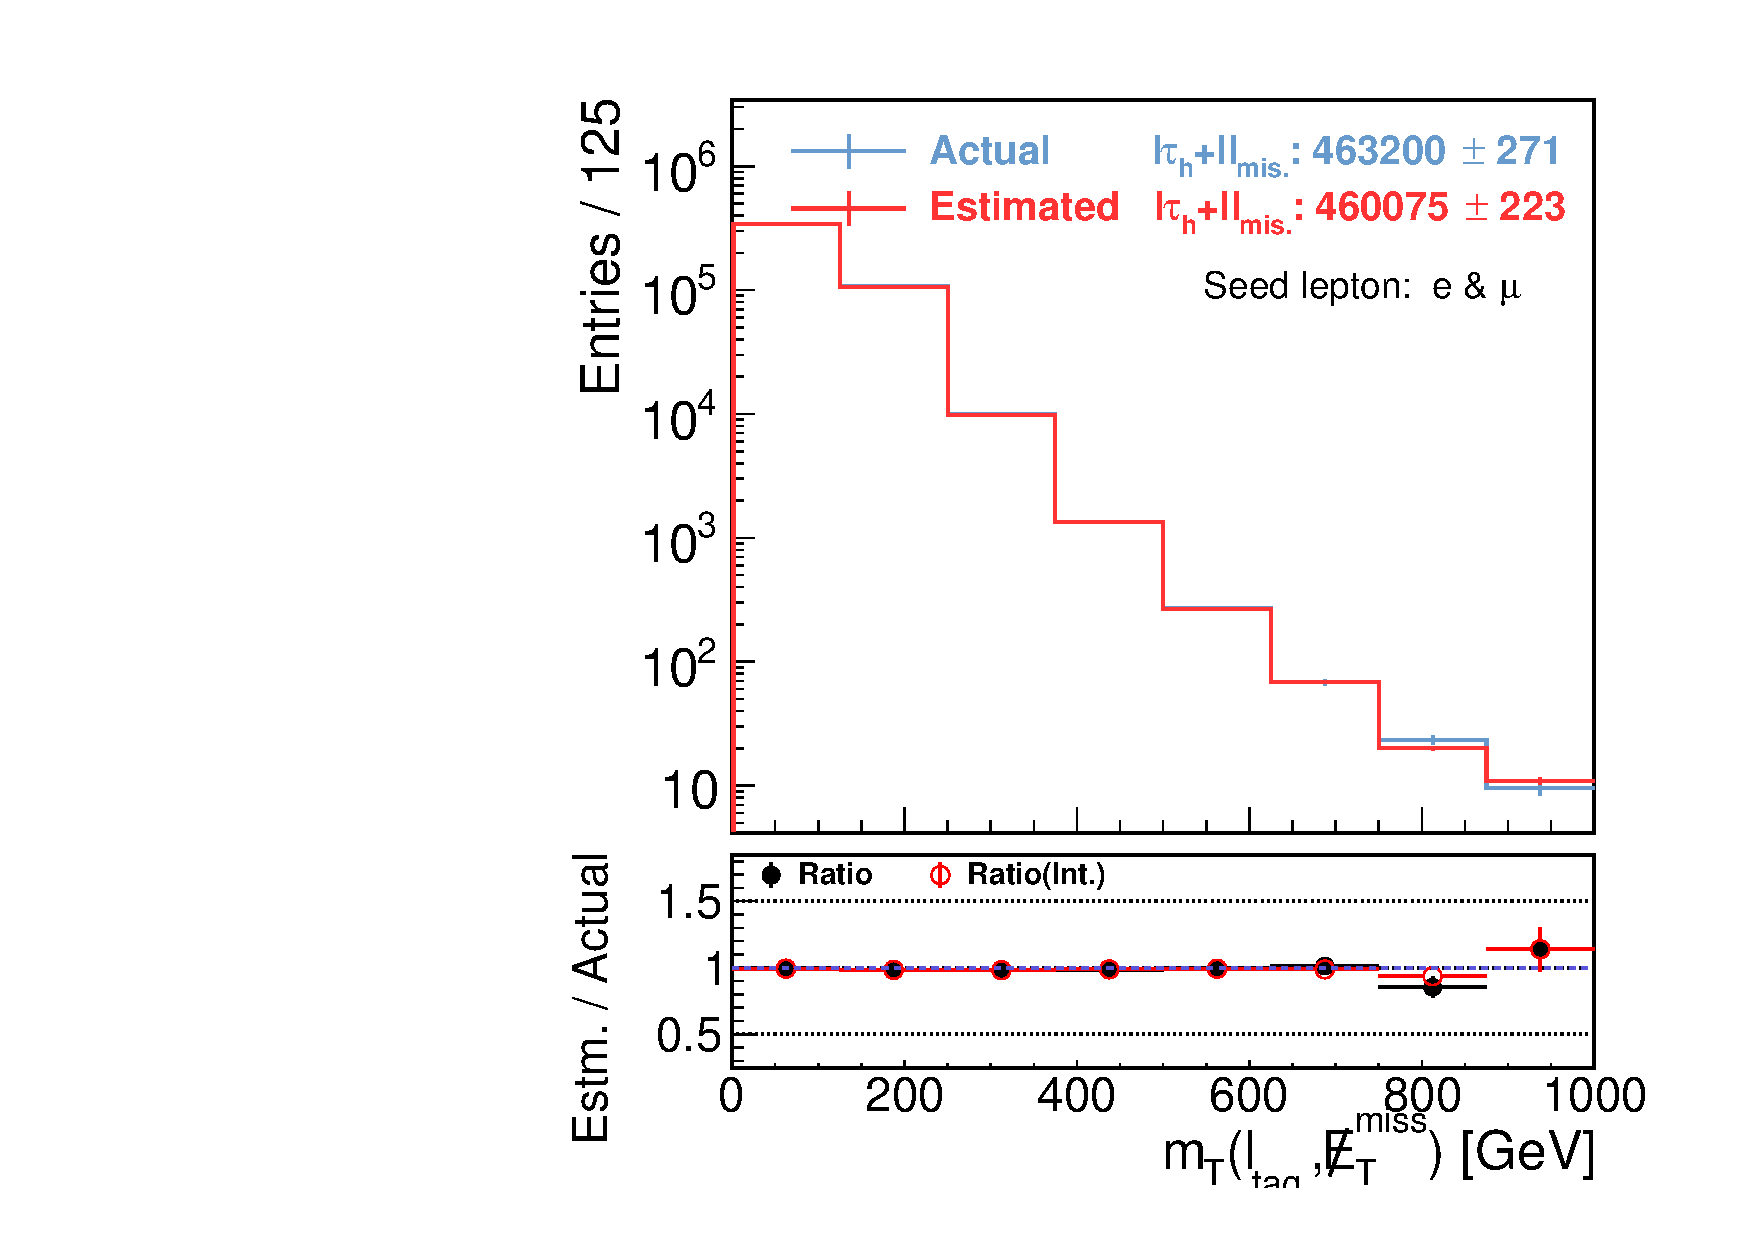
\includegraphics[width=0.32\textwidth]{figures/BGestimation/ObjReplacement/mcClosure/All_emu/All_emu_mt__trMode4_NoSys.pdf}}
    \subfigure[]{\includegraphics[width=0.32\textwidth]{figures/BGestimation/ObjReplacement/mcClosure/All_emu/All_emu_tagLepPt__trMode4_NoSys.pdf}}
    \subfigure[]{\includegraphics[width=0.32\textwidth]{figures/BGestimation/ObjReplacement/mcClosure/All_emu/All_emu_metOverMeff__trMode4_NoSys.pdf}}
    \subfigure[]{\includegraphics[width=0.32\textwidth]{figures/BGestimation/ObjReplacement/mcClosure/All_emu/All_emu_LepAplanarity__trMode4_NoSys.pdf}}
    \subfigure[]{\includegraphics[width=0.32\textwidth]{figures/BGestimation/ObjReplacement/mcClosure/All_emu/All_emu_nJet30__trMode4_NoSys.pdf}}
    \subfigure[]{\includegraphics[width=0.32\textwidth]{figures/BGestimation/ObjReplacement/mcClosure/All_emu/All_emu_nBJet30__trMode4_NoSys.pdf}}
    \caption{ MC closure test for \textbf{combined estimation of missing lepton rep. and tau rep.} using $t\bar{t}$ MC sample. Seed events are collected by the single-lepton trigger. $p_T>35\gev$ for the leading lepton is required. \textbf{Both electrons and muons in the seed events are replaced}. Red points in the bottom plots show the ratio of integrated yields for the two histograms above the x-position that the point indicates. \label{fig::ObjReplace::mcClosure_All_emu} }
\end{figure}
 %%%%%%%%%%%%%%%%%%%%%%%%%%


Closure is generally good. Non-closure is typically within $10\%$ ($5\%$), and never exceeds $30\%$ ($10\%$) significantly for the missing lepton replacement (the tau replacement).
The closure of missing lepton replacement is generally worse than that of tau replacement, however it is not worrisome since the contribution of $\ell\ell_{\mathrm{mis.}}$ is typically $5\sim10$ times smaller than $\ell\tau_{\mathrm{h}}$ in our signal regions. \\


\clearpage
\subsubsection{Source of non-closure} \label{sec::ObjReplace::NonClosure} 
Visible non-closures are found in some distributions such as MET and jetPt etc. These are mainly due to following reasons:

\begin{description}
\item [Kinematical bias triggered by the two lepton requirement in seed event selection (All)] \mbox{} \\
Since objects decaying from heavily boosted particles get collimated and overlapped each other, offline selection efficiency for leptons (either eff. of reconstruction, ID, and overlap-removal) is generally deteriorated in phase space with hard kinematics. This is in the same time means that selecting events with exactly two offline leptons already biases the kinematics, since the events in the ``boosted topology'' tends to be discarded. Therefore spectra estimated by 2 lepton seed events will be generally softer. Electrons address larger effect because the efficiency drop in the boosted environment is more severe than muons (plots will come later).

\if 0
Fig \ref{fig::ObjReplace::mcClosure::biasFrom2Lreq} show the explicit comparison of $t\bar{t}$ kinematics of events passing or failing the offline selection.

% -------------- mcClosure::biasFrom2LSelection
In both methods, the primary source of non-closure originated from ...
\begin{figure}[h]
  \centering
    \subfigure[]{\includegraphics[width=0.3\textwidth]{figures/BGestimation/ObjReplacement/mcClosure/source_nonClosure/biasFrom2Lreq/tr_b1Pt_2Lvs1L_tagMu_varElConeOR.eps}}
    \subfigure[]{\includegraphics[width=0.3\textwidth]{figures/BGestimation/ObjReplacement/mcClosure/source_nonClosure/biasFrom2Lreq/tr_t1Pt_2Lvs1L_tagMu_varElConeOR.eps}}
    \subfigure[]{\includegraphics[width=0.3\textwidth]{figures/BGestimation/ObjReplacement/mcClosure/source_nonClosure/biasFrom2Lreq/tr_ttPt_2Lvs1L_tagMu_varElConeOR.eps}}
    \subfigure[]{\includegraphics[width=0.3\textwidth]{figures/BGestimation/ObjReplacement/mcClosure/source_nonClosure/biasFrom2Lreq/tr_b1Pt_2Lvs1L_tagEl_varElConeOR.eps}}
    \subfigure[]{\includegraphics[width=0.3\textwidth]{figures/BGestimation/ObjReplacement/mcClosure/source_nonClosure/biasFrom2Lreq/tr_t1Pt_2Lvs1L_tagEl_varElConeOR.eps}}
    \subfigure[]{\includegraphics[width=0.3\textwidth]{figures/BGestimation/ObjReplacement/mcClosure/source_nonClosure/biasFrom2Lreq/tr_ttPt_2Lvs1L_tagEL_varElConeOR.eps}}
%%
%    \subfigure[]{\includegraphics[width=0.3\textwidth]{figures/BGestimation/ObjReplacement/mcClosure/source_nonClosure/biasFrom2Lreq/tr_b1Pt_2LvsLtauh_tagMu_varElConeOR.eps}}
%    \subfigure[]{\includegraphics[width=0.3\textwidth]{figures/BGestimation/ObjReplacement/mcClosure/source_nonClosure/biasFrom2Lreq/tr_t1Pt_2LvsLtauh_tagMu_varElConeOR.eps}}
%    \subfigure[]{\includegraphics[width=0.3\textwidth]{figures/BGestimation/ObjReplacement/mcClosure/source_nonClosure/biasFrom2Lreq/tr_ttPt_2LvsLtauh_tagMu_varElConeOR.eps}}
%    \subfigure[]{\includegraphics[width=0.3\textwidth]{figures/BGestimation/ObjReplacement/mcClosure/source_nonClosure/biasFrom2Lreq/tr_b1Pt_2LvsLtauh_tagEl_varElConeOR.eps}}

%    \subfigure[]{\includegraphics[width=0.3\textwidth]{figures/BGestimation/ObjReplacement/mcClosure/source_nonClosure/biasFrom2Lreq/tr_t1Pt_2LvsLtauh_tagEl_varElConeOR.eps}}
%    \subfigure[]{\includegraphics[width=0.3\textwidth]{figures/BGestimation/ObjReplacement/mcClosure/source_nonClosure/biasFrom2Lreq/tr_ttPt_2LvsLtauh_tagEL_varElConeOR.eps}}
    \caption{Comparison of di-leptonic $t\bar{t}$ kinematics with various offline selections. Only $e\mu$ are used for simplicity. Black lines show the kinematics of events with exactly two baseline leptons (``2 baseLep''), while the purple lines are case with events failing the requirement (``1 baseXX + 1 missing YY''). The other colors are the breakdown of purple ones by different causes of ``missing''. All histograms in the top raws are normalized to unity. Bottom raws are the ratio with respect to ``2 baseLep'' from which we can see    \label{fig::ObjReplace::mcClosure::biasFrom2Lreq} }
\end{figure}
\fi

% -------------- mcClosure::metSoftTerm
\item [Too rough treatment of MET soft term for missing muon (missing muon replacement)]  \mbox{} \\
Currently missing muons are completely regarded as invisible particles and their 4-vector are naively added in MET recalculation, while in reality their contribution are more likely to be counted in the MET track soft term. This inconsistent modeling is supposed to be the dominant source of non-closure in MET related variables in the missing muon replacement. Naively thinking, this can be improved by simply adding the missing muons into the track soft term. However this seems not the case according to \ref{fig::ObjReplace::mcClosure::metSoftTerm_mu}. The reason has not been fully understood, but it is perhaps due to the bad resolution of muon tracks added into TST.

\begin{figure}[h]
  \centering
    \subfigure[]{\includegraphics[width=0.3\textwidth]{figures/BGestimation/ObjReplacement/mcClosure/source_nonClosure/metSoftTerm/MisLep_mu_met.eps}}
    \subfigure[]{\includegraphics[width=0.3\textwidth]{figures/BGestimation/ObjReplacement/mcClosure/source_nonClosure/metSoftTerm/InclSoftTerm_MisLep_mu_met.eps}}
    \caption{Closure in MET distrubution. (a) Default treatment of missing muon (cound as invisible). (b) Always add missing muons in the TST.  \label{fig::ObjReplace::mcClosure::metSoftTerm_mu} }
\end{figure}


% -------------- mcClosure::polCorrection
\item [Wrong assumption on tau polarization (tau replacement)] \mbox{} \\
For technical simplicity, tau leptons are assumed to be unpolarized during the decay. This is of course not true as tau leptons are usually generated through weak decay of W-bosons. In the tau replacement, the MC non-closure in MET (and $m_{\mathrm{T}}$ etc.) is understood by this polarization effect. Fig. \ref{fig::ObjReplace::mcClosure::rwgt_x} and fig. \ref{fig::ObjReplace::mcClosure::rwgt_x_mt} describe a test of reweighting in terms of visible tau fraction $x := E(\tau_{h})/E(\tau)$, known as a variable sensitive to the polarization of parent tau, where the closure successfully recover. Although this $x$-reweighting correction works quite nicely, given the impact of this non-closure is marginal in our signal regions ($<5\%$), we decided not to apply any corrections to avoid further complexity of the method.

\begin{figure}[h]
  \centering
    \subfigure[]{\includegraphics[width=0.3\textwidth]{figures/BGestimation/ObjReplacement/mcClosure/source_nonClosure/taupol/TauRep_emu_tr_hadTau_x.eps}}
    \subfigure[]{\includegraphics[width=0.3\textwidth]{figures/BGestimation/ObjReplacement/mcClosure/source_nonClosure/taupol/rwgt_x_TauRep_emu_tr_hadTau_x.eps}}
    \subfigure[]{\includegraphics[width=0.35\textwidth]{figures/BGestimation/ObjReplacement/mcClosure/source_nonClosure/taupol/fit_hadtaux.eps}}
    \caption{Reweighting in terms of the visible tau fraction $x := E(\tau_{h})/E(\tau)$. (a) $x$ distribution before the reweighting , (b) $x$ distribution after the reweighting. (c) An ad hoc fit of the reweighting function by third order polynomial. The reweighting function is almost invariant in terms of phase space.  \label{fig::ObjReplace::mcClosure::rwgt_x} }
\end{figure}

\begin{figure}[h]
  \centering
    \subfigure[]{\includegraphics[width=0.24\textwidth]{figures/BGestimation/ObjReplacement/mcClosure/source_nonClosure/taupol/TauRep_emu_mt.eps}}
    \subfigure[]{\includegraphics[width=0.24\textwidth]{figures/BGestimation/ObjReplacement/mcClosure/source_nonClosure/taupol/rwgt_x_TauRep_emu_mt.eps}}
    \subfigure[]{\includegraphics[width=0.24\textwidth]{figures/BGestimation/ObjReplacement/mcClosure/source_nonClosure/taupol/TauRep_emu_met.eps}}
    \subfigure[]{\includegraphics[width=0.24\textwidth]{figures/BGestimation/ObjReplacement/mcClosure/source_nonClosure/taupol/rwgt_x_TauRep_emu_met.eps}}
    \caption{ (a) $m_{\mathrm{T}}$ and (c) MET distribution before the reweighting in $x$, and (b)(d) after the reweighting.  \label{fig::ObjReplace::mcClosure::rwgt_x_mt} }
\end{figure}

%\begin{figure}[h]
%  \centering

%\end{figure}

\end{description}


\clearpage

%\clearpage
\subsubsection{Closuer test with tigher selection} \label{sec::ObjReplace::mcClosure_tight} 
Closure tests are also performed in phase space close to signal regions. Fig. \ref{fig::ObjReplace::mcClosure::MisLep_regionYieldsBT} $\sim$ \ref{fig::ObjReplace::mcClosure::MisLepTauRep_regionYieldsBV} are the btag/bveto-splitted closure in various regions requiring high MET, $m_{T}$, $m_{\mathrm{eff.}}$ etc. The non-closure stay within 30$\%$ (10$\%$) for the missing lepton replacement (the tau replacement).\\

% -------------- mcClosure::MisLep_regionYields
\begin{figure}[htbp]
  \begin{center}
    \includegraphics[width=160mm]{figures/BGestimation/ObjReplacement/mcClosure/MisLep_emu/MisLep_emu_regionYieldsBT__trMode4_NoSys.eps}
    \captionof{figure}{MC closure test for \textbf{missing lepton replacement} in SR-like \textbf{b-tagged} regions. Pre-selection $p_{T}(\ell_{1})>35\gev$ is applied on top of the cuts noted by the labels.}
    \label{fig::ObjReplace::mcClosure::MisLep_regionYieldsBT}
%%
    \includegraphics[width=160mm]{figures/BGestimation/ObjReplacement/mcClosure/MisLep_emu/MisLep_emu_regionYieldsBV__trMode4_NoSys.eps}
    \captionof{figure}{MC closure test for \textbf{missing lepton replacement} in SR-like \textbf{b-vetoed} regions. Pre-selection $p_{T}(\ell_{1})>35\gev$ is applied on top of the cuts noted by the labels.}
    \label{fig::ObjReplace::mcClosure::MisLep_regionYieldsBV}
  \end{center}
\end{figure}
%-------------------------------
% -------------- mcClosure::TauRep_regionYields
\begin{figure}[htbp]
  \begin{center}
    \includegraphics[width=160mm]{figures/BGestimation/ObjReplacement/mcClosure/TauRep_emu/TauRep_emu_regionYieldsBT__trMode4_NoSys.eps}
    \captionof{figure}{MC closure test for \textbf{tau replacement} in SR-like \textbf{b-tagged} regions. Pre-selection $p_{T}(\ell_{1})>35\gev$ is applied on top of the cuts noted by the labels.}
    \label{fig::ObjReplace::mcClosure::TauRep_regionYieldsBT}
%%
    \includegraphics[width=160mm]{figures/BGestimation/ObjReplacement/mcClosure/TauRep_emu/TauRep_emu_regionYieldsBV__trMode4_NoSys.eps}
    \captionof{figure}{MC closure test for \textbf{tau replacement} in SR-like \textbf{b-vetoed} regions. Pre-selection $p_{T}(\ell_{1})>35\gev$ is applied on top of the cuts noted by the labels.}
    \label{fig::ObjReplace::mcClosure::TauRep_regionYieldsBV}
  \end{center}
\end{figure}
%-------------------------------
% -------------- mcClosure::MisLep+TauReo_regionYields
\begin{figure}[htbp]
  \begin{center}
    \includegraphics[width=160mm]{figures/BGestimation/ObjReplacement/mcClosure/All_emu/All_emu_regionYieldsBT__trMode4_NoSys.eps}
    \captionof{figure}{MC closure test for \textbf{combined estimation of missing-lep. rep. and tau replacement} in SR-like \textbf{b-tagged} regions. Pre-selection $p_{T}(\ell_{1})>35\gev$ is applied on top of the cuts noted by the labels.}
    \label{fig::ObjReplace::mcClosure::MisLepTauRep_regionYieldsBT}
%%
    \includegraphics[width=160mm]{figures/BGestimation/ObjReplacement/mcClosure/All_emu/All_emu_regionYieldsBV__trMode4_NoSys.eps}
    \captionof{figure}{MC closure test for \textbf{combined estimation of missing-lep. rep. and tau replacement} in SR-like \textbf{b-vetoed} regions. Pre-selection $p_{T}(\ell_{1})>35\gev$ is applied on top of the cuts noted by the labels.}
    \label{fig::ObjReplace::mcClosure::MisLepTauRep_regionYieldsBV}
  \end{center}
\end{figure}
%-------------------------------


%%%%%%%%%%%%%%%%%%%%%%%%%%%%%%%%%%%%%%%%%%%%%%%%%%

%%%%%%%%%%%%%%%%%%%%%%%%%% Data Closure test %%%%%%%%%%%%%%%%%%%%%%%%%%%%%%%%
\clearpage
\subsection{Closure test using data in 1-lepton validation regions.} \label{sec::ObjReplace::dataClosure}
The method is also validated by data using 1L validation regions (1LVRs) dominated by $\ell\ell_{\mathrm{mis.}}$ and $\ell\tau_{\mathrm{h}}$. \\
There are two procedures to be implemented additionally when moving from MC closure test to application to data:

\begin{description}
\item [Subtraction of irrelevant component] \mbox{} \\
As it is impossible to know the BG species in a single data event, some of events from irrelevant processes ($W$+jets etc.) in 2LCR are inevitably undergo the replacement, generating "fake" sub-events which no processes in 1L regions correspond to. This contribution has to be removed using the knowledge of MC.
The example of relevant and irrelevant processes are summarized in tab.\ref{tab::ObjReplace::dataClosure::BGspecies}. Basically processes with exactly two leptons are "relevant", except for $\ell\tau, \tau\rightarrow \ell\nu\nu$ ($\ell\tau_{\ell}$) and $Z\rightarrow\ell\ell$.\\
$\ell\tau_{\ell}$ is the largest component to be subtracted in the tau replacement ($10\%\sim20\%$). As the impact of MC mis-modeling is usually non-negligible, the ratio to the contribution from relevant components are taken from MC, instead of the absolute yield, to avoid the direct impact of mis-modeling. Namely,
\begin{align}
  y^{\mathrm{Data}}_{\ell\ell} 
  & = y^{\mathrm{Data}}_{\ell\ell+\ell\tau_{\ell}} \times \frac{y^{\mathrm{MC}}_{\ell\ell}}{y^{\mathrm{MC}}_{\ell\ell}+y^{\mathrm{MC}}_{\ell\tau_{\ell}}} \\ 
  & = y^{\mathrm{Data}}_{\ell\ell+\ell\tau_{\ell}} - \frac{y^{\mathrm{Data}}_{\ell\ell}}{y^{\mathrm{MC}}_{\ell\ell}} \times y^{\mathrm{MC}}_{\ell\tau_{\ell}}
\end{align}
where $y^{\mathrm{Data}}_{\ell\ell}$ ($y^{\mathrm{Data}}_{\ell\ell+\ell\tau_{\ell}}$) denote the yield estimated from data before (after) the subtraction, and $y^{\mathrm{MC}}_{\ell\ell}$ ($y^{\mathrm{MC}}_{\ell\tau_{\mathrm{\ell}}}$) the estimated yields with the seed events being $\ell\ell$ ($\ell\tau_{\mathrm{\ell}}$) MC. \\
%need some more explanation

The other sources of irrelevant processes are negligible therefore raw MC prediction is used in subtraction. $\ell\ell_{\mathrm{fake}}$ (e.g. $W$+jets) is a bit sensitive component since MC prediction is not very reliable, however this is well-suppressed by requiring isolation for both two leptons in 2LCR. \\

\begin{table}[h]
  \begin{center}
    \caption{Relation between BG components in seed events and estimated components in 1L regions. $\times$ indicates that no components can be estimated by replacing events of the corresponding process in seed events, and need to be subtracted. $\tau_{\ell}$ ($\tau_{\ell, \mathrm{mis.}}$) denotes (missing) leptons from leptonically decaying tau.}

    \begin{tabular}{ | c | c | c | }
      \hline 
      Seed events & Estimated by mis. lep. rep. & Estimated by tau rep.  \\
%
      \hline      
      $t\bar{t}\rightarrow\ell\ell$ & 
      $t\bar{t}\rightarrow\ell\ell_{\mathrm{mis.}}$ &
      $t\bar{t}\rightarrow\ell\tau_{\mathrm{h}}$ \\
%
      \hline      
      $Wt\rightarrow\ell\ell$ & 
      $Wt\rightarrow\ell\ell_{\mathrm{mis.}}$ &
      $Wt\rightarrow\ell\tau_{\mathrm{h}}$ \\
%
      \hline      
      $WW\rightarrow\ell\ell$ & 
      $WW\rightarrow\ell\ell_{\mathrm{mis.}}$ &
      $WW\rightarrow\ell\tau_{\mathrm{h}}$ \\
%
      \hline
      $t\bar{t}\rightarrow\ell\tau_{\ell}$ & 
      $t\bar{t}\rightarrow\ell\tau_{\ell,\mathrm{mis.}}$, $t\bar{t}\rightarrow\ell_{\mathrm{mis.}}\tau_{\ell}$ & 
      $\times$ \\
%
      \hline
      $Z\rightarrow \ell\ell$ & 
      $Z\rightarrow \ell\ell_{\mathrm{mis.}}$ &
      $\times$ \\
%
      \hline
      $W\rightarrow \ell\nu + \ell_{\mathrm{fake}}$ & 
      $\times$ &
      $\times$ \\
      \hline
    \end{tabular}  \label{tab::ObjReplace::dataClosure::BGspecies}
  \end{center}
\end{table}



\item [Add BG components that can not be estimated by the object replacement using MC] \mbox{} \\
Scale factors are applied for $W$+jets and $t\bar{t}$ to account for the MC mis-modeling, while raw MC prediction is quoted for the other minor processes.
The scale factors are derived respectively for each 1LVR in a similar manner as the nominal estimation i.e. performing a simultaneous fit of b-tagged and b-veto bins of 1LCR where only the $m_T$ cut is flipped ($m_T\in[60,125]$), and the other cuts are identical with respect to 1LVR.
\end{description}

The result of the closure test is presented in fig.\ref{fig::ObjReplace::dataClosure::result}. The agreement with data is found to be within statistical uncertainty.

% -------------- dataClosure::result
\includegraphics[width=180mm]{figures/BGestimation/ObjReplacement/dataClosure/hist_regionYields_myVRsOnly_wide_metTrig0_NoSys_mode0.eps}
\captionof{figure}{Closure test using data in various 1LVRs.}
\label{fig::ObjReplace::dataClosure::result}a
%-------------------------------


%%%%%%%%%%%%%%%%%%%%%%%%%%%%%%%%%%%%%%%%%%%%%%%%%%



%%%%%%%%%%%%%%%%%%%%%% Syst. evaluation %%%%%%%%%%%%%%%%%%%%%%%%%%
\clearpage
\subsection{Uncertainty} \label{sec::ObjReplace::syst}
Uncertainty associated with this method is three-fold:
\begin{description}
\item [Statistical uncertainty in 2LCR: 20\%-50\% (depending on tightness of signal selection)]
\item [Non-closure error: 10\%] \mbox{} \\
Uncertainty originated from imperfection of this method. $30\%$ ($10\%$) is assigned for missing lepton replacement (tau replacement), based on the MC closure tests above.
\item [MC modeling uncertainty in object responses (jet, MET, leptons): 5\%] \mbox{} \\
Although most of the experimental systematics are well-controlled, some of them can still have sizable influence through the lepton efficiency maps and the tau response functions that are all computed from MC. The impacts are evaluated by the MC closure under the standard CP variations as well as some customized ones that are not fully characterized by the CP recommendation (e.g. lepton reco/ID inefficiency uncertainty that is not accounted by simply multiplying the CP scale-factors, or the uncertainty in contribution of underlying tracks in anti-Kt4 jets which can further affect the truth tau-to-jet scale). Fig.\ref{fig::ObjReplace::syst::result} presents the summary. The impact is generally small and no statistically evident variation above $10\%$ is observed. 
\end{description}

% -------------- syst::result
\includegraphics[width=180mm]{figures/BGestimation/ObjReplacement/syst/compExpComb_regionYields.eps}
\captionof{figure}{(Top) Black dots are the closure with the nominal sample and the error bars are the associated statistical uncertainties. Dashed bands represent the variation caused by the systematic variations. (Bottom) Relative variation in closure with respect to that of the nominal sample.}
\label{fig::ObjReplace::syst::result}
%-------------------------------

\clearpage
The impact by theoretical uncertainties are supposed to be very small by construction. Decent confirmation has been performed by the closure tests with alternative MC samples of $t\bar{t}$: PowhegPythia6-scaleUp/Down, Powheg+Herwig. As shown in fig.\ref{fig::ObjReplace::syst::compRad} and \ref{fig::ObjReplace::syst::compHad}, no significant differences are found in terms of level of non-closure with repect to the case with the nominal PowhegPythia6 sample.

% -------------- syst::compRad
\begin{figure}
  \begin{center}
    \includegraphics[width=140mm]{figures/BGestimation/ObjReplacement/mcClosure/compRad.eps}
    \captionof{figure}{Comparison of MC closure with different radiation configuration. Pre-selection: $p_{T}(\ell_{1})>35\gev$.}
    \label{fig::ObjReplace::syst::compRad}
  \end{center}
\end{figure}
%-------------------------------
% -------------- syst::compHad
\begin{figure}
  \begin{center}
    \includegraphics[width=140mm]{figures/BGestimation/ObjReplacement/mcClosure/compHad.eps}
    \captionof{figure}{Comparison of MC closure with different hadronization scheme. Pre-selection: $p_{T}(\ell_{1})>35\gev$.}
    \label{fig::ObjReplace::syst::compHad}
  \end{center}
\end{figure}
%-------------------------------



	\subsection{QCD}

	\subsection{Validation using Data}

